% === Impostazione del documento ==========================
\documentclass[12pt,a4paper,openright,twoside]{report} % grandezza_carattere=12, formato=a4, apre_capitoli_a_dx=openright, documento_fronteretro=twoside, stile_tesi=report
\usepackage[english,italian]{babel} %libreria per scrivere in italiano
\usepackage[T1]{fontenc} % caratteri accentati
\usepackage{fancyhdr} % impostare il documento
\usepackage{indentfirst} % indentazione inizio capitolo
% \usepackage{showkeys} % mostrare le etichette
\usepackage{graphicx} % inserire i grafici
\usepackage{newlfont} % utilizzare font particolari
\usepackage{setspace} % gestire la spaziatura
\usepackage{subcaption} % gestire due figure in un'immagine
\usepackage{bold-extra,geometry, amssymb,amsmath,mathtools, microtype,url}
\usepackage{emptypage} % pagine bianche
\usepackage{multirow} % Required for multirows
\usepackage{wrapfig}

\usepackage{mystyle}

\usepackage[bookmarks=true, hidelinks, pdftitle={EmilioTesi},pdfauthor={Emilio Biello}]{hyperref}


\usepackage[backend=biber,style=ieee,sorting=ynt]{biblatex} %Imports biblatex package
\usepackage{csquotes}
\addbibresource{bibliography.bib} % bibliografia

%\newcolumntype{b}{X}
%\newcolumntype{s}{>{\hsize=.5\hsize}X}
%\newcommand{\heading}[1]{\multicolumn{1}{c}{#1}}

\graphicspath{{images/}}

%%%%%%%%%%%%% PER LA LETTURA SI CONSIGLIA CAMBIARE IN QUESTO
%\usepackage{geometry}
%\geometry{a4paper, portrait, margin=1.5cm}

%%%%%%%%%%%%%%%%%%%%%%%%%%%%%%%%%%%%%%%%%%%%%%%%%%%%%%%%%%%%%%
\oddsidemargin=30pt \evensidemargin=20pt % impostano margini

\pagestyle{fancy}\addtolength{\headwidth}{20pt}
\renewcommand{\chaptermark}[1]{\markboth{\thechapter.\ #1}{}}
\renewcommand{\sectionmark}[1]{\markright{\thesection \ #1}{}}
\rhead[\fancyplain{}{\bfseries\leftmark}]{\fancyplain{}{\bfseries\thepage}}
\cfoot{}
\linespread{1.25}                        %comando per impostare l'interlinea

\begin{document}
	% === Frontespizio ====================================
	\pagestyle{empty}
	\newgeometry{lmargin=26mm,rmargin=26mm}
    \begin{titlepage}
        \begin{center}
            {{\Large{\textsc{Alma Mater Studiorum $\cdot$ Università di Bologna}}}}
            \rule[0.1cm]{15.8cm}{0.1mm}
            \rule[0.5cm]{15.8cm}{0.6mm}
            {\small{\bf SCUOLA DI SCIENZE\\
            Corso di Laurea Magistrale in Informatica }}
        \end{center}
        
        \vspace{15mm}
        \begin{center}
            {\LARGE{\bf TITOLO}}\\
            \vspace{3mm}
            {\LARGE{\bf DELLA}}\\
            \vspace{3mm}
            {\LARGE{\bf TESI}}\\
            \vspace{10mm} 
            {\large{\sc Tesi di Laurea Magistrale in \\ Internet of Things}}
        \end{center}
        \vspace{40mm}
        \par
        \noindent
        \begin{minipage}[t]{0.47\textwidth}
            {\large{\sc Relatore:}\\
            {\bf \textsc{Chiar.mo Prof.\\
            Marco Di Felice}}}\\
            \vskip 8pt
            {\large{\sc Correlatore:}\\
            {\bf \textsc{Dott.\\
            Angelo Trotta}}}
        \end{minipage}
        \hfill
        \begin{minipage}[t]{0.47\textwidth}\raggedleft
            {\large{\sc Presentata da:}\\
            \vspace{2mm}
            {\bf \textsc{Emilio Biello}}}\\
            \vspace{0.5mm}
            {\bf \textsc{Matr. 843567}}
        \end{minipage}
        \vspace{20mm}
        \begin{center}
            {\large{\sc Sessione I\\%inserire il numero della sessione in cui ci si laurea
                Anno Accademico 2019 - 2020}}%inserire l'anno accademico a cui si è iscritti
        \end{center}
    \end{titlepage}
\restoregeometry
	\clearpage{\pagestyle{empty}\cleardoublepage}
	%%%%%%%%%%%%%%%%%%%%%%%%%%%%%%%%%%%%%%%%%%%%%%%%%%%%%%%%%%%
% Dedica
\vspace{5em}
\begin{flushright}
  {\normalsize \textit{Dedico questo lavoro di tesi alla mia famiglia e ai miei cari, senza di voi non sarei stato in grado di riuscirci.}}\\
\end{flushright}

\clearpage{\pagestyle{empty}\cleardoublepage}

%%%%%%%%%%%%%%%%%%%%%%%%%%%%%%%%%%%%%%%%%%%%%%%%%%%%%%%%%%%
% Citazione
\vspace*{30mm}
\begin{flushright}
    \textit{\large Citazione 
        \\ \vspace{5mm}  - Tizio Caio -}
\end{flushright}
    
\vfill

\clearpage{\pagestyle{empty}\cleardoublepage}
 % Dedica e Citazione
	
	\pagestyle{empty}
	% === Indice ==========================================
    \pagestyle{plain}
    \pagenumbering{Roman}   %use roman page numbering
    \setcounter{page}{1}
	\tableofcontents
	\listoffigures % Elenco Figure
	% \listoftables % Elenco Tabelle
    \cleardoublepage
    
    % === Capitoli Report ===================================
    \lhead[\fancyplain{}{\bfseries\thepage}]{\fancyplain{}{\bfseries\rightmark}}
    \pagenumbering{arabic} %use arabic page numbering
    \setcounter{page}{1}
    
    \pagestyle{plain}
    \chapter{Introduzione}
\label{ch:introduzione}

    \chapter{Stato dell'arte}
\label{ch:stato_arte}

\section{Internet of Things e Machine-to-Machine}
%%%%%%%%%%%%%%%%%%%%%%%%%%%%%%% Introduzione Internet of Things
% https://www.internet4things.it/iot-library/internet-of-things-gli-ambiti-applicativi-in-italia/
% https://www.robotiko.it/linternet-delle-cos-e-definizione-esempi/
% https://www.avsystem.com/blog/what-is-internet-of-things-explanation/
\subsubsection{Internet of Things}
L'Internet of Things (IoT) è un paradigma che ha guadagnato rapidamente notorietà nello scenario delle telecomunicazioni wireless. Può essere definito come un neologismo utilizzato nel campo delle telecomunicazioni, nato dall'esigenza di dare un nome agli oggetti reali connessi ad Internet. Attraverso schemi di indirizzamento unici, tali dispositivi, sono in grado di interagire e cooperare con i propri vicini al fine di raggiungere obiettivi comuni.\\ % cite{atzori2010internet}
Nel concreto, con Internet of Things indichiamo un insieme di tecnologie che permettono di collegare alla rete Internet qualunque tipo di apparato che ci circonda. Tali apparati raccolgono e si scambiano dati in tempo reale, comunicano il proprio status e inviano dati sul proprio operato, accedono ad informazioni utili per il proprio funzionamento in modo del tutto automatico. Esse sono anche in grado di comunicare con il mondo esterno e di fornire informazioni alle quali prima non avevamo accesso. \\
Lo scopo preposto da tali tecnologie prevede l'attività di monitoraggio e controllo dell'ambiente circostante e il trasferimento di dati per poi svolgere azioni conseguenti.\\
Apparecchi e dispositivi con tali caratteristiche sono definiti \textit{smart object} (oggetti ``intelligenti') ed offrono la possibilità di unire il mondo reale con quello virtuale.\\

\noindent Sebbene l'IoT si sia diffuso nell'ultimo decennio, Nikola Tesla, un famoso visionario serbo, aveva già previsto la sua ascesa scrivendo nella rivista Collier nel 1926: ``\textit{... quando la tecnologia wireless verrà applicata perfettamente, l'intera terra verrà convertita in un enorme cervello [...] e gli strumenti attraverso i quali saremo in grado di farlo saranno incredibilmente semplici rispetto ai telefoni attuali. Un uomo sarà in grado di portarne uno nella tasca della giacca}''.\\
Il termine ``Internet of Things'' (IoT) è stato per la prima volta usato nel 1999 dal pioniere della tecnologia, l'ingegnere inglese Kevin Ashton - direttore esecutivo dell'Auto-ID Center -, per descrivere un sistema costituito da oggetti presenti nel mondo reale (mondo fisico) in grado di acquisire una propria identità nel mondo digitale, attraverso la capacità di connettersi ad internet. Ashton coniò il termine per illustrare l'utilizzo della tecnologia Radio-Frequency Identification (RFID) nella filiera aziendale al fine di tener traccia dei beni senza necessità dell'intervento umano.\\

\noindent I quattro elementi indispensabili per l'Internet of Things: 
\begin{itemize}
    \item con il termine \textit{Things} indichiamo qualsiasi oggetto che possiamo collegare ad Internet. I compiti delle smart things includono non solo la raccolta dati, ma anche la comunicazione con le altre things, con server remoti o con il cloud ed eseguire azioni basate sui comandi ricevuti.
    
    \item la \textit{Connettività} comprende tutto ciò che consente di avere una comunicazione tra gli smart object. Il linguaggio è rappresentato dai protocolli specifici dell'IoT, il canale di comunicazione è assicurato dalle note soluzioni di connettività come Wi-Fi, Bluetooth, etc. L'adozione di una soluzione piuttosto che un'altra dipende in gran parte dai requisiti e dai limiti dello specifico progetto IoT, visto, che tutte le forme di connettività rappresentano un compromesso tra consumo energetico, range di copertura e ampiezza di banda. 
    
    \item con il termine \textit{Software} indichiamo tutte quelle istruzioni che consentono ai dispositivi di eseguire compiti specifici, come raccogliere dati in modo strutturato, analizzarli, gestirli, etc. Sulla base dei dati acquisiti è il software che decide se devono essere intraprese azioni o se ad esempio l'utente deve essere informato tramite un alert.
    
    \item il livello \textit{Applicativo} fa sì che l'utente possa interagire con gli oggetti ma consente anche di visualizzare informazioni utili sul funzionamento dell'intero sistema. 
\end{itemize}

% https://blog.osservatori.net/it_it/cos-e-internet-of-things
% https://www.zerounoweb.it/analytics/big-data/internet-of-things-iot-come-funziona/
\noindent L’Internet of Things è un paradigma che non conosce, potenzialmente, confini applicativi: dall’autovettura che dialoga con l’infrastruttura stradale per prevenire incidenti, agli elettrodomestici di casa che si coordinano per ottimizzare l’impiego di potenza; dagli impianti di produzione che scambiano dati con i manufatti per la gestione del loro ciclo di vita; dai dispositivi medici che si localizzano nel presidio di un pronto soccorso, agli sci che inviano informazioni sullo stato della neve, o sulla severità di una caduta. Se è vero che tutti gli oggetti possono diventare “intelligenti” connettendosi alla rete e scambiando informazioni su di sé e sull’ambiente circostante, è altrettanto vero che questo processo non avviene in tutti gli ambiti con la stessa velocità: ciò dipende dall’esistenza di soluzioni tecnologiche consolidate, dagli equilibri competitivi in un determinato mercato e, in definitiva, dal bilancio tra il valore dell’informazione e il costo di creazione della rete di oggetti intelligenti.\\

\noindent Si possono definire diversi ambiti applicativi dell'Internet of Things, alcuni di essi sono riportati di seguito.
\begin{itemize}
    \item \textit{Smart Agriculture}: monitoraggio di parametri microclimatici a supporto dell'agricoltura per migliorare la qualità dei prodotti, ridurre le risorse e l'impatto ambientale.
    
    \item \textit{Smart Car}: connessione delle auto per comunicare informazioni in tempo reale al consumatore, connessione tra veicoli oppure tra questi ultimi e l'infrastruttura circostante per la prevenzione e la rivelazione degli incidenti. Oltre a connettere i veicoli tra loro, l'IoT in questo campo consente il controllo remoto della posizione, lo stato di funzionamento del veicolo, la protezione degli occupanti in caso di incidente, servizi assicurati e di noleggio.
    
    \item \textit{Smart City}: monitoraggio e gestione degli elementi di una città (ad esempio mezzi per il trasporto pubblico, illuminazione pubblica e parcheggi) e dell’ambiente circostante per migliorarne vivibilità, sostenibilità e competitività.
    
    \item \textit{Smart Home}: soluzioni per la gestione in automatico e/o da remoto degli impianti e degli oggetti connessi dell’abitazione, con il fine di ridurre i consumi energetici e migliorare il comfort, la sicurezza dell’abitazione e delle persone al suo interno.
    
    \item \textit{Smart Metering}: contatori connessi (Smart Meter) per la misura dei consumi (elettricità, gas, acqua, calore), la loro corretta fatturazione e la tele-gestione.
    
    \item \textit{Smart Industry}: connessione dei macchinari, degli operatori e dei prodotti per abilitare nuove logiche di gestione della produzione. Con ciò è possibile rendere intelligenti macchine e linee di produzione, consentendo l'elaborazione in tempo reale e quindi l'avvio di processi automatici e allarmi. L'informazione generata attraverso questi processi e la capacità di controllo consentono previsioni più attendibili, benefici a livello della flessibilità e del bilancio energetico, riduzione degli scarti, oltre al monitoraggio dell'elaborato in ogni fase della produzione.
\end{itemize}

\noindent I dispositivi che appartengono a questo immenso mondo dell'IoT solitamente hanno i seguenti requisiti: piccole dimensioni, bassa potenza e spesso alimentati a batteria. Un tipico esempio sono sensori e attuatori impiegati nella quotidianità, in cui resilienza, robustezza nella comunicazione e un ridotto consumo energetico sono fondamentali per il loro successo.\\

% http://www.intelligenzaartificiale.it/internet-of-things/#Internet_of_Things_IoT_o_Internet_delle_cose_cos8217e
\noindent La diffusione sempre più capillare, già in atto, di oggetti collegati alla rete al di fuori del controllo dei suoi proprietari ha già innescato diverse polemiche e controversie. 
Innanzitutto, si è preoccupati per il rispetto della \textit{privacy}, se gli oggetti di uso comune sono collegati in rete è teoricamente possibile raccogliere un'infinità di dati sulle abitudini dei singoli in ogni ambito.\\
La dispersione di dati è sempre una possibilità e questo ha posto l'attenzione sul problema della \textit{sicurezza}. 
La necessità è quella non solo di gestire i big data così raccolti, ma anche di far fronte alla possibilità che attacchi informatici immobilizzino una parte sempre più consistente della vita quotidiana, come bloccare il traffico automobilistico, la produzione industriale, i riscaldamenti nelle case e lasciare senza energia elettrica e assistenza i pazienti degli ospedali.

%%%%%%%%%%%%%%%%%%%%%%%%%%%%%%% Machine to machine
% https://www.internet4things.it/m2m/machine-to-machine-m2m-cose-come-funziona-e-a-cosa-serve/
% https://www.avsystem.com/blog/iot-and-m2m-what-is-the-difference/
\subsubsection{Machine-to-Machine}
La tecnologia Machine-to-Machine (M2M) deriva dalla tecnologia di telemetria e può essere descritta come \textit{``l'insieme di algoritmi e procedure che consentono a dei sistemi embedded di poter svolgere in maniera autonoma delle operazioni in funzione del trasferimento dei dati da un dispositivo all'altro tramite reti cellulari o cablate senza che ci sia alcun intervento da parte dell'uomo o che questo possa essere in percentuale molto bassa o irrisoria''}.\\
M2M è stato utilizzato nel corso dei decenni come tecnologia standard nella telemetria, ancor prima dell'avvento dell'IoT, poiché prevedeva una semplice interazione tra due o più macchine senza la partecipazione umana.\\
Per parlare di M2M, come lo intendiamo oggigiorno, si è dovuto aspettare la miniaturizzazione dei componenti, lo sviluppo di protocolli di comunicazione comuni e della reti dati (wireless e telefonica) ma sopratutto la definizione degli standard.\\

\noindent Questa tecnologia consente di integrare e far dialogare delle apparecchiature (anche di tipologia diversa) installate a qualunque distanza tra loro attraverso dei sensori che inviano (o che acquisiscono) dati per poi trasmetterli ad un server centrale tramite una rete. 
I sistemi M2M utilizzano nella maggior parte dei casi reti wireless, dove si deve avere come minimo due dispositivi muniti di sensori, un collegamento di comunicazione attraverso protocolli comuni e un software di calcolo autonomo. Questo software è specificatamente programmato per far si che un dispositivo di rete possa interpretare i dati e prendere quindi le adeguate decisioni.\\
Le applicazioni M2M acquisiscono i dati i quali possono attivare azioni automatizzate sui dispositivi embedded. Tale soluzione è particolarmente importante in ambito industriale dove la comunicazione da remoto tra macchinari e dispositivi possa operare in maniera coordinata per realizzare un determinato obiettivo programmato in modo da poter rendere efficiente la produzione e l’intero ciclo operativo.\\

\noindent Il range di queste tecnologie è limitato a poche centinaia di metri al massimo. Tale area di copertura può essere tranquillamente ampliata utilizzando una fitta rete di dispositivi e gateway connessi mediante reti mesh multihop. Di contro, la creazione di una rete di grandi dimensioni risulta essere proibitivamente costosa.\\

\noindent Esistono differenze sostanziali tra la tecnologia Machine to Machine e Internet of Things (IoT). Formalmente M2M e IoT fanno la stessa cosa (comunicazione tra dispositivi connessi), ma mentre nella prima le singole apparecchiature sono collegate in rete in un sistema chiuso, l'IoT consente di collegare più sottosistemi di M2M in un sistema che interagisce con l'ambiente fisico (smart object) e con le persone.\\
I sistemi basati su M2M utilizzano trasmissioni point-to-point tra dispositivi, con sensori e hardware dedicato comunicanti tramite reti cellulari o sistemi chiusi (wireless o wired), mentre i sistemi IoT operano attraverso reti basate su protocollo IP per inviare e gestire i dati raccolti da apparati di rete specifici quali gateway, middleware o piattaforme cloud.

%%%%%%%%%%%%%%%%%%%%%%%%%%%%%%% Communication
% INTRO to Bluetooth Low Energy
\subsubsection{Communication}
La comunicazione tra tali dispositivi è basata sul concetto di livelli, dove quelli inferiori non necessariamente devono conoscere quelli al di sopra. Esiste un'ampia varietà di protocolli di rete sia per la connettività dei dispositivi sia per la comunicazione dei dati generati da essi. Il protocollo adoperato dipende dal tipo di dispositivo e dal tipo di ambiente in cui esso è collocato.\\
La connettività è fondamentale: essa stabilisce un metodo per comunicare, le strategie utilizzate sono influenzate dai vincoli dei dispositivi e il consumo energetico è spesso il più significativo.\\

\noindent In base a quanto detto finora, possiamo distinguere le tipologie di comunicazione in base al consumo energetico. Le tecnologie Bluetooth Low Energy, 6LowPAN, ZigBee sono orientate a privilegiare il risparmio energetico piuttosto che avere un elevato tasso di trasferimento dati. Il wifi, invece, è una tecnologia orientata a massimizzare il trasferimento dei dati, garantendo una velocità e un bit-rate maggiore rispetto alle tecnologie precedenti. A tal proposito richiede una maggiore complessità nei dispositivi e sopratutto comporta maggiori consumi energetici.

\subsubsection{802.15.4}
L'Institute of Electrical and Electronics Engineers (IEEE) ha rilasciato nel 2003 lo standard 802.15.4 per regolamentare le Low Power Wireless Personal Area Network (LP-WAN), fornendo il primo standard globale per le comunicazioni radio a bassa potenza  \cite{callaway2002home}.
Tale standard definisce le specifiche dei primi due livelli dello stack protocollare, ovvero il livello Fisico (PHY) e il livello di collegamento (MAC), senza specificare nessun requisito per i livelli superiori, a discrezione delle singole applicazioni.
A tal proposito, protocolli come ZigBee e 6LoWPAN definiscono delle proprie caratteristiche per i livelli di rete, di applicazione e anche in merito alla sicurezza, mentre per i primi due livelli adottano i requisiti definiti dallo standard LP-WAN.\\

\noindent Lo standard 802.15.4 consente di classificare i dispositivi appartenenti ad una wireless network in due categorie principali: \textit{full-function devices} (FFD) e \textit{reduced-function devices} (RFD). I dispositivi FFD sono in grado di eseguire tutti i compiti descritti dallo standard come, creazione della rete, processo di routing, gestione della rete, quindi sono in grado di ricoprire qualsiasi ruolo all'interno della rete. I dispositivi RFD, d'altra parte, hanno capacità limitate, essi infatti, sono destinati ad applicazioni molto semplici come l'accensione o lo spegnimento di un interruttore. I dispositivi FFD possono comunicare con qualsiasi altro dispositivo in una rete, mentre gli RFD possono dialogare solo con dispositivi FFD. Un'altra caratteristica che contraddistingue le due categorie riguarda la capacità di elaborazione e la dimensione della memoria, normalmente inferiore per quanto riguarda gli RFD.\\
Un dispositivo FFD può ricoprire uno qualsiasi dei tre differenti ruoli presenti in una rete 802.15.4: \textit{coordinator}, \textit{PAN coordinator}, e \textit{device}. Il ruolo del Coordinatore, riguarda l'inoltro dei messaggi e se tale dispositivo, ha anche il compito di gestire l'intera rete, ossia una Personal Area Network (PAN), è definito PAN coordinator. Nel caso in cui un dispositivo non agisce da coordinatore è semplicemente un device. Quest'ultimo è l'unico ruolo ricopribile da entrambe le tipologie, FFD e RFD.\\

\noindent In merito alla comunicazione, IEEE 802.15.4, implementa un metodo semplice per consentire a più dispositivi di adoperare la stesso canale di frequenza per comunicare. Ci sono due modalità di funzionamento, una denominata \textit{beacon-enabled} e l'altra \textit{non-beacon enabled}. Entrambe le modalità gestiscono l'accesso al canale trasmissivo utilizzando il protocollo \textit{Carrier Sense Multiple Access with Collision Avoidance} (CSMA-CA). Nello specifico nella modalità beacon-enabled viene utilizzato uno Slotted CSMA-CA, mentre nella modalità non-beacon-enabled si usa l'unslotted o standard CSMA-CA.\\

\noindent La modalità \textit{beacon-enabled} è chiamata anche modalità strutturata e gestisce la comunicazione attraverso l'uso di un apposito messaggio, denominato \textit{beacon}. Tale messaggio prevede un formato specifico ed è usato per sincronizzare il clock dei nodi appartenenti alla rete, definendo una finestra temporale, \textit{superframe}, per regolamentare l'accesso al canale. All'interno di tale intervallo vengono definiti un massimo di 16 time-slot, all'interno dei quali i nodi possono trasmettere. 
Una porzione di essi non risulta riservata, \textit{Contention Access Period} (CAP), mentre un'altra porzione viene dedicata a particolari dispositivi da parte del PAN coordinator, \textit{Contention Free Period} (CFP).
All'interno del CAP, ogni dispositivo che vuole comunicare dovrà competere con gli altri per assicurarsi l'accesso ad uno slot. All'interno del CFP vengono definiti dei \textit{Guaranteed Time Slot} (GTS), assegnati a nodi specifici, difatti non vi è contesa per accedere al canale ed il dispositivo può trasmettere senza rischio di collisione, quindi senza adoperare il meccanismo CSMA-CA.\\
Gli svantaggi di tale modalità è che tutti i dispositivi della rete devono svegliarsi regolarmente, ascoltare i beacon, sincronizzare i propri clock e tornare a dormire. Può verificarsi che un dispositivo si riattiva solo per la sincronizzazione e non esegue nessun altro task mentre risulta attivo. Pertanto, la durata della batteria in una rete che adotta tale funzionamento è inferiore rispetto alla modalità non-beacon.\\

\noindent Una rete in cui il PAN coordinatore non trasmette beacon è conosciuta come \textit{non-beacon enabled}. In tale modalità non si ha un Contention Free Period e un nodo non deve sincronizzarsi con gli altri. I nodi per trasmettere un messaggio adottano il meccanismo CSMA-CA, e il primo che individua il canale libero inizia a trasmettere. Tale modalità prevede un dispendio energetico nettamente più basso, poiché un nodo si sveglia solo se ha dei task da eseguire.

\section{Bluetooth Low Energy}
% Intro to BLE
% https://www.linkedin.com/pulse/bluetooth-low-energy-ble-internet-things-iot-mohammad-afaneh
% https://www.edn.com/the-basics-of-bluetooth-low-energy-ble/
Bluetooth Low Energy (BLE), a volte indicato come ``Bluetooth Smart'', è stato introdotto da Bluetooth Special Interest Group (Bluetooth  SIG), nel 2010, per mezzo della specifica Bluetooth 4.0 \cite{afaneh2018intro, townsend2014getting}. Inizialmente fu progettato da Nokia come Wibree prima di essere adottato da Bluetooth SIG. Il suo obiettivo iniziale era quello di fornire uno standard radio con il minor consumo di energia possibile, appositamente ottimizzato affinché si ottenesse basso costo, larghezza di banda ridotta, bassa potenza trasmissiva e bassa complessità. 
Focalizzare l'attenzione sui consumi comporta alcuni sacrifici, in particolare per quanto riguarda la velocità di trasferimento dei dati e il range di copertura. Anche se può sembrare come qualcosa di negativo, in realtà è estremamente positivo sopratutto quando si parla di comunicazione M2M. BLE è, infatti, adatto a notevoli applicazioni nel mondo dell'IoT, come: Fitness trackers, Smartwatches, Beacons, dispositivi medici e dispositivi di automazione domestica. D'altra parte, i casi d'uso non adatti a BLE comprendono: Video Streaming, Audio Streaming ad alta qualità e trasferimenti di dati di grandi dimensioni per periodi di tempo prolungati.\\

\noindent L'efficienza energetica di BLE l'ha reso una delle opzioni preferite e una delle più compatibili per l'IoT. BLE, ad esempio, è più efficiente dal punto di vista energetico rispetto alle altre tecnologie discusse. Ciò significa che è in grado di sopportare meglio la connettività dei dispositivi IoT per periodi più lunghi (specialmente quando i dispositivi sono alimentati a batteria). La bassa velocità trasmissiva lo rende estremamente adatto per l'utilizzo nei casi in cui devono essere scambiati solo dati di stato come i valori acquisiti dai sensori. Al giorno d'oggi è anche la tecnologie a bassa potenza dominante negli smartphone e tablet.\\

\noindent Il primo aggiornamento piuttosto importante, Bluetooth 4.1, è stato rilasciato nel dicembre 2013 introducendo molteplici modifiche e miglioramenti per rendere più piacevole l'esperienza dell'utente seppur restando invariati le procedure e i concetti di base. Nel dicembre del 2016 l'organizzazione alle spalle dello standard Bluetooth, Bluetooth SIG, ha rilasciato la versione 5.0 \cite{bluetooth2016specification} introducendo miglioramenti e funzionalità incentrate su BLE e nel luglio del 2017 è stata rilasciata la specifica \textit{Bluetooth MESH}, consentendo di utilizzare BLE per comunicazioni many-to-many.\\

\noindent Sebbene le due tecnologie Bluetooth, Bluetooth classic e Bluetooth Low Energy, operano nello stesso spettro di frequenze radio (ISM 2.4 GHz), condividono lo stesso marchio e persino la documentazione ufficiale che ne identifica le specifiche, non sono direttamente compatibili. Tutti i dispositivi che adottano una versione di Bluetooth precedente a 4.0 non sono in grado di comunicare con nessun dispositivo adoperante lo standard BLE. Un dispositivo in grado di comunicare con entrambe le tecnologie prevede l'implementazione di entrambi gli stack Bluetooth e prende il nome di \textit{Dual Mode Bluetooth device}. Mentre i dispositivi che implementano solo BLE o solo BLuetooth classic sono definiti \textit{Single Mode device}.\\
I tre principali blocchi architetturali di un dispositivo BLE sono:
\begin{itemize}
    \item \textit{Application}: identifica il modo in cui l'applicazione utente s'interfaccia con lo stack Bluetooth, il modo in cui gestisce i dati ricevuti da e inviati verso gli altri dispositivi. Responsabile per la logica utente, la user interface, e la gestione dei dati di tutto ciò che riguarda il caso d'uso effettivo implementato dall'applicazione.
    \item \textit{Host}: identifica i livelli superiori dello stack protocollare Bluetooth (L2CAP, ATT, SMP, GATT e GAP)
    \item \textit{Controller}: comprende i livelli inferiori dello stack Bluetooth, inclusa la radio.
\end{itemize}
La specifica fornisce anche uno standard di comunicazione tra Host e Controller, Host Controller Interface (HCI), al fine di consentire l'interoperabilità tra i due blocchi.
\begin{figure}[!ht]
    \centering
    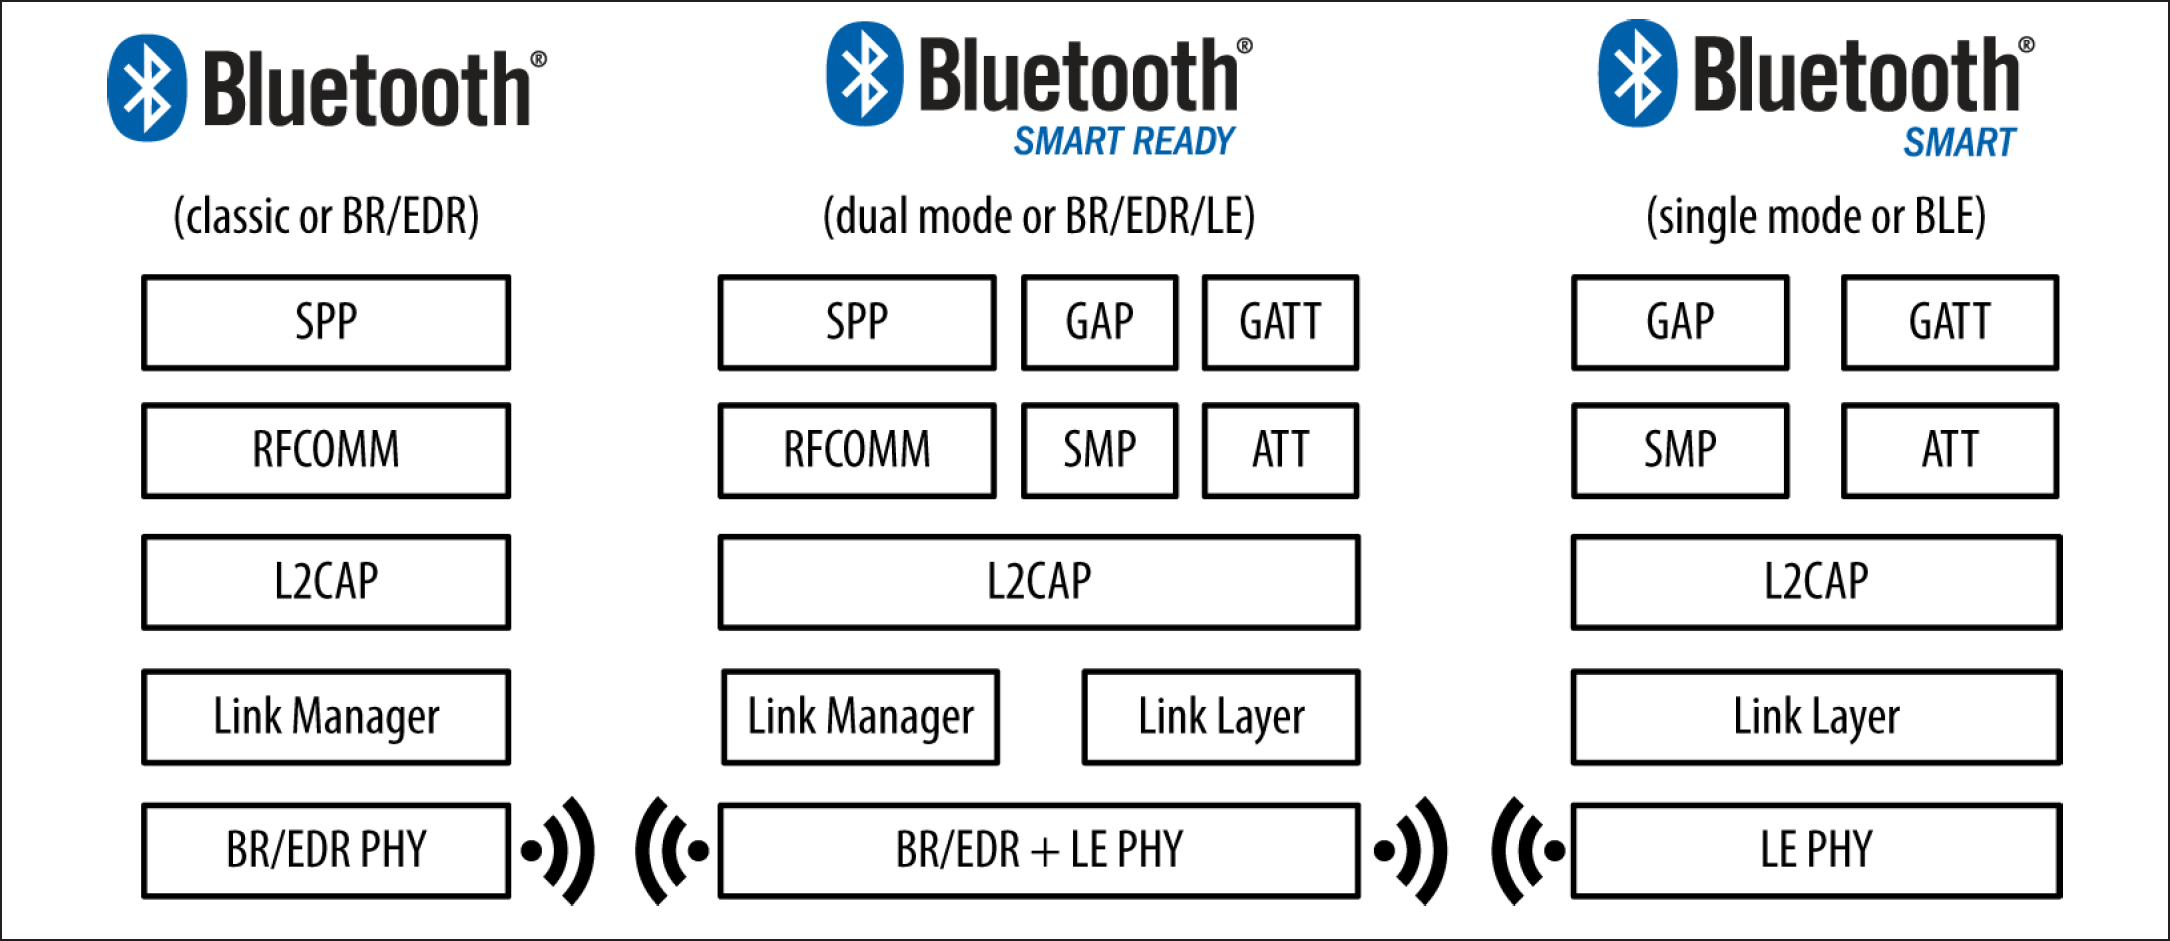
\includegraphics[width = \textwidth]{images/Dual mode bluetooth devices.png}
    \caption{Stack protocollare Bluetooth}
    \label{fig:stack_ble}
\end{figure}

\subsubsection{Aspetti Tecnici}
Lo \textit{spettro di frequenza} in cui opera BLE è compreso tra 2.4000 - 2.4835 GHz, segmentato in 40 canali con un ampiezza di 2 MHz, consentendo un data-rate massimo di 2 Mbps dalla specifica 5.0. \\
Il \textit{raggio di copertura} dipende in modo significativo dall'ambiente circostante e dalla modalità di comunicazione utilizzata; solitamente ha un range di copertura 10 - 30 metri. \\
Anche il \textit{consumo energetico} varia ampiamente, esso è legato all'implementazione, ai diversi parametri BLE e al chipset utilizzato. Generalmente, il consumo di corrente di un chipset BLE durante una trasmissione radio è inferiore a 15 mA. Rispetto al Bluetooth classico, il consumo energetico è ridotto ad un decimo. Nei contesti in cui il duty cycle è piuttosto basso, una batteria tampone potrebbe avere una durata dai 5 ai 10 anni.\\
La \textit{sicurezza} è opzionale per la comunicazione BLE e spetta allo sviluppatore implementarla e la scelta tra i vari livelli di sicurezza supportati. In merito alla crittografia, BLE utilizza AES CCM con una chiave di 128 bit.\\
Le versioni di Bluetooth (riferito a BLE) sono retro compatibili tra loro. Tuttavia, la comunicazione potrebbe essere limitata alle funzionalità della versione precedente.

\subsubsection{Vantaggi e Limitazioni di BLE}
Come tutte le tecnologie, anche BLE presenta dei vantaggi e delle limitazione. Come menzionato precedentemente, BLE è più adatto per applicazione che necessitano di trasmissioni relativamente brevi e che impiegano poche quantità di dati. Tra le limitazioni abbiamo:
\begin{itemize}
    \item \textit{Data Throughput}: una larghezza di banda ridotta (non adatta per applicazione che necessitano trasferimento di dati di grandi dimensioni). La velocità di trasmissione dati è limitata alla velocità fisica della radio Bluetooth, ovvero alla velocità con cui la radio trasmette i dati. Questo tasso dipende anche dalla versione di BLE utilizzata. Per la versioni Bluetooth 4.2 o procedenti il limite è di 1 Mbps mentre, per le versioni superiori il tasso trasmissivo varia (tra 1 Mbps e 2 Mbps) in base alla modalità e al livello PHY utilizzato.
    
    \item \textit{Range di copertura}: BLE è stato progettato per applicazioni a corto raggio, in cui si necessita di una limitata comunicazione. Ci sono diversi \textit{fattori} che limitano il range, tra cui: 
    \begin{itemize}
        \item lo spettro di frequenza ISM 2.4 GHz, fortemente influenzato da ostacoli come oggetti metallici, pareti e acqua (specialmente il corpo umano) ed utilizzato da molte altre tecnologie come wifi, ZigBee, Bluetooth classic, etc.
        \item performance e design dell'antenna adottata dal dispositivo BLE.
        \item orientamento del dispositivo.
    \end{itemize}
    
    \item richiede un \textit{Gateway} per connettere gli end-devices ad Internet.
\end{itemize}

\noindent Nonostante le limitazioni appena menzionate, BLE presenta alcuni vantaggi e benefici significativi rispetto ad altre tecnologie simili, tra cui:
\begin{itemize}
    \item \textit{Consumi energetici ridotti}: BLE ha un consumo energetico ridotto rispetto ai suoi competitors. Lo standard è stato ottimizzato al fine di ridurre i consumi, difatti spegne la radio il più possibile, oltre ad inviare piccole quantità di dati a basse velocità di trasferimento.
    \item \textit{Basso costo} dei moduli e dei chipset BLE
    \item la presenza di questa \textit{tecnologia nella maggior parte degli smartphone presenti sul mercato}. Questo è probabilmente il più grande vantaggio che BLE ha sui suoi concorrenti.
\end{itemize}

\subsection{Architettura}
\subsubsection{Physical Layer (PHY)}
Il livello fisico corrisponde all'hardware usato per consentire la comunicazione per la modulazione e demodulazione dei dati. La radio opera nella banda ISM (Industrial, Scientific, Medical) la quale risulta divisa in 40 canali (Radio Frequenze) separati da 2MHz.\\
Tre di questi canali (37, 38 e 39) sono usati come \textit{Primary Advertising Channel} per impostare le connessioni ed inviare messaggi broadcast, mentre i restanti 37 canali, definiti \textit{Data Channel}, sono usati per trasferire i dati durante una connessione.\\

\noindent I canali Advertising risultano sparsi, come mostrato in figura \ref{fig:frequency_channel}, per evitare interferenze radio tra due dispositivi che pubblicizzano la loro presenza contemporaneamente, nella medesima area, sfruttando due frequenze differenti. Inoltre, la scelta è ricaduta su tali frequenze al fine di limitare le interferenze con i canali Wi-Fi maggiormente usati.

\begin{figure}[!ht]
    \centering
    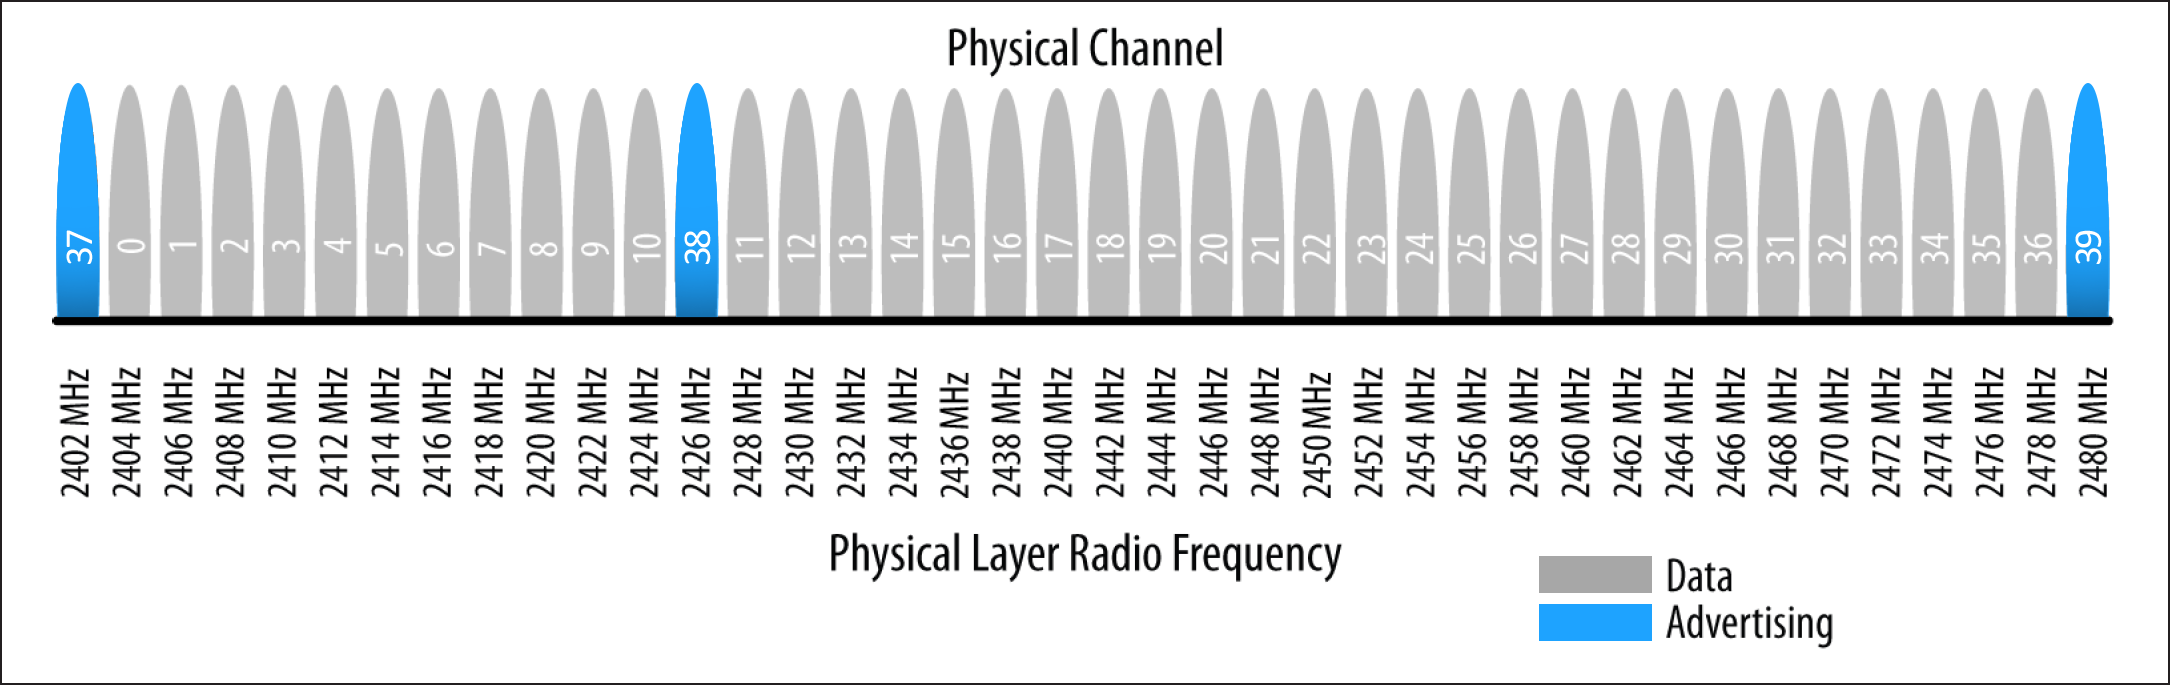
\includegraphics[width = \textwidth]{images/Physical Channel BLE.png}
    \caption{Frequency Channel}
    \label{fig:frequency_channel}
\end{figure}

\noindent Lo standard adotta la tecnica \textit{Frequency Hopping Spread Spectrum} (FHSS), che consente a due dispositivi di cambiare repentinamente frequenza rispettando uno schema apparentemente casuale ma in realtà definito a priori. \\
Il prossimo canale da adottare per un determinato intervallo di tempo viene scelto attraverso la seguente funzione: $ c'=(c+h) \bmod{37}$, in cui $c$ indica il canale attuale, $h$ indica il salto da eseguire e $c'$ denota il prossimo canale per proseguire la comunicazione. L'operazione $\bmod{37}$ consente di muoversi solo nel range dei canali Data. Il valore di $h$, che determina il pattern per la comunicazione, è comunicato dal master nel momento in cui viene stabilita una nuova connessione, all'interno del \textit{connection request packet}.\\
La tecnica FHSS cerca, tra l'altro, di minimizzare gli effetti delle potenziali interferenze radio presenti nell'ambiente circostante (altri dispositivi che usano la banda 2.4 GHz), andando a selezionare uno dei 37 canali disponibili per un determinato intervallo di tempo.\\

% https://www.electronics-notes.com/articles/connectivity/bluetooth/radio-interface-modulation-channels.php
\noindent La tecnica di modulazione usata in BLE per codificare l'informazione digitale in un segnale analogico corrisponde alla Gaussian Frequency Shift Keying (GFSK).
Tale tecnica prevede di rappresentare l'informazione digitale e quindi il bit 1 e bit 0 adoperando due frequenze distinte, rispettivamente una deviazione di frequenza positiva e una negativa rispetto alla portante principale. Il segnale modulato viene successivamente filtrato attraverso una curva Gaussiana per garantire che le bande laterali non eccedono troppo rispetto alla portante principale e per rendere più fluide le transizioni. Così facendo si ottiene un'ampiezza di banda di 1 MHz.\\
%Con le versioni successive, per garantire delle velocità di trasmissione maggiori sono state introdotte delle tecniche di Phase Shift Keying (PSK) che prevedono una modifica nella fase del segnale per differenziare i due valori binari. Nello specifico le due tecniche adottate sotto il nome di Enhanced Data Rate (EDR) a partire da Bluetooth 2 sono la $\pi/4$ DQPSK e 8DPSK. Si passa da una tecnica all'altra in base al rumore presente nel canale, se le condizioni sono ottime si adopera la 8DPSK consentendo di raggiungere velocità di trasmissioni massime di 3 Mbps, altrimenti si adopera la $\pi/4$ DQPSK che consente un massimo di 2 Mbps. La tecnica di trasmissione dati avanzata, EDR, è implementata come funzionalità aggiuntiva in modo che i dispositivi risultano essere compatibili con le versioni precedenti.\\

\noindent Le potenze del trasmettitore Bluetooth sono piuttosto basse, sebbene ci sono quattro diverse classi energetiche (+20, +10, +4 e 0 dBm) che dipendono dall'uso previsto e dalla distanza di copertura richiesta. Il controllo della potenza è consigliabile utilizzarlo per conservare la carica della batteria o ridurre le interferenze con le altre apparecchiature. Il livello di potenza appropriato può essere definito in base al RSSI. La Receiver Sensitivity, ovvero il livello di potenza più basso con la quale è in grado di \textit{rilevare} un segnale RF e \textit{demodulare} i dati contenuti in esso, per i dispositivi che adottano la tecnologia BLE corrisponde a -70 dBm.

\subsubsection{Link Layer (LL)}
% https://medium.com/@pcng/ble-protocol-stack-controller-2d2d5371deec
Il livello di collegamento si interfaccia direttamente con il livello fisico e fornisce un livello di astrazione e il modo per interagire con la radio. Solitamente implementato come una combinazione di hardware e software custom.\\
La parte hardware definisce alcune funzionalità automatizzate, tra cui: Preambolo, Indirizzo d'accesso, individuazione del protocollo adoperato, la generazione e verifica del CRC, la generazione del pattern casuale ($h$) e la cifratura attraverso l'algoritmo AES.
La parte software del Link Layer lo stato dei collegamenti della radio, ovvero il modo in cui il dispositivo si collega ad altri dispositivi. \\
Un dispositivo BLE può agire come master o come slave. Il dispositivo che avvia la connessione sarà il master e i dispositivi che tramite messaggi di Advertsiment comunicano la propria presenza e accettano le connessioni, saranno i slave. 
Solitamente, il ruolo del master è rappresentato da dispositivi con più risorse, come smartphone o tablet, mentre per i dispositivi con vincoli di memoria e a basso costo, come i microcontrollori o i sensori, è riservato il ruolo dello slave.\\

\noindent Il livello di collegamento consente di definire i seguenti ruoli:
\begin{itemize}
    \item \textit{Advertiser}: dispositivo che invia pacchetti Advertising.
    \item \textit{Scanner}: dispositivo che esegue scansioni per individuare la presenza di altri dispositivi nel suo raggio di comunicazione, individuabili tramite la ricezione di pacchetti Advertising.
    \item \textit{Master}: dispositivo che inizializza la connessione. \MakeUppercase{é} responsabile della gestione della connessione, dell'impostazione dei parametri da utilizzare, compresi i timing dei vari eventi, all'interno di una connessione.
    
    \item \textit{Slave}: dispositivo che accetta una richiesta di connessione e si sincronizza con il clock del master.
\end{itemize}

\noindent Quando un dispositivo emette messaggi pubblicitari (Advertiser) attraverso i canali Advertising, consente agli altri device, che sono in una fase di scansione (Scanner), di individuarlo e avere la possibilità di connettersi. Nel momento in cui un Advertiser viene individuato, lo Scanner può decidere di inviare una richiesta di connessione, nella quale è incluso il valore $h$ per definire lo schema di salto di frequenza, per i due dispositivi, durante la connessione. Dopo che l'Advertiser accetta, entrambi passano allo stato \textit{Connection}, assumendo per l'Advertiser il ruolo di Slave e per lo Scanner il ruolo di Master. 
Una \textit{connessione} la possiamo definire semplicemente come una sequenza di scambi di dati tra slave e master in momenti prestabiliti. Lo scambio di informazioni, all'interno di una connessione avviene adoperando i canali Data e tramite pacchetti Data (con 27 byte di payload), i quali consentono il trasporto di informazioni utente in entrambe le direzioni.\\
Nello specifico, gli stati in cui si possono trovare i dispositivi BLE sono i seguenti:

\begin{figure}[!ht]
    \centering
    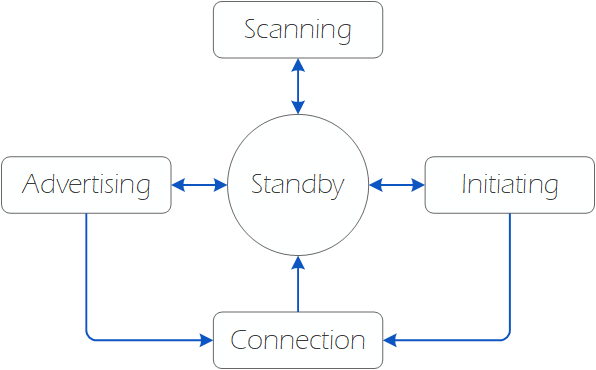
\includegraphics[width = \textwidth]{images/Link layer states.png}
    \caption{Stati Link Layer}
    \label{fig:link_layer_states}
\end{figure}

\begin{itemize}
    \item \textit{Standby}: lo stato in cui il dispositivo non trasmettere e non riceve informazioni. In questo stato è possibile accedere da qualsiasi altro stato.
    
    \item \textit{Advertising}: lo stato in cui il dispositivo invia pacchetti di Advertising individuabili da altri device presenti nell'ambiente circostante. Il dispositivo nello stato di Advertising è conosciuto come Advertiser.
    
    \item \textit{Scanning}: lo stato in cui il dispositivo scansiona l'area circostante in cerca di pacchetti Advertsing inviati dagli Advertiser. Il dispositivo nello stato di Scanning è conosciuto come Scanner.
    
    \item \textit{Initiating}: lo stato assunto dal dispositivo che ha ricevuti dei pacchetti Advertising da uno specifico dispositivo e decide di stabilire una connessione con esso.
    
    \item \textit{Connection}: lo stato in cui il dispositivo ha stabilito una connessione con un altro device e regolarmente si scambiano informazioni.
\end{itemize}

\noindent Dallo stato Standby è possibile accedere a qualsiasi stato ad eccezioni di Connection, accessibile solo dallo stato Initianing e Advertising.

\paragraph{Device Address}
I dispositivi Bluetooth sono identificabili attraverso un indirizzo di 48 bit (6 byte), \textit{Bluetooth Device Address}, che può essere un \textit{Public device address} o un \textit{Random device address}. 
L'indirizzo \textit{Public} è assegnato al dispositivo al momento della fabbricazione e non cambierà mai per tutta la vita del dispositivo, ed è registrato presso l'autorità IEEE così come avviene per l'indirizzo MAC per i device Wi-Fi o Ethernet. 
L'indirizzo \textit{Random} può essere programmato sul dispositivo o generato dinamicamente in fase di esecuzione. Quest'ultimo è più popolare poiché non richiede la registrazione presso l'ente IEEE.\\
Per quanto riguarda l'indirizzo Random possiamo avere due sottotipi: Static e Private Address.

\begin{itemize}
    \item \textit{Static Address}: in genere sono utilizzati come sostituti degli indirizzi Public. Esso è semplicemente un indirizzo casuale che può essere generato ogni volta che il dispositivo si avvia o definito a priori in modo che rimane invariato ad ogni accensione. Non può essere modificato finché il dispositivo è in esecuzione.
    \item \textit{Private Address}: generati a partire da una Identity Resolving Key (IRK) e da un numero casuale di 24 bit. A differenza dei precedenti, possono essere cambiati spesso, anche mentre il dispositivo è in funzione. Il loro utilizzo è legato alle questioni di privacy, ad esempio si può cambiare l'indirizzo per evitare che il dispositivo venga identificato e rintracciato da un device sconosciuto. Il processo di identificazione può avvenire solo se in possesso della IRK distribuita dal device durante la fase 3 mostrata nel grafico \ref{fig:phasis_pairing_bonding}.
\end{itemize}

\paragraph{Advertising e Scanning}
BLE ha solo un formato per i pacchetti e possiede due tipi di pacchetti (Advertising e Data). 
I pacchetti Advertising possono avere un payload di dimensioni fino ad un massimo 31 bytes. Essi sono inviati in broadcast dal dispositivo Advertiser senza essere a conoscenza della presenza di un eventuale device Scanner. L'invio avviene con un intervallo prefissato compreso tra 20ms e 10.24ms, con incrementi di 625 $\mu s$. Più corto è l'intervallo e più alta è la frequenza con cui i pacchetti sono inviati in broadcast, aumentando così la probabilità di essere intercettati dai dispositivi in ascolto ma compromettendo la durata della batteria, difatti l'uso di una frequenza più alta comporta un maggior consumo di energia. Solitamente si tende a privilegiare un intervallo alquanto lungo che fornisce equilibrio tra connettività rapida e consumo energetico ridotto.\\
Il processo di Advertising predispone al massimo tre canali e poiché l'advertiser e lo scanner non risultano sincronizzati, un pacchetto Advertising verrà ricevuto sono quando i rispettivi intervalli di invio e ascolto si sovrapporranno. I parametri che consentono di gestire tale situazione sono: \textit{Scan Type} che può essere passivo o attivo, \textit{Scan Window} indica per quanto tempo essere in ascolto sui canali di Advertising e \textit{Scan Interval} indica quanto spesso eseguire il processo di ascolto. Difatti lo Scanner sarà in ascolto sui tre canali di Advertising per l'intera durata della Scan window ed ogni Scan Interval.\\ 
% Immagine Passive e active scanning pagina 35
In merito alla scansione dei pacchetti Advertising sono definite due modalità: \textit{Passive scanning} e \textit{Active scanning}.
Durante una procedura passiva, lo scanner semplicemente si mette in ascolto di eventuali messaggi, e l'Advertiser non sarà mai a conoscenza se uno o più pacchetti saranno effettivamente ricevuti dai dispositivi circostanti.
Con la procedura attiva, lo scanner inoltra una Scan Request dopo aver ricevuto un pacchetto Advertising. In tal modo, l'Advertiser riceverà la richiesta e sarà per prima cosa a conoscenza dell'avvenuta ricezione e dopodiché procederà a rispondere attraverso una Scan Response. L'uso di Scan Request e Response consente all'Advertiser di inviare informazioni aggiuntive che non rientrerebbero nel normale pacchetto Advertising. \\
I pacchetti pubblicitari sono utilizzati dai livelli superiori, più specificamente, dal GAP per differenziare le modalità operative e definire le procedure.

\paragraph{Connections}
Per stabilire una connessione tra due dispositivi Bluetooth, per prima cosa si deve avere un dispositivo con il ruolo di Advertiser ed uno con il ruolo di Scanner. Detto ciò, il dispositivo nello stato di Advertising inizia ad inviare pacchetti per testimoniare la sua presenza e il dispositivo nello stato di Scanning , nel mentre, deve scansionare l'intera area al fine di acquisire i pacchetti inviati dall'altro device. I pacchetti riscontrati, verranno filtrati attraverso il Bletooth Address o in base alla tipologia. \\
Quando, a seguito dell'analisi dei pacchetti intercettati, viene riscontrata la presenza di un potenziale slave, il nodo Central procederà con l'invio di una richiesta di connessione (Connection Request packet). Il nodo periferico, è sempre in ascolto per un breve intervallo di tempo sugli stessi canali utilizzati per inviare pacchetti Advertising. Ciò gli consente di ricevere il pacchetto Connection Request il quale innescherà un processo di connessione tra i due dispositivi, il che comporterà l'invio di una risposta da parte dello slave, sempre se desidera procedere in tale direzione.\\
Solo nel momento in cui verrà ricevuto quest'ultimo pacchetto la connessione si può considerare stabilita, altrimenti essa risulta solo creata. Solo dopo aver instaurato la connessione è possibile definire il nodo Central come Master e il nodo Peripheral come Slave.\\

\begin{figure}[!ht]
    \centering
    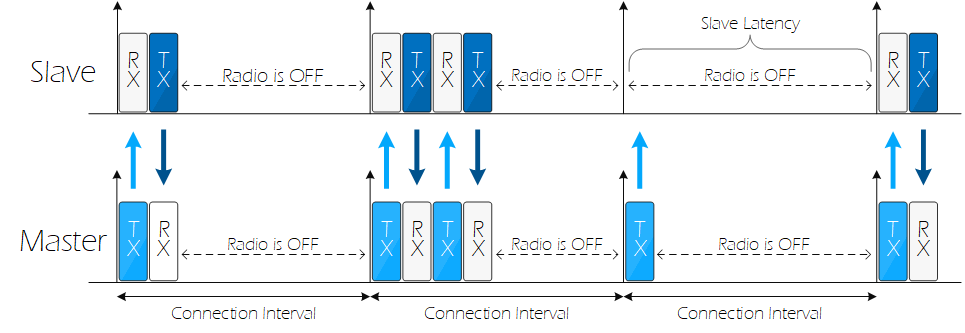
\includegraphics[width = \textwidth]{images/Connection events.png}
    \caption{Connection events}
    \label{fig:connection_events}
\end{figure}

\noindent La connessione è semplicemente una sequenza di scambio di dati tra master e slave, in modo alternato e in istanti prestabiliti. L'invio alternato dei pacchetti dati costituisce il \textit{Connection Event}. Tale evento prevede sempre la presenza di almeno un pacchetto inviato dal master a cui fa seguito la risposta da parte dello slave. Se il master non riceverà risposta da parte dello slave chiuderà il connection event e riprenderà l'invio al successivo connection event. Il tempo trascorso tra l'inizio di due connection event successivi è chiamato \textit{Connection Interval}. Tale tempo corrisponde ad un valore compreso tra 7.5 ms (alto throughput) e 4 s (basso throughput) con soglie di 1.25 ms. Altri parametri impostati prima di stabile la connessione riguardano lo \textit{Slave Latency} e \textit{Connection Supervision Timeout}.\\
Il parametro slave latency consente al dispositivo peripheral di scegliere un numero consecutivo di connection event da saltare senza compromettere la connessione. Questo consente al dispositivo di restare spento per un lungo periodo di tempo, potenzialmente riducendo i consumi energetici.\\
Il parametro connection supervision timeout definisce il tempo massimo tra la ricezione di due pacchetti dati prima che la connessione venga considerata persa. L'intervallo è compreso tra 100 ms e 32 s con soglie di 10 ms.\\

\noindent Un nodo BLE prima di accedere al contenuto di un pacchetto ricevuto, può attuare un meccanismo di filtering il quale consente di scartare quei pacchetti a cui non è interessato. Una \textit{White List} è semplicemente un lista di Bluetooth device address popolata dall'host e memorizzata ed utilizzata dal controller. Tale lista può essere utilizzata per i stati di Advertising, Scanning e Initiating.


\subsubsection{Host Controller Interface (HCI)}
Come introdotto in precedenza, la specifica Bluetooth definisce l'HCI come uno standard per consentire l'interazione tra Host e Controller all'interno di uno stack BLE. Questi livelli possono essere implementati come chipset differenti o possono coesistere nel medesimo chipset. Nel caso in cui i due livelli sono in due chipset differenti, il livello HCI sarà implementato su un'interfaccia di comunicazione fisica.ì, mentre nel caso in cui si trovano nel medesimo chipset, allora HCI sarà un'interfaccia logica.\\
Il ruolo di HCI layer prevede la trasmissione dei comandi dal host verso il controller e viceversa.

\subsubsection{Logical Link Control and Adaptation Protocol (L2CAP)}
Il livello L2CAP fornisce due funzionalità importanti per lo standard BLE. Innanzitutto, consente di incapsulare tutti i protocolli degli strati superiori all'interno di un pacchetto standard BLE. Inoltre, esegue il processo di frammentazione nel momento in cui, dai livelli superiori, giunge un pacchetto le cui dimensioni risultano maggiori dello standard BLE (Payload LL layer 27 byte e 4 byte header L2CAP); mentre, nel caso in cui giunge un pacchetto frammentato, attende la ricezione di tutti i frammenti prima di procedere con la creazione del pacchetto originale ed l'invio all'entità appropriata di livello superiore. La frammentazione è poco adoperata in primo luogo perché richiede un dispendio piuttosto elevato di energia e in più perché gli standard utilizzati ai livelli superiori consentono di fornire unità dati che si adattano alla dimensione massima del payload L2CAP, di 23 byte in BLE. \\
Per BLE, il protocollo L2CAP è responsabile di due protocolli principali: Attribute Protocol (ATT) e Security Manager Protocol (SMP). Il protocollo ATT costituisce la base per lo scambio di informazioni per applicazioni BLE, mentre SMP fornisce un framework per generare e distribuire le chiavi di sicurezza tra i nodi.

\subsubsection{Attribute Protocol (ATT)}
L'Attribute Protocol è un protocollo che definisce la comunicazione tra due dispositivi con il ruolo di client e server per accedere agli \textit{attributi} forniti dal server. Più specificamente, definisce come un server espone i propri dati ad un client e come tali dati risultano strutturati.
Il server è quel dispositivo che accetta richieste eseguite da un dispositivo ed invia risposte, notifiche e indicazioni in merito ai propri attributi. % Esempio di Server: Termometro quando espone la temperatura dell'ambiente circostante
Il client, invece è quel dispositivo che interagisce con il server con lo scopo di entrare a conoscenza dei dati esposti dal server e all'occorrenza controllare il comportamento del server. Il client non è a conoscenza degli attributi forniti dal server, quindi prima deve informarsi sulla presenza e sulla natura di tali attributi attraverso la procedura di service discovery, dopodiché può dare il via alle operazioni di reading e writing degli attributi individuati.\\
I dati messi a disposizione dal server sono organizzati secondo una struttura dati predefinita e generica che prende il nome di \textit{attributo}, manipolati e acceduti attraverso il protocollo GATT.\\
A ciascuno attributo è assegnato un identificativo univoco di 128 bit (16 byte),\textit{Universally Unique Identifier} o UUID, che ne specifica il tipo e la natura dei dati, oltre a consentire l'accesso alla risorsa. Per questioni di efficienza, la specifica BLE definisce un formato addizionale di 16 bit. Il formato ridotto (16 bit) può essere adottato solo per quegli attributi definiti nella specifica Bluetooth (definiti come standard da parte di Bluetooth SIG). \\
Nel caso in cui si ha la necessità di una specifica non definita dallo standard SIG, è possibile implementarla e assegnargli un UUID specifico di 128 bit, denominata come \textit{vendor-specific UUID}.
%% Attribute handle
L'\textit{attribute handle} è un identificatore di 16 bit, presente in ogni attributo, che permette ad una specifica risorsa di essere reperibile dal client, e garantisce l'identificazione univoca per tutta la durata di una connessione.\\
%% Type e Value
Il campo \textit{type} incluso all'interno di un attributo è legato al rispettivo UUID e determina il tipo di dato presente nel campo \textit{value} e i meccanismi individuabili nella fase di discovery per poter accedere a tale attributo.\\
%% Permission
I \textit{permessi} sono meta-dati presenti in ogni attributo e specificano quale operazione ATT può essere eseguita e quali sono i requisiti di sicurezza per potervi accedere. Possono essere distinti in: Access Permission, Encryption e Authorization.
\begin{itemize}
    \item \textit{Access Permission}: determina se il client ha il permesso in lettura o in scrittura (o entrambe) al valore di un attributo.\\
    \textit{None} indica che il client non ha i permessi né per la lettura né per la scrittura.
    \textit{Readable} indica che l'attributo può essere accessibile solo in lettura.
    \textit{Writable} indica che il client ha il permesso in scrittura per l'attributo.
    Se l'attributo presenta entrambi i permessi, \textit{Readable} e \textit{Writable}, allora il client può accedere sia in lettura che in scrittura.
    
    \item \textit{Encryption}: determina il livello di sicurezza richiesto per far sì che il client possa accedere ad un determinato attributo.
    \textit{No encryption required} indica che l'attributo è accessibile senza nessun livello di sicurezza, le informazioni sono accessibile senza avere una comunicazione cifrata.
    \textit{Unauthenticated encryption required} prevede l'utilizzo di una connessione cifrate per accedere all'attributo, ma non necessita che le chiavi di cifratura siano autenticate.
    \textit{Authenticated encryption required} garantisce il livello di sicurezza più alto, vale a dire che per accedere all'attributo la connessione deve essere crittografata con una chiave autenticata.
    
    \item \textit{Authorization}: determina se l'accesso all'attributo prevede l'autorizzazione da parte dell'utente. Le alternative in questa circostanza sono \textit{No authorization required} e \textit{Authorization required}.
\end{itemize}
\noindent Il \textit{permesso}, in realtà, non viene definito o individuato attraverso il protocollo ATT, ma bensì attraverso il protocollo GATT o il livello Applicativo.\\

\noindent Il protocollo ATT opera in termini di attributi e tramite essi è in grado di fornire una serie di Protocol Data Unit (PDU o packet) che consentono ad un client ad accedere agli attributi su un server.

\subsubsection{Security Manager (SM)}
La sicurezza è una delle maggiori preoccupazione espresse nel contesto dei sistemi IoT. Tra le problematiche più comuni in merito alla sicurezza per sviluppatori e produttori di dispositivi, si hanno:
\begin{itemize}
    \item \textit{Autenticazione}: essere sicuro che l'altra parte sia davvero chi afferma di essere.
    \item \textit{Integrità}: assicura che i dati non risultano corrotti e manomessi da un utente o dispositivo non autorizzato a trattarli.
    \item \textit{Riservatezza}: essere sicuri che i dati non siano leggibili da dispositivi o utenti non autorizzati.
    \item \textit{Privacy}: indica quanto è privata una comunicazione e se una terza parte è in grado di tracciare il nostro dispositivo, soprattutto dal suo identificativo.
\end{itemize}
In merito alla sicurezza ed ai concetti appena espressi, purtroppo ci sono differenti tipi di attacchi realizzatati da un soggetto malintenzionato. Alcuni di essi riguardano:
\begin{itemize}
    \item \textit{Intercettazione Passiva}: si verifica nel momento in cui un malintenzionato si posiziona tra i due dispositivi, ascoltando la comunicazione e riuscendo a comprendere il suo contenuto. Solitamente ottenendo l'accesso alla chiave di cifratura nel momento in cui i dati risultano cifrati.
    \item \textit{Intercettazione Attiva}: attacco conosciuto anche con il nome di \textit{Man-In-The-Middle} (MITM). In questa circostanza il soggetto malizioso finge di essere entrambi i dispositivi all'interno di una comunicazione. Può intercettare la comunicazione e indirizzarla nuovamente ed eventualmente inserendo anche dati aggiuntivi all'interno dei pacchetti, il tutto avviene in modo tale che le due entità non si rendano conto che l'attacco sta accadendo.
    \item \textit{Monitoraggio della Privacy e dell'identità}: in questa tipologia di attacco, il dispositivo è tracciato tramite l'indirizzo Bluetooth con la possibilità di individuare la sua posizione e correlandola con il suo comportamento.
\end{itemize}

\noindent Security Manager è sia un protocollo che una serie di algoritmi di sicurezza progettati per fornire la capacità di generare e scambiare chiavi di sicurezza al fine di garantire una comunicazione attraverso un collegamento criptato. Comprende cinque funzioni:
\begin{itemize}
    \item \textit{Pairing}: procedura mediante la quale viene generata una chiave segreta, condivisa tra i due dispositivi, al fine di costituire un collegamento crittografato e sicuro. Tale chiave risulta essere temporanea, quindi non potrà essere riutilizzata per le connessioni successive.
    
    \item \textit{Bonding}: il processo di creazione e archiviazione della chiave segreta eseguito da entrambi i dispositivi, che consentirà loro di impostare rapidamente un collegamento sicuro anche per le connessioni successive.
    
    \item \textit{Autenticazione}: il processo che consente di verificare che entrambi i dispositivi condividono la stessa chiave segreta.
    
    \item \textit{Crittografia}: il processo prevede di crittografare i dati scambiati tra due dispositivi. In BLE tale processo avviene utilizzando lo standard di cifratura AES a 128 bit, algoritmo di cifratura a chiave simmetrica (significa che la stessa chiave è usata sia per cifrare che per decifrate i dati su entrambi i lati).
    
    \item \textit{Integrità dei messaggi}: il processo che consente di controfirmare i dati e verificare la validità della firma sull'altro dispositivo.
\end{itemize}
Il \textit{Pairing} consente di creare un collegamento sicuro che durerà solo per la durata della connessione, mentre il \textit{Bonding} crea effettivamente un'associazione permanente sotto forma di chiavi di sicurezza condivise utilizzabili per le connessioni future, finché i due nodi non decidono di eliminarle. La fase di boring consente ai due dispositivi, nel momento in cui dovranno creare nuovamente un canale di comunicazione sicuro, di evitare la fase di Pairing.\\

\noindent In BLE i diversi problemi menzionati all'inizio del capitolo sono affrontati per tramite le funzioni appena descritte, ovvero: la \textit{riservatezza} viene garantita attraverso il processo di crittografia dei dati; l'\textit{autenticazione} tramite le funzioni di pairing e bonding; la \textit{privacy} è garantita adottando gli indirizzi privati; e l'\textit{integrità dei dati} viene assicurata tramite il meccanismo di firma digitale.

\begin{figure}[!ht]
    \centering
    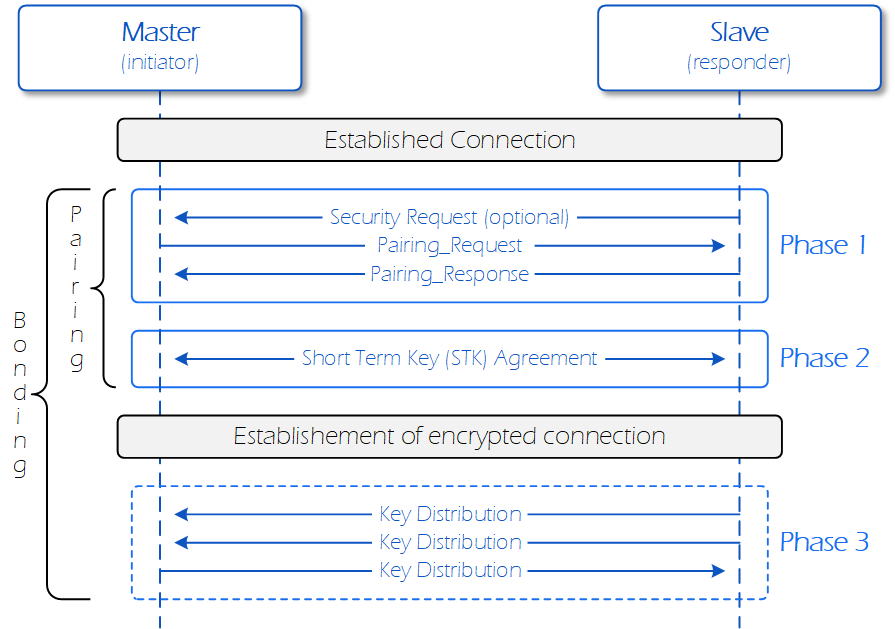
\includegraphics[width = \textwidth]{images/Pairing and Bonding.png}
    \caption{Fasi del processo di sicurezza in BLE}
    \label{fig:phasis_pairing_bonding}
\end{figure}

\noindent Il processo che consente di rendere il collegamento tra due dispositivi sicuro (mostrato in figura \ref{fig:phasis_pairing_bonding}), prevede innanzitutto uno scambio di informazioni per generare una chiave di sicurezza temporanea (fase 1) e, opzionalmente tale fase può essere avviata da una richiesta eseguita da parte dello slave per l'avvio di una procedura di sicurezza. Lo scambio di informazioni avviene attraverso lo scambio di messaggi tra master e slave, ed è il master ad avviare il processo inviando il messaggio \textit{Pairing Request} a cui lo slave risponde con il messaggio \textit{Pairing Response}, a tal proposito il master è denominato \textit{initiator} mentre lo slave \textit{responder}. Le informazioni scambiate in questa fase determinano il metodo da utilizzare per la procedura di Pairing, ovvero la fase 2.\\
Dopo di che, (fase 2) entrambi i dispositivi generano in modo indipendente una chiave cifrata temporanea (\textit{Short Term Key} o STK) e la usano per crittografare la connessione. 
Una volta che la connessione risulta essere cifrata e solo se si utilizza la procedura di \textit{Bonding} (fase 3), le chiavi permanenti possono essere distribuite per la memorizzazione e il riutilizzo in un secondo momento. 

\subsubsection{Generic Attribute Profile (GATT)}
Generic Attribute Profile è implementato al di sopra di Attribute Protocol (ATT), aggiunge una gerarchia e una modello di astrazione ai dati. Adoperato solo dopo avere instaurato una connessione tra due dispositivi, risulta l'elemento cardine all'interno di una comunicazione BLE. Il protocollo GATT definisce la struttura e le regole attraverso cui i dati, esposti dal server, devono essere scambiati tra due applicazioni. A tal proposito sono introdotti concetti come \textit{Services} e \textit{Characteristics} per specificare la struttura dei dati e le procedure per interfacciarsi con gli attributi definiti (come service discovery, la lettura e  la scrittura delle caratteristiche, le notifiche, etc).\\
Il ruolo di client e server non è definito a priori, esso è determinato in base alla circostanza ($request \leftrightarrow{response}$, $indication \leftrightarrow{confirmation}$ e $notification$). Vale a dire che un dispositivo, all'interno di una connessione, può agire sia come server mettendo a disposizione i propri dati per i client, sia come client leggendo dati messi a disposizione da altri server.

\paragraph{Profiles, Services e Characteristics}
Il protocollo GATT prevede di raggruppare gli attributi correlati tra loro, al fine di definire una funzionalità specifica del server, attraverso una struttura dati gerarchica denominata \textit{service}.

\begin{figure}[!ht]
    \centering
    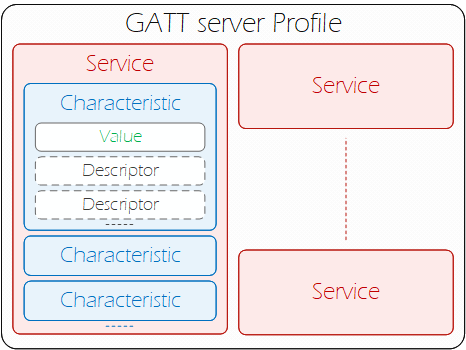
\includegraphics[width =\textwidth]{images/Services GATT.png}
    \caption{Profile, Services e Characteristics}
    \label{fig:profile_GATT}
\end{figure}

\noindent Un service è costituito sempre da una \textit{service declaration}, posta sempre come primo attributo, e seguita da zero o più \textit{characteristics}. A seguito della dichiarazione possono essere aggiunti zero o più attributi \textit{include definitions}, i quali consentono di richiamare altri service al fine di estendere le funzionalità. Tale campo contiene tutti i dettagli richiesti affinché il client possa far riferimento al service aggiunto.\\
I service possono essere divisi in primario e secondario. Il primary rappresenta le funzionalità standard fornite dal server GATT, mentre il secondary definisce delle funzionalità aggiuntive e può essere incluso solo al seguito di un primary.\\

\noindent La caratteristica, sempre compresa in un service, rappresenta l'informazione che il server vuole esporre ai client. Comprende sempre almeno due attributi: \textit{characteristic declaration} che fornisce informazioni in merito ai dati che detiene e \textit{characteristic value} contenente i dati effettivi sui quali il client può accedere sia in lettura che in scrittura. Quest'ultimo campo può essere seguito da zero o più \textit{descriptors} in grado di espandere ulteriormente i meta-dati contenuti nella dichiarazione.\\
L'attributo \textit{declaration}, ha l'autorizzazione ad essere acceduto solo in lettura ed è ripartito in diversi campi, tra cui il campo \textit{Properties} contenente le operazioni e le procedure eseguibili dal client sulla specifica caratteristica.\\
% Ad esempio, il \textit{battery service} definito da SIG contiene una caratteristica chiamata \textit{battery level}. 

\noindent \textit{Profiles} sono molto più ampi nella definizione rispetto ai service e il loro compito è di definire il comportamento, sia del client sia del server, quando si tratta di servizi, caratteristiche e persino connessioni e requisiti di sicurezza. I service e le rispettive specifiche invece, si occupano dell'implementazione solo lato server. Così come per i service, anche per i profile ci sono standard definiti da Bluetooth SIG e generalmente comprendono la definizione dei ruoli e relazioni tra server e client, i requisiti per i service e come utilizzare i service e le carattertisic richiesti, considerazioni in ambito di sicurezza e dettagli in merito ai requisiti per stabilire la connessione, inclusi Advertising e parametri di connessione.

\subsubsection{Generic Access Profile (GAP)}
Il protocollo Generic Access Profile definisce i ruoli, i modi e le procedure al fine di assicurare l'interoperabilità e lo scambio di informazioni tra dispositivi realizzati da fornitori diversi, oltre a definire un insieme di regole e concetti per regolare e standardizzare le operazione svolte nei livelli sottostanti.
Nello specifico determina come i dispositivi devono eseguire le procedure di controllo come la discovery dei dispositivi e dei services, la gestione dell'instaurazione della connessione, l'instaurazione in un collegamento sicuro, ed eseguire molte altre operazioni fondamentali dello standard BLE.\\

\noindent Tale protocollo definisce i seguenti aspetti legati all'interazione tra dispositivi.
\paragraph{Ruoli}
Ogni dispositivo può operare in uno o più ruoli contemporaneamente e ognuno di essi impone restrizioni e determinati requisiti in merito al comportamento. Alcune combinazioni consentono ai dispositivi di comunicare tra loro e il protocollo GAP stabilisce le interazioni tra tali ruoli. I quali possono essere:
\begin{itemize}
    \item \textit{Broadcaster}: invia periodicamente pacchetti Advertising contenenti i dati. Ottimizzato per applicazioni che necessitano solo distribuire i dati regolarmente. Un ottimo esempio potrebbe essere un termometro in grado di trasmettere le letture a tutti i dispositivi interessati. Il Broadcaster invia dati all'interno di pacchetti Advertising e non attraverso pacchetti Data, utilizzabili solo a seguito di una connessione. In tal modo, i dati sono accessibili a qualsiasi dispositivo in ascolto. Broadcaster si basa sul ruolo Advertiser del Link Layer.
    
    \item \textit{Observer}: nodo improntato sull'ascolto dei messaggi Advertising inviati dai nodi circostanti. Ottimizzato per le applicazioni che desiderano solo raccogliere informazioni provenienti dai nodi Broadcaster. Un esempio potrebbe essere un dispositivo dotato di display tramite il quale mostra i dati delle temperature ricevute da sensori di temperatura broadcaster.  Non ha la capacità di avviare una connessione con l'Advertiser e si basa sul ruolo di Scanner del Link Layer.
    
    \item \textit{Central}: un dispositivo in grado di stabilire connessioni multiple con i nodi e corrisponde al ruolo di Master per il Link Layer. Il protocollo BLE è \textit{asimmetrico}, il che significa che i requisiti del master sono maggiori rispetto a quelli dello slave e, a tal proposito il ruolo di Central è svolto solitamente da dispositivi in possesso di CPU performanti e con ottime capacità di memoria, come lo sono gli smartphone o tablet. Proprio la presenze di tali requisiti rende possibile mantenere connessioni tra più dispositivi. 
    
    \item \textit{Peripheral}: dispositivo che si preoccupa di inviare pacchetti Advertising per consentire ai nodi Central di individuarlo, e successivamente, stabilire una connessione con esso. Una volta che viene instaurata una connessione con un dispositivo Central, diventa noto anche come Slave in tale connessione, arresta l'invio di pacchetti Advertising. Ottimizzato al fine di minimizzare le risorse necessarie per la sua implementazione, in termini di potenza di elaborazione e memoria.
\end{itemize}

\noindent Un'osservazione in merito ai ruoli appena descritti e i ruoli di client menzionati a proposito del protocollo GATT. I ruoli client e server dipendono esclusivamente dalla direzione in cui fluiscono le transazioni di richiesta e risposta in merito ai dati, mentre i ruoli definiti dal protocollo GAP, sopra descritti, rimangono invariati.\\

\noindent Un tipico esempio di applicazioni basate sul ruolo di Broadcaster sono le tecnologie \textit{Beacon}. I Beacon sono dispositivi aventi il solo scopo di pubblicizzare la propria esistenza e trasmettere dati specifici, mentre non sono in grado di accettare connessioni da altri dispositivi.\\

\noindent Il modo in cui un Boardcaster si differenzia da un nodo Peripheral è attraverso i pacchetti Advertising trasmessi dal dispositivo. Esistono due tipi di pacchetti Advertising: alcuni consentono di accettare le connessioni, mentre altri servono solo per pubblicizzare la propria presenza. Quando un dispositivo Central riceve un pacchetto Advertising è in grado di comprendere il ruolo del dispositivo mittente e quindi se è possibile instaurare una connessione.\\
Il principale vantaggio di restare nello stato di Advertisng è che molti dispositivi possono scoprire Advertising Data senza la necessità di instaurare una connessione. Tuttavia, l'aspetto negativo riguarda la mancanza di sicurezza e l'impossibilità di instaurare una comunicazione bidirezionale (dal Central al Broadcaster).

\begin{figure}[!ht]
    \begin{subfigure}{0.5\textwidth}
        \centering
        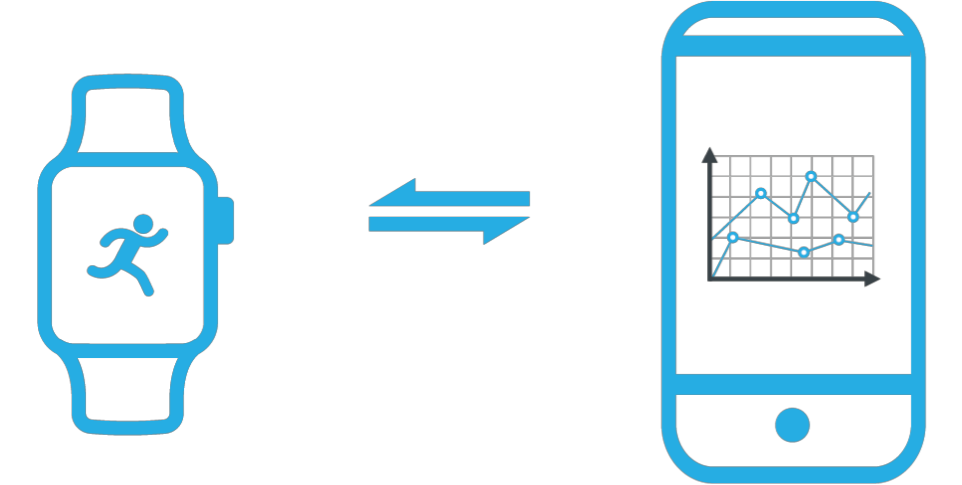
\includegraphics[width=0.85\linewidth]{images/Peripheral - Master.png} 
        \caption{Peripheral - Central}
        \label{fig:subim1}
    \end{subfigure}
    \begin{subfigure}{0.5\textwidth}
        \centering
        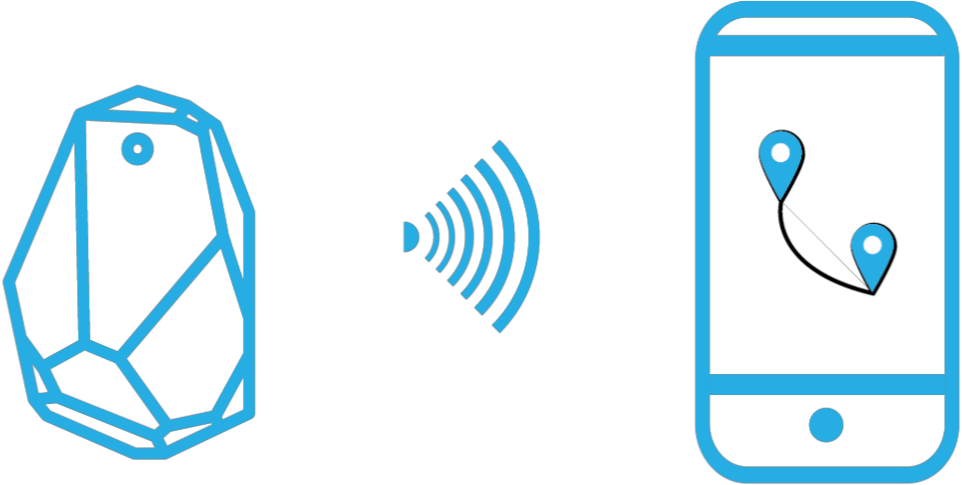
\includegraphics[width=0.85\linewidth]{images/Broadcaster - Observer.png}
        \caption{Broadcaster - Observer}
        \label{fig:subim2}
    \end{subfigure}
    \caption{Ruoli dei dispositivi BLE definiti dal protocollo GAP}
    \label{fig:GAP_roles}
\end{figure}

\noindent Ricapitolando, si può affermare che i ruoli di Broadcaster e Observer necessitano di risorse piuttosto limitate e non garantiscono una comunicazione bidirezionale, poiché rispettivamente provvedono a trasmettere e ricevere informazioni tramite pacchetti Advertising. Gli altri due ruoli, Peripheral e Central, invece necessitano dell'intero stack BLE il che consente loro di supportare una comunicazione bidirezionale. Gran parte delle responsabilità di elaborazione devono essere svolte dal dispositivo centrale consentendo così di ridurre i consumi energetici per i dispositivi periferici e dando loro la possibilità di essere rappresentati attraverso dispositivi sempre più piccoli, con risorse limitate e alimentati a batteria.

\paragraph{Modalità e Procedure}
La modalità è uno stato in cui il dispositivo può passare per un certo periodo di tempo al fine di raggiungere un determinato obiettivo o, più specificamente, consentire ad un nodo ad eseguire una determinata procedura. 
Una procedura è una sequenza di azioni che consentono ad un dispositivo il raggiungimento un determinato obiettivo. Una procedura è solitamente associata ad una modalità su un altro nodo, a tal proposito sono spesso messe in relazione.
Il passaggio da una modalità all'altra può avvenire a seguito di azioni innescate tramite l'interfaccia utente o automaticamente quando richiesto.\\

\noindent La modalità \textit{broadcast} e la procedura \textit{observation} definite da GAP rappresentano l'approccio attraverso il quale i dispositivi possono inviare i dati unidirezionalmente. Un broadcaster invia in broadcast dati senza alcuna conferma o riscontro e non ha nessun modo per verificare se i dati inviati raggiungono effettivamente altri dispositivi, mentre un observer ascolta potenziali broadcaster senza alcuna garanzia di ricevere effettivamente informazioni.\\

\noindent La \textit{discoverability} si riferisce al modo in cui un dispositivo pubblicizza la propria presenza e cosa possono o dovrebbero fare i dispositivi in ascolto con le informazioni ricevute dai dispositivi nelle vicinanze. Ciò non implica necessariamente
l'intenzione di creare una connessione o scambiare i dati. Ci sono diverse modalità in merito alla discoverability che consentono una certa flessibilità ai progettisti di nodi periferici, a seconda della priorità di progettazione come ad esempio durata della batteria piuttosto che tempi di connessione rapidi.\\

\noindent La modalità \textit{connectable} consente di far stabilire una connessione tra un dispositivo central ed uno periferico. A seconda della modalità di creazione di una connessione si riflette sull'uso dei diversi pacchetti Advertising per un dispositivo periferico.

\paragraph{Sicurezza}
Il protocollo GAP in merito alla sicurezza definisce modalità e procedure di sicurezza che specificano il modo in cui i nodi impostano il livello di sicurezza richiesto da un particolare scambio di informazioni e successivamente come viene applicato tale livello di sicurezza. Le funzionalità definite non sono associate ad una particolare modalità o procedura, proprio per questo motivo possono essere utilizzate per aumentare il livello di sicurezza dei dati gestiti da qualsiasi tipo di applicazione.\\

\noindent Gli aspetti di sicurezza per BLE sono basati su due pilastri: il protocollo SM e gli aspetti GAP in merito alla sicurezza.\\
Il protocollo SM implementa gli algoritmi di crittografia e si occupa di tutte quelle funzionalità che consentono lo scambio di dati in modo sicuro tra due dispositivi.\\
GAP definisce una serie di modalità e procedure relative alla sicurezza le quali consentono di instaurare una connessione fidata e in grado di trasportare dati sensibili. Inoltre, GAP espande e specifica ulteriormente l'utilizzo degli strumenti definiti dal protocollo Security Manager al fine di garantire interoperabilità tra dispositivi differenti.

\section{ZigBee}
%%% LIBRO ZIGBEE [1,4,5 ]
ZigBee è uno degli standard molto popolari sul mercato, per reti di sensori a basso costo, a bassa velocità trasmissiva, a basso consumo energetico a a corto raggio \cite{farahani2011zigbee}. ZigBee è definito come protocollo di comunicazione di alto livello, basato sullo standard IEEE 802.15.4, il quale è stato definito per l'implementazione e la standardizzazione di reti Wireless PAN (Personal Area Network) a bassa velocità di comunicazione.\\

\noindent Le applicazioni che prediligono l'uso della tecnologia ZigBee sono alimentate a batteria, e devono soddisfare le caratteristiche definite dalla tecnologia in uso, come: basso costo, bassa potenza, limitata velocità di trasmissione dati, e lunga durata della batteria. Tali applicazioni prediligono un uso molto limitato della radio, difatti il dispositivo spende la maggior parte del suo tempo in modalità risparmio energetico, noto anche come \textit{sleep mode}.
Queste caratteristiche, insieme al funzionamento su uno spettro di frequenze libero, senza licenza, ed essendo un protocollo standardizzato, basato sullo standard IEEE 802.15.4 facilitano lo sviluppo e l'implementazione della rete e la rendono una delle tecnologie wireless più adatte per le applicazioni di smart grid \cite{yi2010developing}.\\

\noindent Gli studi di tale protocollo sono iniziati a partire dal 1998 da parte della Motorola. In seguito, nel 2002, fu fondata la ZigBee Alliance, un'associazione non profit composta da un centinaio di aziende associate, tra cui Motorola, Philips, Samsung, Mitsubishi, Texas Instruments che operano nel campo dei semiconduttori, tecnologia hardware e software, sistemi di comunicazione e prodotti end-user. Lo sviluppo dello standard ZigBee da parte di tale Associazione è avvenuto per rispondere all'esigenza di realizzare reti stabili caratterizzate da un basso consumo, da un ridotto consumo energetico e di estrema facilità d'uso, anche a costo di un bit rate relativamente basso. Nel 2005, la ZigBee Alliance ha rilasciato la specifica 1.0 nella quale definiva i criteri in merito al livello di rete e di applicazione.

\subsubsection{Aspetti Tecnici}
Le sue regole di funzionamento lo rendono un sistema abbastanza robusto in presenza di rumore, in quanto prima di inviare le informazioni verso il livello fisico queste vengono modulate utilizzando le tecniche DSSS (Direct Sequence Spread Spectrum) e PSSS (Parallel Sequence Spread Spectrum). % 12
ZigBee è in grado di operare sulle bande UHF (868 e 915 MHz) e ISM (2.4 GHz), con velocità di trasmissione dati compresa tra 20 kbps e 250 kbps.\\ % ISM - Industrial, Scientific, Medical frequency bands
Anche questa tecnologia è di prossimità, difatti il raggio d'azione non supera le decine di metri su singola tratta (single-hop), ma è possibile estenderlo andando a creare una rete di dispositivi e sfruttando l'approccio ``multi-hop'', il quale consente di far transitare l'Informazione da un nodo all'altro fino al nodo destinazione, che non trovandosi nel raggio di comunicazione del nodo mittente, non può essere raggiunto direttamente.\\
Come definito dalla specifica 802.15.4, si possono adottare due modalità di comunicazione, \textit{beacon-enabled} e \textit{non-beacon-enabled}. A seconda del modello adottato dai nodi costituenti una rete ZigBee, si utilizzano tecniche differenti di accesso al canale e la possibilità di operare con ridotti duty-cycle, consentendo al trasmettitore di essere in standby per la maggior parte del tempo, risparmiando una quantità enorme di energia.\\
Possiede caratteristiche di adattabilità, flessibilità in cui i nodi si auto-configurano, cioè si uniscono ad una rete esistente e ricoprono in maniera automatica il loro ruolo all'interno della rete stessa.

\subsubsection{Modalità di funzionamento}
I compiti definiti tramite la specifica ZigBee riguardano l'organizzazione della rete, il routing (attraverso il protocollo reattivo, ``Ad hoc On-Demand Distance Vector'' - AODV) e la sicurezza (cifratura delle chiavi e la sicurezza delle informazioni scambiate.\\
In merito all'organizzazione della rete, nel contesto di ZigBee si hanno sempre i tre ruoli così come definito in precedenza ma si usa una terminologia leggermente differente.
Il dispositivo centrale, denominato \textit{ZigBee Coordinator}, ha un compito vitale per l'intera rete, difatti si occupa della creazione e della gestione della rete di appartenenza, della selezione del canale RF per le comunicazioni e l'assegnamento di identificativi univoci ai dispositivi che vogliono subentrare in tale rete. Ogni qual volta che un nodo vuole essere integrato all'interno, deve dialogare con il coordinatore della rete, al fine di ottenere un indirizzo valido, impiegato per lo scambio di informazioni tra i nodi partecipanti.\\
All'interno di una rete ZigBee, oltre al coordinatore, unico all'interno della rete, ci sono altre due tipologie di nodo, come previsto dallo standard 802.15.4. 
\textit{ZigBee Router} il cui compito riguarda il corretto instradamento dei pacchetti. Router e coordinatore sono in grado di comunicare con tutti i dispositivi della rete, e generalmente alimentati a corrente poiché, per il ruolo svolto, non possono mettersi in sleep altrimenti l'instradamento del traffico ne risentirebbe negativamente all'interno dell'intera rete.
\textit{ZigBee End Device} non è ne un coordinatore e ne un router, quindi non può partecipare al processo di routing. Esso corrisponde ad un nodo con ridotte capacità e funzionalità, oltre ad avere una memoria di dimensioni limitate, il cui compito prevede esclusivamente l'acquisizione di informazioni dall'ambiente circostante o l'esecuzione delle istruzioni ricevute, e la comunicazione solo con il rispettivo nodo genitore (FFD). Tale tipologie di device tende ad assere alimentata a batteria e spende gran parte del suo tempo in modalità sleep. Periodicamente si sveglia, controlla la presenza di eventuali messaggi a lui destinati sul FFD genitore, legge i dati tramite i propri sensori, trasmette i dati acquisiti e torna in modalità sleep.\\

\noindent ZigBee è in grado di supportare le topologie specificate da 802.15.4: a stella e peer-to-peer.\\
Nella topologia a stella ogni nodo (coordinator o device) può comunicare solo ed esclusivamente con il PAN coordinator.\\
Nella topologia peer-to-peer, ogni nodo è in grado di comunicare direttamente con qualsiasi altro nodo purché esso sia all'interno del raggio di comunicazione, oppure sfruttando il meccanismo di multi-hop è possibile comunicare con qualsiasi nodo della rete.

\section{6LoWPAN}
% Libro 6LowPAN
% https://www.link-labs.com/blog/6lowpan-vs-zigbee
6LoWPAN è uno standard molto legato ad Internet da come si può comprendere dal suo acronimo: IPv6 over Low Power Wireless Personal Area Network. Combina l'ultima versione di Internet Protocol (IPv6) con le Wireless Personal Area Network, consentendo ai piccoli dispositivi presenti nella nostra quotidianità, con capacità di elaborazione limitata, di trasmettere informazioni in modalità wireless utilizzando un protocollo Internet. Proprio per questa sua struttura, è in grado di comunicare ed interagire con dispositivi basati sullo standard 802.15.4 ma anche con servizi accessibili tramite la rete IP, senza dover adottare appositi gateway intermedi.\\

\noindent L'utilizzo del protocollo Internet nel contesto dell'Internet of Things comporta diversi benefici \cite{shelby20116lowpan}, tra cui:
\begin{itemize}
    \item i dispositivi basati sul protocollo IP possono connettersi facilmente ad altre reti IP, senza la necessità di un apposito dispositivo intermedio, come gateway o proxy, per la traduzione dei pacchetti in formato IP e viceversa.
    \item adoperando una rete IP consente l'uso dell'intera infrastruttura internet esistente. 
    \item La tecnologia basata su IP esiste da decenni, è molto ben conosciuta e ha dimostrato di essere altamente scalabile e funzionante, come ampiamente dimostrato attraverso l'uso quotidiano di internet e dei suoi quasi 3 miliardi di utenti.
    \item esistono già strumenti per la gestione, la messa in servizio e la diagnostica delle reti basate su questo protocollo.
\end{itemize}

\noindent 6LoWPAN è una tecnologia di comunicazione che consente ai pacchetti IPv6 di essere trasportati in modo efficiente all'interno di frame di dimensioni piuttosto ridotte, come quelli definiti dallo standard 802.15.4.
Il protocollo IPv6 non è stato progettato per reti di sensori, pertanto presenta delle problematiche quando utilizzato su questa tipologia di dispositivi. A tal proposito, 6LoWPAN introduce un livello di adattamento (\textit{Adaption Layer}) tra il livello di collegamento 802.15.4 e il livello di rete, al fine di garantire una trasmissione efficiente in un contesto di Internet of Things.\\
Lo standard 6LoWPAN, ha adottato 802.15.4 come standard per il livello di fisico (PHY) e per il livello di collegamento (MAC), così come fatto da ZigBee.\\
Per il livello fisico, lo standard consente un data-rate tra 20 e 250 kbps in base alla frequenza selezionata; l'utilizzo di diverse frequenza dello spettro elettromagnetico (2.4 GHz, 915 MHz e 868 MHz). Poiché ci troviamo in un contesto di IoT, la direttiva definisce un payload massimo di 127 byte.\\
Per quanto riguarda il livello di collegamento, lo standard consente di poter utilizzare i dispositivi secondo due modalità: una modalità \textit{beacon-less} la quale prevede l'utilizzo del protocollo CSMA per l'accesso al canale ed una modalità \textit{beacon-enable} che prevede un approccio ibrido TDMA (Time Division Multiple Access) con la possibilità di riservare intervalli di tempo ad appositi devices, per la trasmissione di dati critici.\\
A livello di trasporto, è molto comune l'utilizzo del protocollo UDP (\textit{User Datagram Protocol}) poiché consente di essere una facile compressione, mentre TCP (\textit{Transmission Control Protocol}) è poco adoperato per motivi prestazionali, di efficienza e complessità.

\subsubsection{Livello di Adattamento}
Il livello di adattamento è stato introdotto al fine di ottimizzare la trasmissione di pacchetti IPv6 su reti a bassa potenza e con perdita di informazioni. I compiti specifici di tale livello, comprendono:
\begin{itemize}
    \item \textit{Compressione dell'header}: meccanismo che consente di comprimere le intestazioni IPv6 (40 byte) e UDP (8 byte), permettendo così di rimuovere le informazioni ridondanti. Tra i meccanismi di compressione, quello di maggior rilievo è uno schema di compressione avanzato basato sul contesto condiviso. Tale tecnica prevede due approcci, uno destinato alla compressione del'header IPV6 (\textit{IPHC}) ed una per le intestazioni successive, che possono essere UDP, TCP, etc (\textit{NHC}). La miglior compressione si verifica con un pacchetto destinato ad un nodo appartenente alla rete locale (costituito da indirizzi unicast link-local), in cui è possibile comprimere le intestazione a livello di rete e di trasporto fino a 6 byte.
    
    \item \textit{Frammentazione e riassemblaggio}: nel caso in cui il datagramma proveniente dal livello di rete non rispecchia i criteri di MTU (Maximum Transmission Unit), allora dovrà essere diviso in più frammenti a livello di collegamento al fine di soddisfare le specifiche richieste (Payload massimo di 102 byte). Lato ricezione, prima di inviare il datagramma al livello di rete, dovranno essere ricevuti tutti i frammenti al fine di ricostituire il datagramma originario.
    
    \item \textit{Link Layer Forwarding}: il protocollo 6LoWPAN, supporta anche l'inoltro a livello di collegamento, sfruttando le informazioni relative agli indirizzi MAC. Questo approccio prende il nome di \textit{mesh-under}. In questa circostanza un eventuale messaggio frammentato, verrà riassemblato solo a destinazione e una eventuale perdita di pacchetto sarà possibile individuarla solo alla fine e comporterà dei tempi elevati per garantire la sua ritrasmissione. Meccanismo adatto per reti di piccole dimensioni.
\end{itemize}

\noindent Il livello di adattamento prevede la costruzione di un pacchetto in modo incrementale, secondo la filosofia di IPv6, in cui vengono inserire le informazioni addizionali solo quando richieste. La \textit{Fragment Header} inserita solo se è richiesta la gestione della frammentazione dei pacchetti. La \textit{Mesh Adress Header} invece, è introdotta per il supporto alla comunicazione su reti mesh al fine di supportare l'inoltro a livello di collegamento (sistema \textit{mesh-under}).

\subsubsection{Modalità di funzionamento}
Una rete 6LoWPAN, come definito in \cite{olsson20146lowpan}, è connessa ad una rete IP tramite un \textit{Edge Router}. 
Un nodo periferico che oltre a consentire lo scambio di informazioni tra una rete 6LoWPAN ed una tradizionale rete IP (IPv6), si occupa dello scambio di informazioni tra i nodi presenti all'interno della rete 6LoWPAN e soprattutto il suo compito riguarda la creazione e la manutenzione della stub network di appartenenza (6LoWPAN Network). Una rete in cui i dati transitanti per essa sono destinati o provengono da un dispositivo che vi appartiene. Gli altri dispositivi inclusi in una rete 6LoWPAN, comprendono: router e host. I Router possono, come suggerisce il nome, instradare i dati destinati ad un altro nodo appartenente alla stub network. Gli host, noti anche come dispositivi terminali, non sono in grado di instradare i dati ad altri dispositivi nella rete, infatti il loro compito è di acquisire informazioni e trasferirle al nodo genitore o eseguire azioni che gli vengono comunicate.

\noindent Solitamente il protocollo di routing adottato nella maggior parte delle reti 6LoWPAN è quello \textit{route-over}, in cui il meccanismo di routing si basa sugli indirizzi IPv6 (creazione e mantenimento delle tabelle di routing) e sfrutta le tabelle di routing (esamina le tabelle di routing per individuare il percorso) per inoltrare il pacchetto. I messaggi vengono frammentati e riassemblati ad ogni hop, dato che gli indirizzi di rete sono contenuti nei byte iniziali dell'header IPv6. Con tale approccio si ha che il tempo d'invio da un punto all'altro risulta più lento, ma l'eventuale perdita di un qualche frammento risulterà più veloce, poiché individuabile da un nodo intermedio. In caso di perdita di un frammento, la ritrasmissione dovrà avvenire dal nodo precedente e non dal mittente, come deve esser fatto per il meccanismo \textit{mesh-under}.\\ 
L'uso del routing a livello di rete fornisce le basi per reti più grandi, più potenti e scalabili, poiché ogni router deve implementare tutte le funzionalità supportate da un normale router IP. Nello specifico il protocollo di routing utilizzato per le reti di sensori è \textit{RPL} (\textit{IPv6 Routing Protocol for Low Power and Lossy Network}).

% Sezione Wi-Fi

    \chapter{Bluetooth Mesh}
\label{ch:Ble_mesh}

% https://www.bluetooth.com/learn-about-bluetooth/bluetooth-technology/topology-options/
Per soddisfare al meglio le esigenze di connettività wireless di applicazioni così diversificate, la tecnologia Bluetooth supporta più topologie. Dalle semplici connessioni \textit{point-to-point} ottimizzata per lo streaming audio adottando la tecnologia Bluetooth classic e per il trasferimento dati (Fitness Tracker, Health monitor, etc.) attraverso l'uso della tecnologia BLE, alle comunicazioni \textit{Broadcast} ottimizzate per la condivisione di informazioni localizzate (come punti d'interesse, indicazioni stradali, tracking di articoli, etc.) e alle reti \textit{Mesh} introdotte per la creazione di reti di dispositivi su larga scala ed ideali per sistemi di controllo, monitoraggio e automazioni in cui decine (ma anche centinaia o migliaia) di dispositivi devono comunicare in modo affidabile e sicuro tra loro.\\

\noindent Bluetooth Low Energy inizialmente supportava solo due tipologie di comunicazione: \textit{one-to-one} (Connection-oriented communication) in cui due dispositivi devono connettersi tra loro per scambiarsi dati utente e \textit{one-to-many} (Connection-less communication) in cui un dispositivo si trova nello stato di Advertising e provvede ad inviare in broadcast i propri dati pubblici a qualsiasi dispositivo adiacente interessato, senza dover prima stabilire una connessione.\\
Una cosa che mancava alla tecnologia BLE era la capacità di supportare una comunicazione \textit{many-to-many} in cui dispositivi potessero scambiarsi messaggi e inoltrarli ad altri nodi all'interno di una rete. Tale esigenza ha portato al rilascio dello standard Bluetooth Mesh da parte di Bluetooth SIG nel luglio del 2017 \cite{darroudi2017bluetooth}.\\
% Immagine Topologie di comunicazione BLE
% https://embeddedcentric.com/lesson-2-ble-profiles-services-characteristics-device-roles-and-network-topology/

\noindent L'introduzione della rete mesh ha portato a due principali benefici:
\begin{itemize}
    \item \textit{Extended range}: indica che le informazioni possono essere trasmesse da un nodo all'altro finché non giungono al destinatario. Tale politica consente ad una rete di estendere il suo raggio d'azione e ampliare la portata di ogni singolo messaggio.
    
    \item \textit{Self-healing capabilities}: indica che non esiste un singolo punto di fallimento. Se un nodo della rete subisce un guasto, gli altri possono comunque continuare a partecipare e inviarsi i messaggi l'un l'altro.
\end{itemize}

\section{Architettura}
% https://www.bluetooth.com/learn-about-bluetooth/bluetooth-technology/topology-options/le-mesh/mesh-glossary/
% https://www.bluetooth.com/blog/the-fundamental-concepts-of-bluetooth-mesh-networking-part-1/      ---- [part-1, part-2]
% https://www.novelbits.io/bluetooth-mesh-tutorial-part-1                                           ---- [part-1, part-2]
Bluetooth Mesh è eseguito al di sopra dello standard BLE e opera attraverso gli stati Advertising e Scanning per l'invio e la ricezione dei messaggi tra i nodi all'interno di una rete mesh. Ciò significa che i dispositivi che fanno parte di una rete mesh Bluetooth non si connettono tra loro ma piuttosto scambiano informazioni tra loro utilizzando pacchetti advertising; tipologia di pacchetti ricevuta da tutti i dispositivi nello stato di Scanning.
La figura \ref{fig:ble_mesh_architecture} delinea lo stack BLE Mesh e di seguito sono definite le funzionalità di ciascun livello \cite{afaneh2018intro, baert2018bluetooth}.

\begin{itemize}
    \item il \textit{Model layer} definisce i modelli utilizzati per standardizzare il funzionamento di tipici scenari utente. Nello specifico definisce comportamenti, messaggi, stati e associazioni tra stati. Esempi tipici di modelli riguardano l'illuminazione ed i sensori.
    
    \item il \textit{Foundation Model layer} definisce gli stati, i messaggi e i modelli richiesti per configurare e gestire una rete mesh.
    
    \item l'\textit{Access layer} definisce come i livelli al di sopra di esso possono utilizzare l'upper transport layer, definendo la struttura dei dati, definendo e gestendo la cifratura e decodifica di tali dati (eseguito nell'upper transport layer). In più controlla se i dati in entrata rispettano la network e l'application key prima di inoltrarli al livello superiore.
    
    \item l'\textit{Upper Transport layer} si occupa della cifratura, decodifica e convalida dei dati provenienti dal livello applicazione e della riservatezza dei messaggi appartenenti al access layer. Definisce inoltre il modo in cui i messaggi di controllo (Heartbeat, Friednship, etc.) sono utilizzati e trasportati tra i nodi.
    
    \item il \textit{Lower Transport layer} definisce il modo in cui i messaggi del livello superiore (upper transport layer) vengono segmentati al fine di rispettare i limiti imposti sulle dimensioni dei pacchetti. In caso di messaggi segmentati, provenienti dal livello sottostante, prevede di riassembrarli (in modo da ricostituire il pacchetto originale) prima di trasmetterli al livello superiore.
    
    \item il \textit{Network layer} definisce come i messaggi del livello di trasporto vengono indirizzati verso uno o più elementi. Definisce il formato dei pacchetti a livello di rete (network PDU) che consente alle Lower Transport PDU di essere trasportate dal livello sottostante (Bearer layer). Decide se inoltrare o meno un messaggio, accettarlo per ulteriori elaborazioni o rifiutarlo. Inoltre, si occupa della cifratura e dell'autenticazione dei messaggi in arrivo e in uscita.
    
    \item il \textit{Bearer layer} definisce un'astrazione della specifica BLE sottostante per i livelli superiori, difatti definisce come differenti tipi di pacchetti (Protocol Data Unit) devono essere gestiti e trasportati tra i nodi dell'intera rete mesh. Lo standard definisce due tipi Bearer\footnote{stack protocollare usato per trasportare dati tra endpoint per conto di un altro stack protocollare posizionato sopra di esso. In questo caso consente di trasportare diverse tipologie di PDU all'interno di una rete mesh}: Advertising bearer e GATT bearer. \\
    Quando si usa l'Advertising bearer, un pacchetto mesh deve essere inviato come Advertising Data all'interno della BLE advertising PDU e si utilizzano gli stati advertising e scanning durante la comunicazione.\\
    GATT bearer è stato introdotto per consentire ai dispositivi che non supportano gli Advertising bearer di interagire comunque con i nodi coinvolti in una rete mesh. Prevede l'utilizzato del protocollo Proxy per consentire la trasmissione e la ricezione di PDU tra i dispositivi attraverso una connessione GATT. Ciò è possibile attraverso il proxy node.

    \item Bluetooth Mesh per poter essere eseguito sui dispositivi richiede l'intero stack \textit{Bluetooth Low Energy}. Come anticipato in precedenza, opera negli stati di advertising e di scanning, in più supporta attraverso un nodo speciale, proxy node, anche la modalità Connected e le operazioni GATT che consentono ad un nodo che supporta lo standard Bluetooth Mesh di interagire con i nodi appartenenti ad una rete mesh.
\end{itemize}

\begin{figure}[!hb]
    \centering
    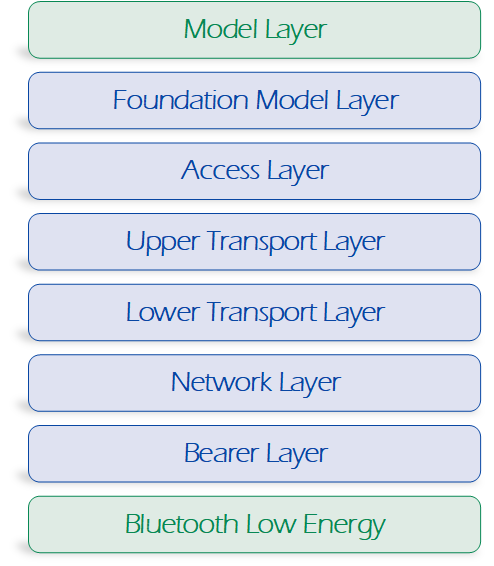
\includegraphics[width = 0.9\textwidth]{images/Layer BLE Mesh.png}
    \caption{Architettura Bluetooth Mesh}
    \label{fig:ble_mesh_architecture}
\end{figure}

\subsection{Bluetooth Mesh Concepts}
% https://docs.espressif.com/projects/esp-idf/en/latest/api-guides/esp-ble-mesh/ble-mesh-terminology.html
Lo standard Bluetooth Mesh \cite{blemesh2017, bluetooth2019b}, anche se eseguito al disopra dello stack BLE, prevede l'impiego di ulteriori concetti finora non appartenenti ad uno standard Bluetooth. Tra cui l'utilizzo del paradigma Publish-Subscribe, l'utilizzo di apposite chiavi di sicurezza per la cifratura dei dati e concetti come quello di elementi e indirizzamento, per citarne alcuni. 
Tali concetti verranno affrontati di seguito.

\subsubsection{Network}
\label{subsub:network}
Una mesh Bluetooth è costituita da dispositivi che cooperano tra di loro e condividono delle risorse, come ad esempio: 
l'\textit{indirizzo di rete} usato per identificare il mittente e il destinatario di un messaggio; % Section 3.4.2
le \textit{chiavi} di \textit{rete} (NetKeys) e di \textit{applicazione} (AppKeys) usate per crittografare e autenticare un messaggio rispettivamente in merito al network layer e access layer.\\ % Section 3.8.6.3 e Section 3.8.6.2
Una rete può essere costituita da una o più sottoreti. Una sottorete racchiude un gruppo di nodi che per comunicare tra loro a livello di rete adottano la medesima network key. Un nodo può essere a conoscenza di una o più Netkeys, il che gli consente di appartenere a più sottoreti.\\
Una rete mesh Bluetooth può essere costituita al massimo da 32767 nodi e la massima distanza che un messaggio può percorrere, espressa in termini di hop, all'interno della rete è di 127 hop.

\subsubsection{Nodi}
\label{subsub:nodi}
Un \textit{nodo} è un dispositivo che si è unito ad una rete mesh Bluetooth. Un dispositivo, prima di entrare a far parte di una tale rete è identificato con il termine \textit{unprovisioned device}. Nel momento in cui entra a farvi parte, a seguito di un processo di \textit{provisioning} che consente di autenticare il dispositivo e comunicargli informazioni di base necessarie per la comunicazione con gli altri nodi appartenenti ad essa, viene identificato con il termine \textit{nodo}. Solo nel momento in cui assume il ruolo di nodo, il dispositivo è in grado di inviare, ricevere o inoltrare i messaggi appartenenti alla rete e può opzionalmente far parte anche di una o più sottoreti.\\
Un nodo all'interno della rete può assumere diversi ruoli in base alle features supportate e abilitate. Gli speciali quattro ruoli definibili (descritti nella sezione \ref{subsub:features}) sono i seguenti: \textit{Relay Node}, \textit{Proxy Node}, \textit{Friend Node} e \textit{Low Power Node}. \\
La procedura di provisioning (discussa in \ref{sec:provisioning}) coinvolge un nodo esterno chiamato Provisioner il cui compito è proprio quello di aggiungere un dispositivo ad una rete mesh.

\subsubsection{Elementi}
\label{subsub:elementi}
% un'entità indirizzabile all'interno di un dispositivo
Un nodo può essere costituito da più parti che possono essere controllate in modo indipendente. Ogni singola entità indirizzabile in modo univoco presente all'interno di un nodo è identificata come \textit{elemento}. Ogni nodo è costituito da almeno un elemento, denominato primary element. Gli altri elementi che costituiscono il nodo sono indicati o come elementi addizionali o come secondary element. Ogni elemento, sia esso primary sia secondary, contiene uno o più modelli e nel caso in cui sono contenuti più modelli, essi non devono essere uguali.\\
L'elemento primary è indirizzabile usando l'indirizzo univoco assegnato al nodo durante il processo di provisioning, mentre gli eventuali elementi addizionali sono raggiungibili utilizzando indirizzi successivi. Attraverso questi indirizzi univoci è possibile identificare all'interno di un nodo, quale elemento sta trasmettendo o ricevendo messaggi.\\
Ad esempio, un lampadario può contenere più lampadine che possono essere accese o spente in modo indipendente, ogni singola lampadina costituisce un elemento del nodo lampadario.

\subsubsection{Stati}
\label{subsub:stati}
Lo \textit{stato} è un valore che rappresenta una condizione di un elemento. Un elemento che espone uno stato è definito \textit{server}, mentre un elemento che accede ad uno stato è definito \textit{client}. Il più semplice esempio di server è un Generic OnOff Server in cui lo stato può essere `on' oppure `off', mentre un Generic OnOff Client è in grado di gestire gli stati di un Generic OnOff Server tramite dei messaggi definiti dal Generic OnOff Server Model.\\
Uno stato può essere cambiato come risultato della ricezione ed elaborazione di specifici messaggi. Il cambiamento da uno stato ad un altro stato è indicato \textit{state transition} e può essere istantaneo o può accadere in un intervallo di tempo. Il tempo impiegato per passare dallo stato attuale a quello appena comunicato viene chiamato \textit{transition time}. Il cambiamento di stato è probabile che provochi un cambiamento nel comportamento dell'elemento. Inoltre, un messaggio può contenere un determinato parametro (delay) che consente di posticipare l'inizio dello state transition di un intervallo temporale descritto da tale parametro.\\

\noindent Gli stati possono essere costituiti da due o più valori, in tal caso sono conosciuti come \textit{stati compositi}. Un esempio può essere una lampada in grado di cambiare colore in cui è possibile scegliere la tonalità del colore separatamente dalla saturazione e dalla luminosità.\\

\noindent Alcuni stati possono essere legati ad altri (\textit{bound states}), questo significa che la variazione di uno stato comporterà un cambiamento anche nell'altro. Un semplice esempio potrebbe essere l'associazione tra uno stato `Level' ed un `OnOff' all'interno di un dimmer per la gestione di una lampadina. Impostando il livello a 0 innescherà una transizione di stato anche per lo stato OnOff, impostato ad `off'. Cambiando il livello in uno stato diverso da 0 innescherà una transizione di stato che assegnerà `on' allo stato OnOff. Questo esempio mostra un'associazione unidirezionale, ma in realtà essa può essere anche bidirezionale, con lo stato OnOff che influenza lo stato Level. Le regole di associazione sono definite esplicitamente nella definizione degli stati.\\

\noindent Un altro concetto molto legato agli stati è quello di \textit{scena}. Una scena è una raccolta di stati ed è identificata da un numero univoco a 16 bit all'interno di una rete. Le scene consentono di attivare un'azione per impostare più stati di nodi diversi. Possono essere innescate on-demand o in un momento specifico. Ad esempio, una scena può essere configurata per impostare la temperatura in una stanza, la luminosità delle luci in un'altra e la chiusura delle persiane in un'altra ancora.

\subsubsection{Messaggi}
\label{subsub:messaggi}
Ogni comunicazione all'interno di una rete mesh è eseguita inviando dei messaggi il cui compito è quello di operare sugli stati. I messaggi sono associati ai modelli e agli stati che definiscono lo status di un elemento. Per ogni stato, esiste un insieme definito di messaggi supportato da un server e utilizzabili da un client per richiedere un valore di uno stato o per settare tale valore.\\
Un messaggio risulta identificato attraverso un opcode (identifica il tipo di operazione del messaggio) a cui corrispondono dei parametri associati i quali consentono di definire un comportamento.\\
Ci sono tre tipi di messaggi in BLE Mesh, ognuno dei quali è definito tramite un opcode (operation code) univoco:
\begin{itemize}
    \item il \textit{GET message} utilizzato per richiedere informazioni in merito al valore di uno stato di un server model. Un messaggio di tipo GET non prevede parametri.
    
    \item il \textit{SET message} utilizzato per modificare il valore di un determinato stato appartenente ad un server model. Questo tipo di messaggio richiede diversi parametri, tra cui il valore da assegnare allo stato, il TID (Transaction Identifier) utilizzato per indicare se si tratta di un nuovo messaggio o la ritrasmissione, il Transition Time usato per indicare la quantità di tempo da impiegare per passare da uno stato all'altro e il Delay per indicare di quanto posticipare l'esecuzione del messaggio.
    
    \item lo \textit{STATUS message} utilizzato in differenti scenari:
    \begin{itemize}
        \item inviato in risposta ad un GET message, contenente il valore dello stato.
        \item inviato in risposta ad un SET message quando è previsto l'uso di acknowledgment.
        \item inviato in modo indipendente per riferire lo stato di un elemento.
    \end{itemize}
\end{itemize}

\noindent Tra i messaggi utilizzati per scambiare informazioni all'interno di una rete mesh, alcuni richiedono un messaggio di riscontro (acknowledgement) da parte di ogni elemento ricevente, mentre altri, denominati unacknowledged non prevedono nessuna formula di risposta alla ricezione di un messaggio. Tale distinzione avviene per i messaggi di tipo SET, in cui l'eventuale risposta avviene  solitamente attraverso uno STATUS message. L'utilizzo di tale ack serve a due scopi:
\begin{itemize}
    \item confermare la ricezione di un messaggio.
    \item ritornare i dati richiesti dal messaggio ricevuto.
\end{itemize}

\noindent Nel caso in cui il messaggio di risposta non venga ricevuto dal mittente, o viene ricevuto una risposta inaspettata, il mittente può decidere di inviare nuovamente il messaggio.\\

\noindent Esistono anche dei messaggi di servizio, chiamati Heartbeat. Questi messaggi sono inviati periodicamente e servono ad indicare agli altri nodi della rete che il mittente è vivo e attivo.

\subsubsection{Indirizzi}
\label{subsub:indirizzi}
All'interno di una rete mesh i nodi comunicano scambiandosi messaggi e per poter individuare mittente e destinatario di una comunicazione è opportuno utilizzare appositi indirizzi. Lo standard Bluetooth Mesh prevede tre tipi di indirizzi:
\begin{itemize}
    \item \textit{Unicast Address}: un indirizzo assegnato durante il processo di provisioning ad un nodo e consente di identificarlo, per tutta la sua permanenza, in modo univoco all'interno di una rete mesh.\\
    In realtà, l'indirizzo unicast è assegnato ad ogni elemento di un nodo e può comparire nel campo indirizzo mittente/destinatario di un messaggio. Il messaggio destinato ad un indirizzo unicast potrà essere processato solo dall'elemento in possesso di tale indirizzo.\\
    All'interno di una rete mesh si possono assegnare al massimo 32767 indirizzi unicast.
    
    \item \textit{Group Address}: è un indirizzo multicast e viene utilizzato per rappresentare un gruppo di nodi, solitamente riflette un raggruppamento fisico di nodi, come ad esempio tutti i nodi presenti in una specifica stanza. \\
    Esistono 16384 group address, di cui 256 sono definiti da Bluetooth SIG con il nome \textit{SIG-Fixed Group Address} e sono utilizzati per identificare tutti gli elementi primari dei nodi distinguendoli in base alle loro funzionalità (All-proxies, All-Friends, All-relays e All-nodes). I restanti 16128 indirizzi sono chiamati \textit{Dynamic Group Address} e sono definiti dall'utente a livello di applicazione.
        
    \item \textit{Virtual Address}: è un indirizzo multicast e consente di rappresentare più elementi o addirittura anche più nodi. Ogni Virtual Address rappresenta logicamente una Label UUID e risulta essere costituita da 128 bit. Tale indirizzo prevede che il bit in posizione 15 e 14 siano impostati rispettivamente ad 1 e a 0, mentre i bit compresi tra la posizione 13 e 0 rappresentano un valore hash (sono disponibili 16384 valori hash). Il valore hash è una derivazione della label UUID ed è stato introdotto per diminuire l'overhead presente nei messaggi e quindi fornire un metodo più efficiente la tipologia di elementi a cui sono destinati tali messaggi. 
\end{itemize}

\noindent In realtà, esiste anche un indirizzo speciale, denominato \textit{Unsigned Address} con valore di $0x0000$ e utilizzato per indicare che un \textit{elemento} non è stato ancora configurato o assegnato l'\textit{Unicast Address}. Gli elementi in possesso del unsigned address non possono essere utilizzati per comunicare poiché risultano non dotati di un indirizzo valido per la comunicazione. Solo dopo aver assegnato loro un unicast address potranno essere utilizzati per la comunicazione.

\subsubsection{Publish-Subscribe}
\label{subsub:publish_subscribe}
All'interno di una rete mesh, per consentire ai nodi di scambiarsi messaggi viene utilizzato il paradigma publish-subscribe.\\
Il processo che consente ad un nodo di generare ed inviare un messaggio ad uno o più dispositivi viene definito \textit{Publishing}. La configurazione adottata da un nodo interessato ad elaborare messaggi inviati ad indirizzi specifici è nota come \textit{Subscribing} e prevede una sottoscrizione a questi indirizzi (memorizzati nella \textit{subscriber list}). I messaggi possono essere destinati o ad un unicast address o pubblicati attraverso un group address o un virtual address.\\

\noindent I nodi possono pubblicare unsolicited messages o messaggi in risposta ad altri messaggi.\\
Quando un nodo invia un messaggio di risposta, utilizza come indirizzo di destinazione l'indirizzo del mittente originario.\\
Gli unsolicited messages possono essere pubblicati utilizzando come indirizzo di destinazione, definito publish address, uno tra i seguenti indirizzi: unicast, pre-configured group, virtual. Ogni modello all'interno di un nodo ha un singolo publish address.\\

\noindent Lato ricezione, ogni istanza di un modello per ricevere messaggi può sottoscriversi ad uno o più indirizzi group o virtual. Ogni volta che viene pubblicato un messaggio sugli indirizzi group o virtual a cui il modello risulta essere iscritto, verrà elaborato dal nodo. Un messaggio viene elaborato anche quando l'indirizzo di destinazione corrisponde ad un indirizzo unicast di un elemento appartenente al dispositivo.\\
Un nodo può avere più sottoscrizioni per ogni singola istanza del modello di un elemento. In tal modo si consente al nodo di ricevere i messaggi pubblicati in differenti gruppi. Di seguito un semplice esempio di rete mesh all'interno di un'abitazione composta da 6 interruttori e 9 lampadine. 

\begin{figure}[!ht]
    \centering
    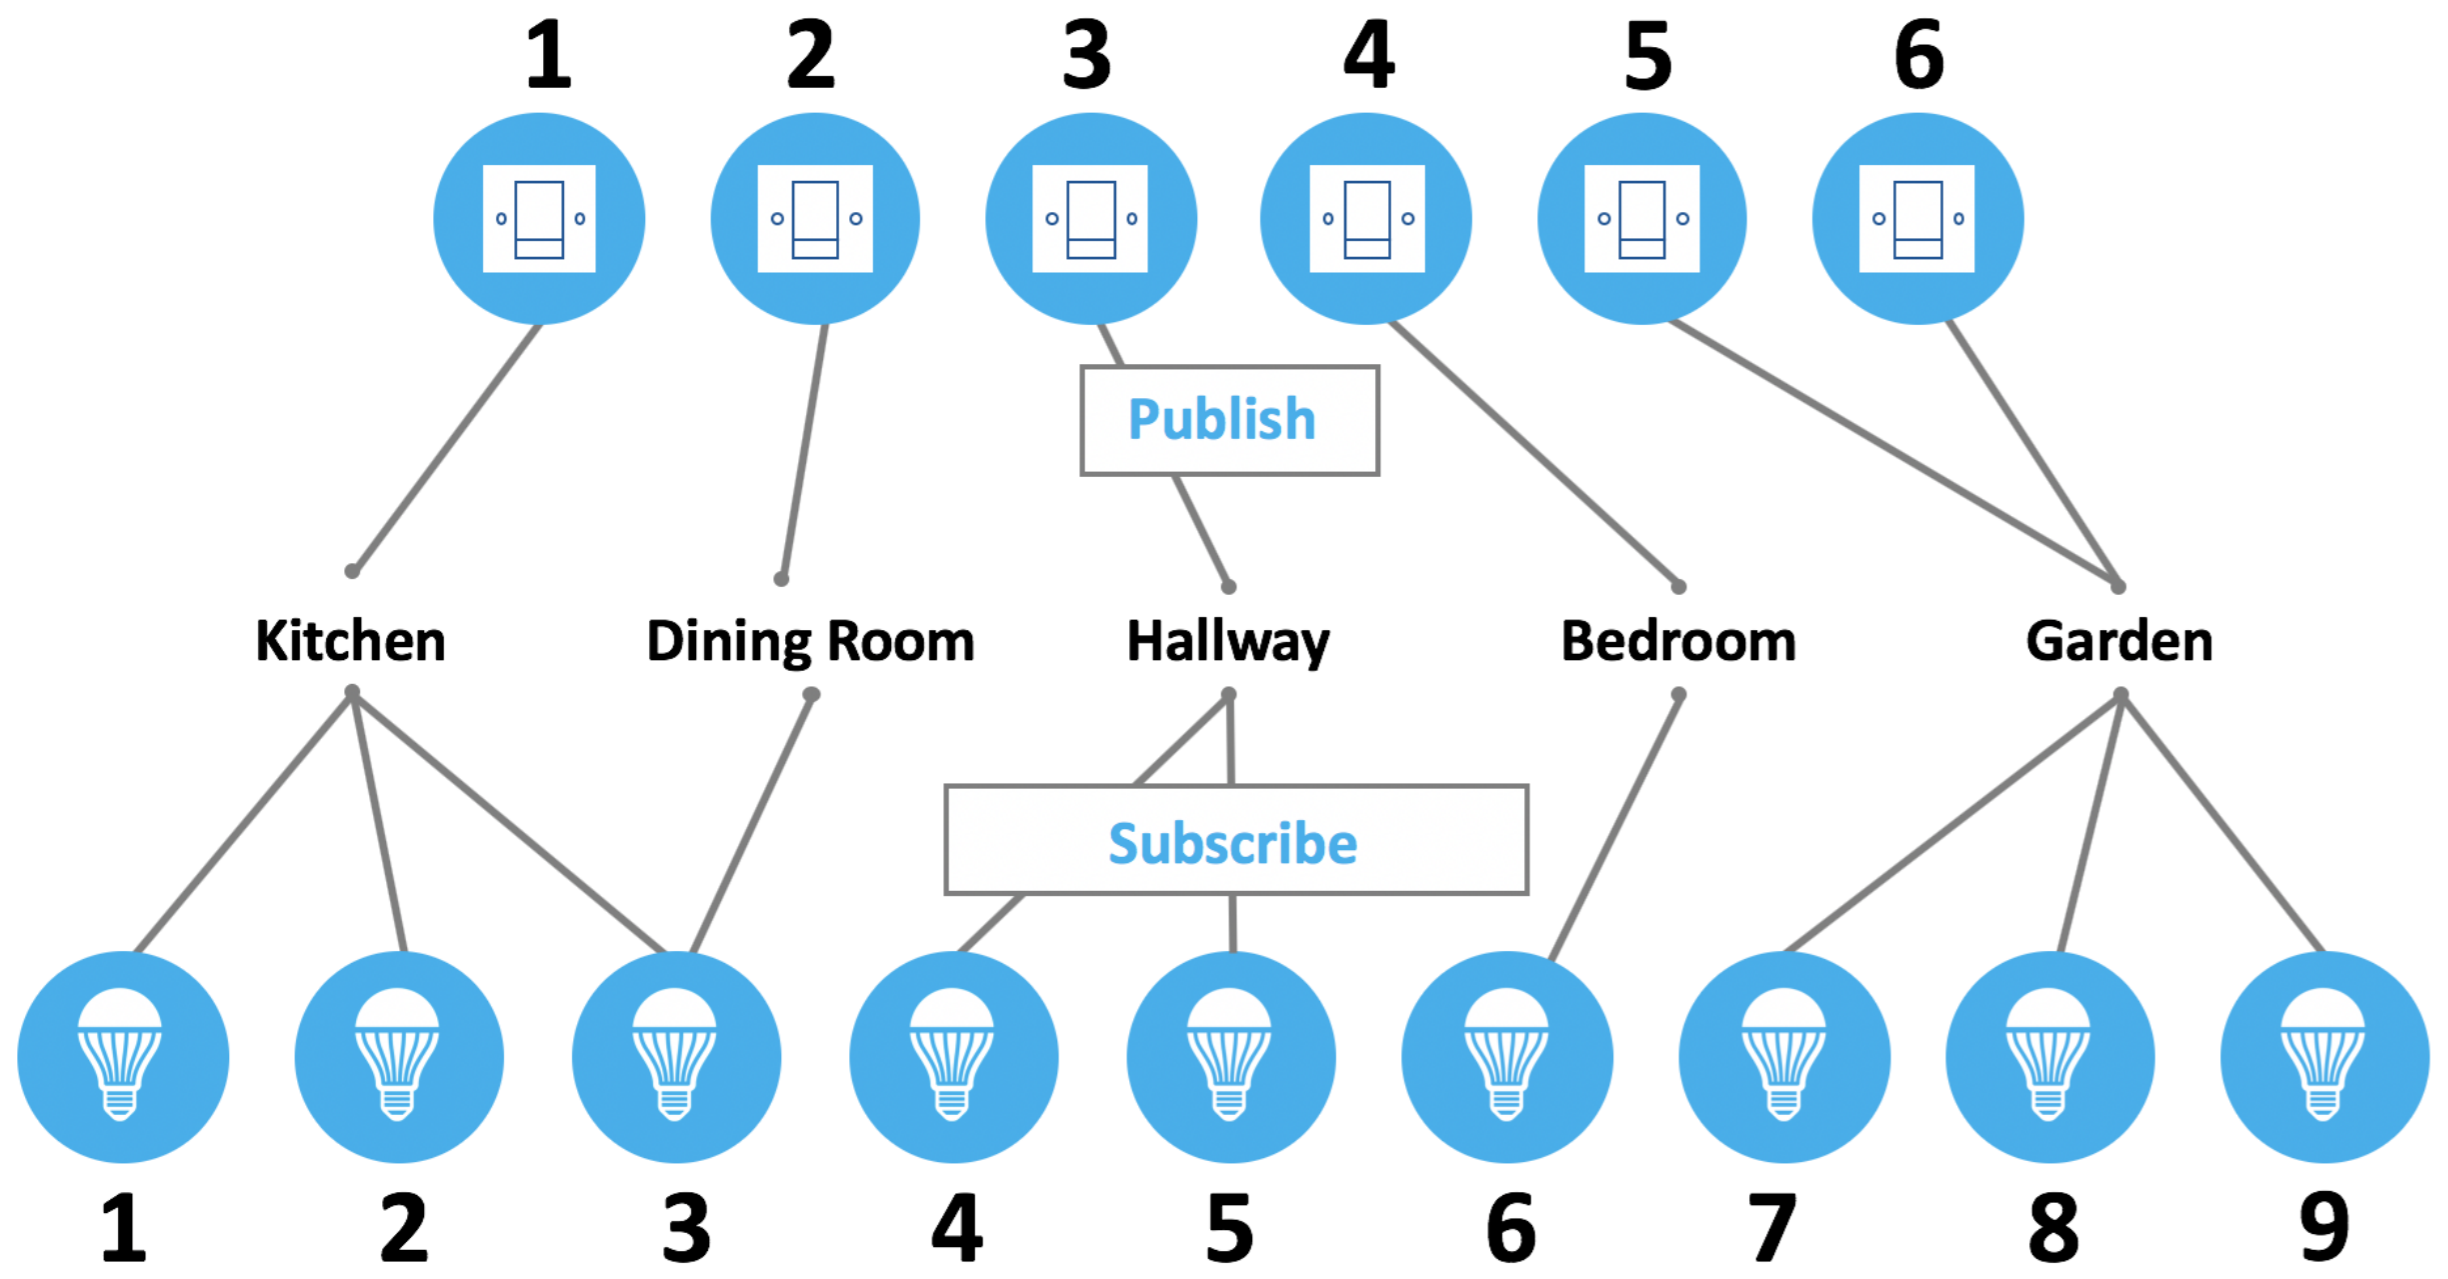
\includegraphics[width = \textwidth]{images/Publish_Subscribe_BLE.png}
    \caption{Esempio Publish-Subscribe}
    \label{fig:publish_subscribe_ble}
\end{figure}

\noindent La figura \ref{fig:publish_subscribe_ble} è un tipico esempio di come una lampadina (\#3) può essere sottoscritta a più indirizzi (Kitchen e Dining Room) e come più interruttori (\#5 e \#6) possono gestire lo stesso ambiente (Garden). Utilizzando group o virtual address, aggiungere o rimuovere i nodi non comporta alcuna riconfigurazione degli altri nodi.\\

\noindent Ogni messaggio viene inviato da un singolo unicast address e identificato utilizzando un numero di sequenza univoco per facilitare il rilevamento e fronteggiare i possibili attacchi che prediligono la riproduzione di un messaggio.



\subsubsection{Managed Flooding}
\label{subsub:managed_flooding}
La comunicazione all'interno di una rete Mesh avviene tramite un meccanismo di flooding che prende il nome di \textit{Managed Flooding}. Tale tecnica utilizza i canali advertising per trasmettere messaggi in modo che gli altri nodi possano riceverli ed eventualmente ritrasmetterli, estendendo così la portata del messaggio originario. 
Senza una corretta gestione, il meccanismo di flooding, il quale prevede che ogni nodo debba ritrasmettere i messaggi ricevuti finché non viene raggiunto il nodo di destinazione, ridurrebbe gravemente la scalabilità, la robustezza della rete. %Un aspetto da non sottovalutare utilizzando un meccanismo di flooding è la possibilità di intasare la rete con messaggi superflui.
A tal proposito, il meccanismo adottato per le operazioni di routing all'interno di una rete Bluetooth Mesh prevede dei metodi per limitare il processo di inoltro, come: \textit{network message cache} e \textit{time to live}. In più tale standard consente di definire quali nodi debbano svolgere il ruolo di \textit{relay node}.\\
Il metodo network message cache è progettato per impedire ai dispositivi di inoltrare più volte il medesimo messaggio e, per tenerne traccia dei messaggi che sono stati già inviati, ogni messaggio ricevuto viene memorizzato in cache andando a creare una sorta di lista. In tal modo, ogni volta che viene ricevuto un messaggio, viene confrontato con questo elenco e se già presente il lista il messaggio viene ignorato, altrimenti si procede ad inoltrarlo e aggiungerlo alla lista. Operando in questo modo, con il crescere dei messaggi gestiti dal nodo, si potrebbe giungere ad avere un elenco infinito, difatti per evitare ciò, il numero di messaggi memorizzati in cache è limitato e può essere impostato tramite un apposito parametro in fase di configurazione del nodo.\\
Time to live (TTL) è un valore presente all'interno di ogni messaggio e limita il numero di volte che esso può essere inoltrato all'interno della rete. Ogni qualvolta che un messaggio viene ricevuto e poi inoltrato (fino ad un massimo di 126 volte), il valore TTL viene decrementato di 1. Nel momento in cui tale campo assume valore 0, il messaggio non potrà essere inoltrato, quindi verrà scartato.\\
Quindi, un relay node procederà ad inoltrare un messaggio solo se non è presente in cache e solo se il suo TTL è maggiore di 1.

\subsubsection{Modelli}
\label{subsub:modelli}
Il \textit{modello} implementa e definisce le funzionalità di base di un determinato nodo, ovvero provvede a definire gli stati, i messaggi che agiscono su di essi e qualsiasi comportamento associato a seguito di una transazione.\\
Un nodo può contenere molteplici modelli e ognuno di essi determina le funzionalità dell'elemento cui si riferisce.\\
Tutte le comunicazioni all'interno di una rete Bluetooth sono eseguite per mezzo di messaggi i quali sono definiti come parte della specifica di un modello. Lo standard prevede tre categorie di modelli: client, server e control model.

\begin{itemize}
    \item un \textit{Server model} è composto da uno o più stati estesi tra uno o più elementi. Tale modello supporta appositi messaggi per operare sul comportamento relativo all'elemento o per comunicare il suo valore.
    
    \item un \textit{Client model} definisce un insieme di messaggi che il client usa per richiedere, modificare o utilizzare gli stati del server corrispondente, così come definito dal server model adottato. Il client model non ha stati.
    
    \item un \textit{Control model} può contenere sia le funzionalità di un client model sia le funzionalità di un server model per comunicare rispettivamente con altri server model o con altri client model.
\end{itemize}
Un singolo dispositivo può contenere anche tutti e tre i modelli appena descritti. 
Un modello, per includere funzionalità addizionali che gli consentono di gestire determinati comportamenti, deve essere obbligatoriamente esteso, anche perché tali oggetti risultano immutabili, vale a dire che non è permesso modificarne uno aggiungendo o rimuovendo un comportamento.
Un modello che non estende altri moduli è chiamato \textit{root model}.\\
L'implementazione delle funzionalità dei nodi avviene attraverso i modelli, che possono essere divisi in SIG Model e Vendor Model, rispettivamente definiti da Bluetooth SIG e dai fornitori dei dispositivi o dagli utenti. In entrambi i casi, i modelli risultano identificabili attraverso un identificativo univoco di 16 bit per quelli SIG e 32 bit per quelli Vendor.

\subsubsection{Features}
\label{subsub:features}
Tutti i nodi hanno l'abilità di trasmettere e ricevere i messaggi. Tuttavia, le funzionalità di un nodo sono determinate dalle caratteristiche che esso supporta. I nodi possono supportare nessuna, una o più caratteristiche addizionali, abilitate o disattivate in qualsiasi momento:
\begin{itemize}
    \item \textit{Relay} feature: l'abilità di ritrasmettere quei messaggi inviati in broadcast dagli altri nodi. 
    Ciò consente di estendere la portata di ogni singolo messaggio e fare in modo che possa attraversare l'intera rete con lo scopo di raggiungere anche tutti quei nodi non direttamente connessi al mittente. Con l'introduzione di questa caratteristica si ha la possibilità di creare una rete di grosse dimensioni.\\ % Managed Flooding
    Un nodo che supporta ed ha attiva tale funzionalità è definito come \textit{Relay node}.\\
    Il Relay node si preoccupa di inoltrare solo quei messaggi appartenenti alla propria sottorete. Nel caso di segmentazione del messaggio, il nodo provvederà ad inoltrare ogni singolo segmento una volta ricevuto, anziché attendere il messaggio completo.
    
    \item \textit{Proxy} feature: l'abilità di ricevere e ritrasmettere i messaggi tra GATT e advertising bearer. \\
    Tale caratteristica garantisce la retrocompatibilità per quei dispositivi BLE che non supportano Bluetooth mesh. In questo modo, un dispositivo BLE nativo come uno smartphone può anche comunicare con i dispositivi appartenenti ad una rete mesh. 
    In tale circostanza si ha un dispositivo connection-oriented con il nodo proxy e quest'ultimo tramite le operazioni messe a disposizione dallo standard BLE (operazioni GATT) è in grado di agire da intermediario e quindi consentire a questa tipologia di dispositivi ad interfacciarsi ed interagire con i nodi appartenenti alla rete mesh.\\
    Quindi, attraverso la seguente funzionalità il nodo è in grado di eseguire una traduzione tra le PDU proxy e le PDU mesh. Il nodo che supporta ed ha attiva tale funzionalità è conosciuto \textit{Proxy node}.
    
    \item \textit{Low Power} feature: la capacità di operare all'interno di una rete mesh con un duty cycle significativamente ridotto. La sua presenza all'interno di una rete mesh è resa possibile solo in combinazione con un nodo che supporta la relazione ``Friendship''.\\
    Un nodo che supporta tale funzionalità ed ha attiva un'amicizia con un Friend node è definito \textit{Low Power node} e tramite un meccanismo di polling ottiene informazioni dal suo Friend node.
    
    \item \textit{Friend} feature: la capacità di supportare un Low Power node, difatti è responsabile della memorizzazione dei messaggi destinati ai suoi nodi ``amici'' e dell'inoltro di messaggi generati da questi nodi all'interno della rete. A tal proposito ogni nodo amico dovrebbe essere anche un nodo relay.\\
    Un nodo che supporta ed ha attiva tale funzionalità, ed inoltre ha un'amicizia con un Low Power node è definito \textit{Friend node}. L'aver abilitato la funzionalità Friend può comportare un maggior consumo energetico, a tal proposito questi nodi risultano, molto spesso, essere alimentati tramite la rete elettrica.
\end{itemize}

\paragraph{Friendship}
Friendship è una speciale relazione tra un \textit{Low Power node} e un \textit{Friend node} che consente la presenza del primo all'interno di una rete mesh. Tale relazione consente al nodo con poche risorse energetiche di limitare la quantità di tempo in cui debba essere in ascolto e soprattutto consente di evitare la perdita di messaggi ad esso destinati. Affinché sia attuabile tale relazione questi due tipi di nodi devono essere adiacenti, ovvero trovarsi ad un singolo hop di distanza e nella medesima sottorete.\\

\noindent Il nodo Low Power solitamente ha un'alimentazione limitata (a batteria) e provvede a risparmiare energia mantenendo la radio spenta il più possibile, garantendo così un ridotto duty cycle. Il nodo periodicamente si sveglia per eseguire delle interazioni con il nodo amico per poi tornare nuovamente in sleep mode. Le interazioni prevedono il polling dal nodo Friend per recuperare i messaggi ad esso destinati e se necessario procede con l'invio di messaggi ai nodi della rete.\\
Il nodo Low Power necessita di un nodo Friend per poter stabilire tale relazione, infatti la procedura che consente di giungere in questo stato è avviata proprio dal nodo Low Power. Una volta stabilita la relazione, il nodo Friend esegue una serie di azioni che aiutano a ridurre il consumo di energia al nodo a bassa potenza permettendogli di programmare la frequenza appropriata per l'impiego della propria radio e quindi l'operazione di polling per verificare la presenza di nuovi messaggi ad esso destinati.\\
Il nodo Friend utilizza una Friend Queue per memorizzare tutti i messaggi in arrivo indirizzati ai propri nodi amici e provvede a recapitarli quando richiesto da tali nodi. Inoltre, garantisce anche supporto in merito agli aggiornamenti relativi alla sicurezza per i suoi nodi amici.\\
Una volta che la relazione è stabilita tra i due nodi, essi sono considerati ``friends''. Un nodo Friend può essere amico con più nodi Low Power, mentre un nodo Low Power può avere un unico Friend node.\\

\noindent Solitamente i nodi Low Power sono dei semplici sensori che si occupano di inviare periodicamente la lettura del valore acquisito in broadcast nella rete e non sono soggetti alla ricezione di molti messaggi. Gli unici messaggi che solitamente ricevono riguardano la configurazione di determinate soglie, come ad esempio l'intervallo di tempo con cui il nodo deve inviare i dati acquisiti.

\paragraph{Mesh Gateway}
Un mesh gateway è quel nodo in grado di tradurre i messaggi tra una rete mesh e una tecnologia non Bluetooth.

\section{Provisioning}
\label{sec:provisioning}
% %.4.2 Provisioning behavior
% https://www.bluetooth.com/blog/provisioning-a-bluetooth-mesh-network-part-1/
% https://www.bluetooth.com/blog/provisioning-a-bluetooth-mesh-network-part-2/
Il processo di provisioning è uno dei concetti più importanti in BLE Mesh. Consente, mediante uno scambio di informazioni tra un unprovisioned device ed un provisioner, di aggiungere il dispositivo all'interno di una rete mesh. Il processo è gestito da un provisioner, in genere uno smartphone o un altro dispositivo di elaborazione mobile in grado di eseguire un'applicazione di provisioning.\\
La specifica Bluetooth mesh definisce il protocollo di provisioning ed il suo funzionamento. Per eseguire tale procedura sono state definite apposite PDU, necessarie per comunicare tra un provisioner ed un nuovo dispositivo che desidera entrare a far parte di una rete mesh.

\begin{figure}[!ht]
    \centering
    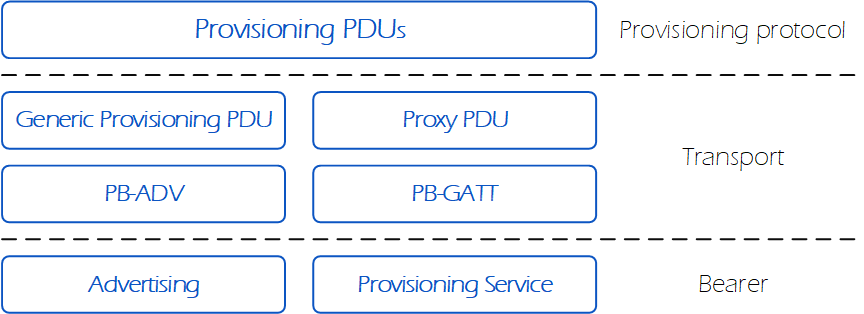
\includegraphics[width = \textwidth]{images/Provisioning_architecture.png}
    \caption{Provisioning protocol stack}
    \label{fig:provisioning_stack}
\end{figure}

\begin{itemize}
    \item il \textit{Provisioning Bearer} layer consente il trasporto di apposite PDU tra il provisioner e un unprovisioned device, definendo due tipologie di Bearer:
    \begin{itemize}
        \item \textit{PB-ADV}: una tecnica di provisioning bearer utilizzata per eseguire la procedura di provisioning di un dispositivo sfruttando i canali advertising. Il PB-ADV bearer è utilizzato per trasmettere Generic Provisioning PDU.\\
        Un dispositivo che supporta PB-ADV dovrebbe eseguire la scansione passiva con un duty cycle vicino al 100\% per evitare di perdere qualsiasi Generic Provisioning PDU in arrivo.
        
        \item \textit{PB-GATT}: un provisioning bearer che consente ad un dispositivo che non supporta PB-ADV di comunicare indirettamente con i nodi di una rete mesh incapsulando i Provisioning PDU all'interno di proxy PDU avvalendosi di un proxy node. Il protocollo proxy consente ai nodi di inviare e ricevere network PDU, mesh beacon, messaggi di configurazione proxy e provisioning PDU avvalendosi di una connessione orientata eseguita utilizzando lo standard BLE (canali Data).
    \end{itemize}
    
    \item il \textit{Provisioning Protocol} definisce i requisiti in merito alle PDU, comportamento e sicurezza. Sono state definite 10 provisioning PDU: Provisioning Invite, Provisioning Capabilities, Provisioning State, Provisioning Public Key, Provisioning Input Complete, Provisioning Confirmation, Provisioning Random, Provisioning Data, Provisioning Complete, Provisioning Failed.
\end{itemize}

\noindent La procedura di provisioning deve svolgere due importanti compiti di alto livello:
\begin{enumerate}
    \item autenticare l'unprovisioned device. L'autenticazione viene eseguita per assicurare che il dispositivo con cui interagisce il provisioner sia il dispositivo che l'utente vuole far subentrare nella rete mesh.
    
    \item creare un collegamento sicuro tra i due dispositivi e procedere con la condivisione delle informazioni, tra cui la chiave di rete e l'indirizzo unicast per ogni elemento presente nel nodo.
\end{enumerate}

\subsection{Provisioning Procedure}
La procedura di provisioning prevede cinque fasi: Beaconing, Invitation, Exchange public keys, Authentication e Distribution of provisioning data.

\subsubsection{Beaconing}
Un dispositivo che vuole subentrare all'interno di una rete mesh e supporta \textit{PB-ADV}, pubblicizza la propria presenza inviando in broadcast di appositi pacchetti (Unprovisioned Device Beacon) sui canali di advertising.\\
Quando viene usato PB-GATT da un unprovisioned device, la procedura di provisioning e le interazione con il provisioner sono supportate da un servizio GATT chiamato Mesh Provisioning Service. Nella fase di Beaconing il dispositivo che vuole entrare a far parte della rete trasmette in broadcast pacchetti pubblicitari contenenti l'UUID del Mesh Provisioning Service e viene individuato dal provisioner tramite la procedura di scansione dello standard BLE. 
Con tale fase, il dispositivo indica al provisioner la disponibilità ad avviare il processo di provisioning.

\subsubsection{Invitation}
Dopo la fase di Beaconing, il provisioner e l'unprovisioned device stabiliscono una provisioning bearer, vale a dire che il provisioner individua i beacon inviati sui canali advertising e provvederà ad inviare un Provisioning Invite PDU al nuovo dispositivo, il quale si appresterà a rispondere tramite un Provisioning Capabilities PDU.

\begin{figure}[!ht]
    \centering
    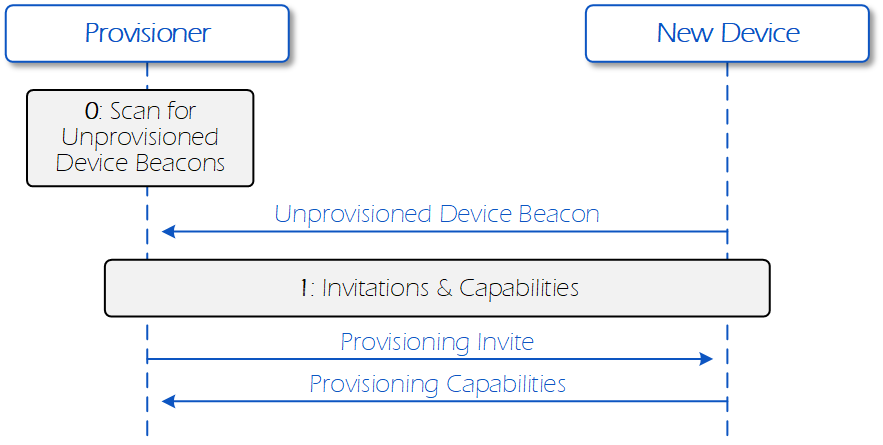
\includegraphics[width = \textwidth]{images/Provisioning_Invitation.png}
    \caption{Provisioning Invitation}
    \label{fig:provisioning_invitation}
\end{figure}

\noindent La fase descritta dalla figura \ref{fig:provisioning_invitation} ha l'obiettivo di fornire al provisioner le informazioni in merito alle capacità supportate dal device e in base a ciò verrà decisa la modalità utilizzata per eseguire la procedura di provisioning.\\

\noindent Il Provisioning Invite PDU include un campo Attention Duration che indica per quanto tempo l'elemento primario del unprovisioned device deve attirare l'attenzione dell'utente usando l'Attention Timer, una qualche forma di indicazione visiva.\\
Il Provisioning Capabilities PDU include:
\begin{itemize}
    \item il numero di elementi supportati dal dispositivo.
    \item l'insieme degli algoritmi di sicurezza supportati.
    \item la disponibilità della sua public key utilizzando il metodo Out-of-Band (OOB).
    \item la capacità del dispositivo di fornire un valore in output all'utente.
    \item la capacità di un dispositivo di ricevere in input un valore dall'utente.
\end{itemize}

\subsubsection{Exchange public keys}
% https://www.bluetooth.com/blog/provisioning-a-bluetooth-mesh-network-part-1/
Questa fase riguarda un aspetto di sicurezza e prevede la combinazione di due tecniche di crittografia per scambiare delle informazioni in modo sicuro: cifratura simmetrica (crittografia a chiave segreta) e cifratura asimmetrica (crittografia a chiave pubblica).

\begin{itemize}
    \item la \textit{cifratura Simmetrica} utilizza la stessa chiave segreta sia per la cifratura che per la decifratura. Nel momento che mittente e destinatario conoscono la chiave segreta, possono decrittografare tutti i messaggi crittografati con tale chiave. La problematica di tale procedura riguarda lo scambio in totale sicurezza della chiave segrete su un collegamento e impedire che cadano in mani sbagliate.

    \item la \textit{cifratura asimmetrica} utilizza due chiavi correlate proprio per risolvere il problema sopra citato: chiave pubblica e chiave privata. Qualsiasi messaggio viene cifrato utilizzando la chiave pubblica e può essere decifrato solo applicando lo stesso algoritmo e la chiave privata corrispondente. Tuttavia, questa tecnica è più lenta della precedente e richiede molta più potenza di elaborazione per crittografare e decrittografare il contenuto dei messaggi.
\end{itemize}

\noindent Poiché la tecnica asimmetrica risulta essere computazionalmente costosa per i dispositivi coinvolti e poiché la tecnica simmetrica non garantisce uno scambio di chiavi in modo sicuro, Bluetooth Mesh utilizza una combinazione di metodi simmetrici e asimmetrici per fronteggiare tale problematica.\\
Tale combinazione prevede l'utilizzo dell'Elliptic-curve Diffie-Hellman (ECDH), un protocollo che consente a due parti, ognuna con una coppia di chiavi elliptic curve pubblica-privata, di stabilire un segreto condiviso su un canale non sicuro. Lo scopo di tale algoritmo durante la fase di provisioning riguarda la creazione di un collegamento sicuro tra il provisioner e l'unprovisioned device. Prevede l'uso di chiavi pubbliche e private per distribuire una chiave simmetrica che le due entità potranno utilizzare per crittografare e decrittografare i successivi messaggi trasmessi all'interno di una rete mesh, attraverso la tecnica di crittografia AES-128.\\

\noindent Nella fase di Exchange public keys a seconda delle capacità del dispositivo, scoperte nella fase precedente, il provisioner sceglie la modalità con cui scambiare le chiavi pubbliche ECDH. Lo scambio può avvenire tramite un normale collegamento Bluetooth o tramite la tecnologia OOB.
Dopo aver scelto la metodologia, informa il device tramite l'invio di un Provisioning Start PDU contenente l'approccio da adottare.\\

\noindent Se lo scambio di chiavi pubbliche non è possibile tramite la tecnologia OOB, esso avverrà direttamente tramite un collegamento Bluetooth. Per ogni scambio, una nuova coppia di chiavi deve essere generata sia dal provisioner sia dall'unprovisioned device.

\begin{figure}[!ht]
    \centering
    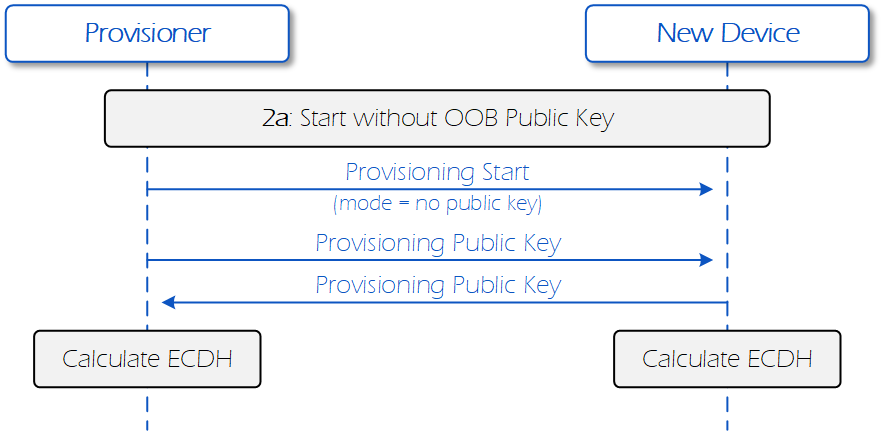
\includegraphics[width = \textwidth]{images/Provisioning_public_key_exchange_a.png}
    \caption{Public Key Exchange dell'unprovisioned device qualora sia sconosciuta}
    \label{fig:provisioning_public_key_a}
\end{figure}

\noindent Altrimenti, se è possibile scambiare la chiave pubblica attraverso il meccanismo OOB, una nuova coppia di chiavi verrà generata solo dal Provisioner e la chiave pubblica relativa verrà trasmessa al dispositivo, il quale sarà in grado di leggere una chiave pubblica statica utilizzando il meccanismo OOB.\\

\begin{figure}[!ht]
    \centering
    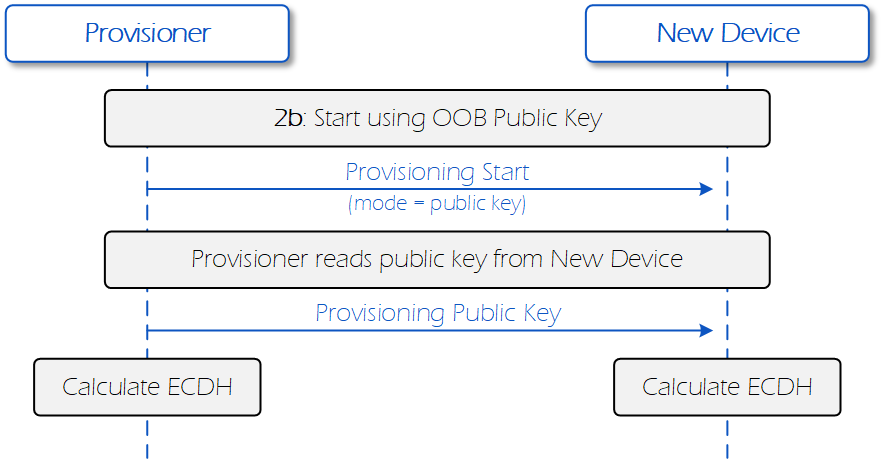
\includegraphics[width = \textwidth]{images/Provisioning_public_key_exchange_b.png}
    \caption{Public Key Exchange tramite il metodo OOB}
    \label{fig:provisioning_public_key_b}
\end{figure}

\noindent I dispositivi coinvolti dovranno verificare se la chiave pubblica ottenuta risulti valida. Se la chiave non è valida il processo di provisioning fallisce. Dopo che la chiave pubblica è nota ed è stata convalidata, ogni dispositivo calcola una chiave simmetrica, nota come ECDHSecret, utilizzando la propria chiave privata e la chiave pubblica del dispositivo peer. Questa chiave verrà utilizzata per proteggere la comunicazione tra i dispositiva da questo punto in avanti.\\
Dopo aver calcolato ECDHSecret, i due dispositivi dovranno eliminare la coppia di chiavi pubblica-privata generate in precedenza.

\subsubsection{Authentication}
% https://www.bluetooth.com/blog/provisioning-a-bluetooth-mesh-network-part-2/
Il prossimo step prevede l'autenticazione del dispositivo. In questo step, il provisioner utilizzerà il metodo di autenticazione selezionato (in base alle capacità del dispositivo) e comunicato al dispositivo all'interno del Provisioning Start PDU. Esistono quattro approcci disponibili: Output OOB, Input OOB, Static OOB e No OOB. Solitamente richiede un'azione da parte dell'utente, il quale dovrà interagire sia con il dispositivo provisioner sia con l'unprovisioned device.

\paragraph{Output OOB}
Se si seleziona il metodo Output OOB, l'unprovisioned device genera un numero casuale e lo mostra all'utente in base alle sue capacità (se fosse una lampadina potrebbe lampeggiare un determinato numero di volte). Tale numero dovrà essere inserito dall'utente sul dispositivo in grado di supportare un'applicazione di provisioning e tal modo il provisioner potrà autenticare il dispositivo. \\
Il processo di autenticazione continua con l'operazione di \textit{check confirmation value}.

\begin{figure}[!ht]
    \centering
    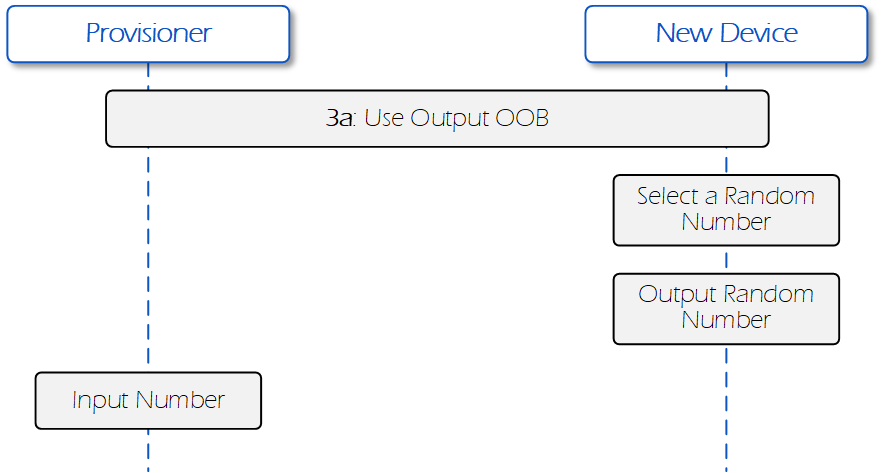
\includegraphics[width = \textwidth]{images/Provisioning_OOB_output.png}
    \caption{Autenticazione con Output OOB}
    \label{fig:provisioning_output_OOB}
\end{figure}

\paragraph{Input OOB}
Il seguente metodo è simile al precedente, ma prevede un'inversione dei ruoli. Il provisioner genera e mostra un numero casuale, dopodiché richiede all'utente di inserirlo nell'unprovisioned device mediante un'azione appropriata e supportata da quest'ultimo.\\
Dopo aver completato l'autenticazione, il dispositivo provvede a comunicare al provisioner, tramite un Provisioning Input Complete PDU, l'avvenuto inserimento del numero casuale. Il processo continua con il \textit{check confirmation value}.

\begin{figure}[!ht]
    \centering
    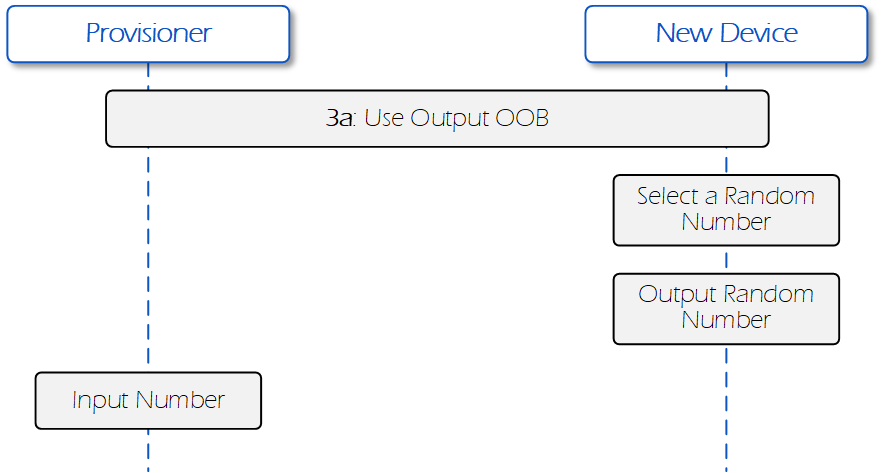
\includegraphics[width = \textwidth]{images/Provisioning_OOB_output.png}
    \caption{Autenticazione con Input OOB}
    \label{fig:provisioning_input_OOB}
\end{figure}

\paragraph{Static OOB o No OOB}
Nel caso in cui non è possibile scegliere i due metodi sopra menzionati, si ricorre all'autenticazione Static OOB o all'autenticazione No OOB.
In ogni caso, ognuno dei due dispositivi genera un numero e si procede con l'operazione di \textit{check confirmation value}, senza la necessità dell'interazione da parte dell'utente. \\
Nel caso della tecnica Static OOB si ricorre all'uso di un valore statico per autenticare il dispositivo. Nel caso della tecnica No OOB si utilizza il valore 0 nel campo relativo allo Static OOB. Utilizzare quest'ultima tecnica è come non autenticare il dispositivo.

\paragraph{Check confirmation value}
L'operazione prevede in primo luogo di calcolare in modo indipendente, per ciascun device, un valore di conferma, conosciuti come \textit{ConfirmationProvisioner} e \textit{ConfirmationDevice} e dopodiché la validazione del valore da parte dell'altro dispositivo. La funzione di generazione del valore di conferma richiede otto parametri i cui valori provengono dalle fasi del processo di provisioning.

\begin{figure}[!ht]
    \centering
    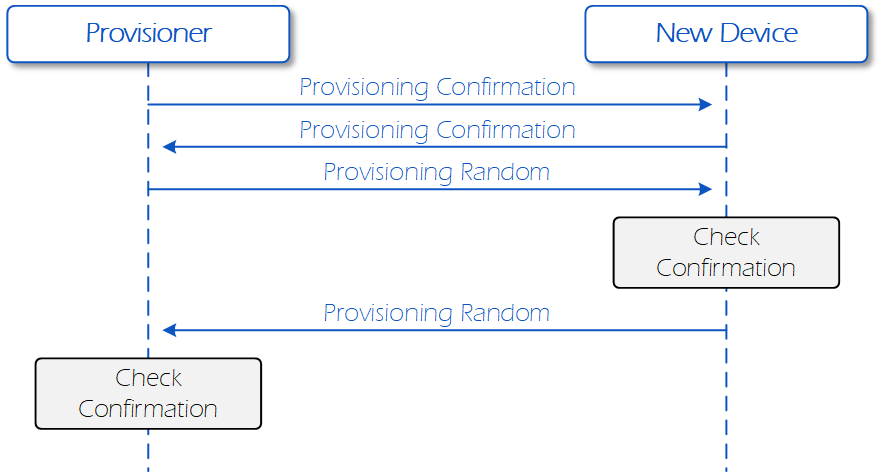
\includegraphics[width = \textwidth]{images/Provisioning_confirmation_value_check.png}
    \caption{Check confirmation value}
    \label{fig:provisioning_confirmation_value_check}
\end{figure}

\noindent Quando i valori di conferma risultano generati, i due dispositivi si scambiano tale informazione e ciascuno controlla l'integrità del valore ricevuto.\\
Il processo di conferma inizia con il provisioner che invia un valore casuale (RandomProvisioner) al peer e quest'ultimo tramite tale valore ricalcola il valore di conferma e lo verifica con il ConfirmationProvisioner. Se non c'è corrispondenza tra i due valori, il processo di provisioning viene interrotto. Altrimenti, il device procede con l'invio di un numero casuale (RandomDevice) al provisioner.\\
Il provisioner, a questo punto, usa lo stesso processo per ricalcolare il valore di conferma e lo verifica confrontandolo con il valore ricevuto in precedenza. Se il valore calcolato non corrisponde al ConfirmationDevice, il processo sarà interrotto. Altrimenti, vorrà dire che l'autenticazione avrà esito positivo e il dispositivo potrà diventare un membro della rete mesh.

\subsubsection{Distribution of provisioning data}
Una volta completata la fase di autenticazione si procede alla fase più importante della procedura: derivazione e distribuzione dei provisioning data. Il provisioner è responsabile della generazione di tali dati, che consistono in una serie di elementi, tra cui la Network Key, la Device Key, un parametro di sicurezza conosciuto come IV index e l'Unicast Address che viene assegnato al dispositivo da parte del provisioner.\\
Per distribuire i ``provisioning data'' in modo sicuro, il provisioner utilizza l'algoritmo AES-CCM per crittografare tali dati con una SessionKey, che entrambi i dispositivi dovranno calcolare. La session Key verrà derivata da ciascun dispositivo usando la propria chiave privata e la chiave pubblica ricevuta dall'altro dispositivo. Una volta calcolata, il povisioner si appresta a cifrare ed inviare la Provisioning Data PDU. 
Dopo aver ricevuto i dati dal Provisioner, il dispositivo dovrà decriptarli (usando la Session Key) e autenticarli. A termine di queste due operazioni, provvederà ad impostare i vari parametri (tra cui la network key e l'unicast address). Al completamento della procedura che assegna l'indirizzo unicast, il dispositivo risponderà al Provisioner con una  Provisioning Complete PDU per confermare l'esito positivo della procedura.

\begin{figure}[!ht]
    \centering
    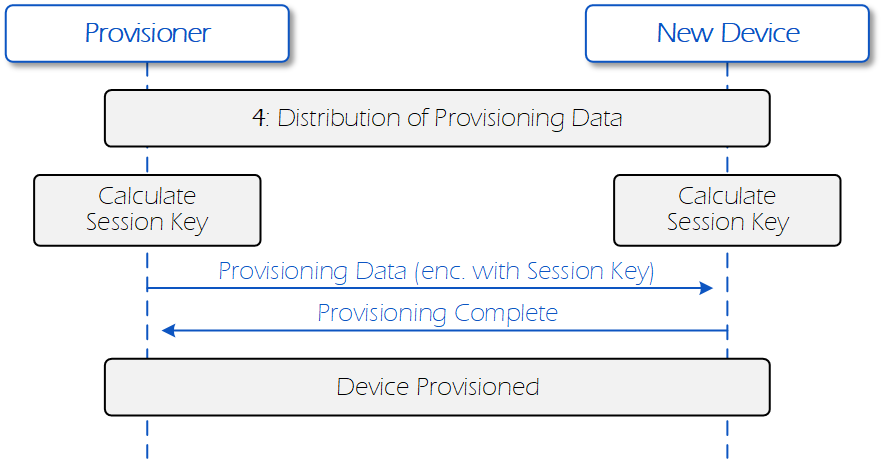
\includegraphics[width = \textwidth]{images/Provisioning_distribution_data.png}
    \caption{Distribution of provisioning data}
    \label{fig:provisioning_distribution_data}
\end{figure}

Con quest'ultimo passaggio, che sancisce la terminazione della procedura di provisioning, l'unprovisioned device diventerà un membro della rete mesh e potrà essere definito \textit{nodo}.

\section{Security}
% https://www.novelbits.io/bluetooth-mesh-tutorial-part-3/
Un aspetto molto importante in Bluetooth Mesh riguarda la sicurezza, rispetto a BLE in cui la sicurezza è facoltativa e la scelta di includerla o meno viene lasciata allo sviluppatore, in Bluetooth Mesh è obbligatoria.\\
Lo standard Bluetooth Mesh prevede che tutti i messaggi all'interno di una rete mesh devono essere crittografati e autenticati tramite apposite chiavi di sicurezza, gestite in modo indipendente dall'upper transport layer e dal network layer. \\
Conservando le due chiavi in modo distinto consente di poter distinguere messaggi con contenuti sensibili (controllo dell'accesso ad un edificio) da messaggi non sensibili (luci di un'abitazione) e consentendo così l'inoltro di un messaggio a qualsiasi nodo della rete (tramite la chiave di rete) senza dover conoscere la chiave di applicazione (non avendo la possibilità di accedere ai dati del livello applicativo).\\

\noindent Il modello di sicurezza definisce due principali chiavi di sicurezza: la chiave del livello di rete (NetKey) e la chiave del livello applicativo (AppKey). In più, è definita un tipo speciale di AppKey conosciuta come DeviceKey (DevKey).

\begin{itemize}
    \item la \textit{Network Key} consente di rendere sicura la comunicazione a livello di rete ed è condivisa da tutti i nodi della rete o da tutti i nodi appartenenti ad una particolare sottorete. Il possesso di una determinata chiave di rete è ciò che rende un nodo, partecipe ad una rete mesh o sottorete e quindi gli consente di decriptare le comunicazioni inerenti. Dalla NetKey sono derivate altre due chiavi: la network encryption key e la privacy key. \\
    I nodi possessori della NetKey, utilizzata all'interno di una determinata rete, sono in grado di decriptare e autenticare un messaggio, nonché accedere al contenuto presente fino al livello di rete.\\
    Con tale tecnica viene garantita la possibilità di inoltrare un messaggio tra i nodi della rete e la possibilità di accedere e quindi decodificare i dati applicativi solo a coloro che sono in possesso della Application Key.

    \item l'\textit{Application Key} consente di rendere sicura la comunicazione a livello Access ed è condivisa da un gruppo ristretto di nodi, normalmente quelli che partecipano ad una data funzionalità all'interno della mesh (Mesh Application). Ad esempio, un'AppKey legata all'illuminazione sarà condivisa solo tra interruttori e lampadine e non con un termostato o una sensore di movimento. Solitamente, un'AppKey coinvolge tipi correlati di dispositivi. \\ 
    Un'AppKey è usata per autenticare e decriptare i dati del livello di applicazione e la sua validità è confinata alla singola rete.
    
    \item la \textit{Device Key} è una chiave univoca appartenente ad ogni nodo ed è conosciuta solo da quest'ultimo e dal Provisioner. A tal proposito, viene utilizzata durante il processo di provisioning per creare una comunicazione sicura tra i due partecipanti (unprovisioned device e provisioner). Adoperando la DevKey è possibile distribuire in modo sicuro la NetKey e la AppKey.

\end{itemize}

\paragraph{Obfuscation}
Il modello di sicurezza adottato dal livello di rete usa un meccanismo di privacy, chiamato Obfuscation, che utilizza AES per crittografare l'indirizzo di origine, i numeri di sequenza e altre informazioni dell'header di un messaggio avvalendosi della privacy key. L'obiettivo dell'offuscamento è rendere più difficile il processo di tracking.

\paragraph{Key identifiers}
Un nodo può avere più chiavi di rete e di applicazione. Utilizzando un key identifier è possibile identificare quale sottoinsieme di chiavi è usato per proteggere il messaggio. L'identificatore viene generato dalla chiave di rete o di applicazione usando un'apposita funzione di derivazione della chiave.

\subsubsection{Problemi}
Una della maggiori preoccupazioni con una rete mesh è che un possibile attaccante possa ottenere l'accesso alla rete servendosi di quei dispositivi che non fanno più parte della rete. Per proteggersi da questo tipo di attacco, lo standard Bluetooth Mesh definisce una procedura per la rimozione di un nodo. Tale dispositivo verrà inserito in un'apposita lista (blacklist) e le chiavi vengono rigenerate. Tale procedura prevede quindi di distribuire nuove chiavi di rete, di applicazione e altri dati importanti per i vari nodi, ad eccezione di quelli messi in blacklist.\\
Un altro problema da fronteggiare riguarda i \textit{replay attack}. Un replay attack è quando uno o più messaggi sono memorizzati e riproposti in un secondo momento da un dispositivo malizioso. Le contromisure assunte dallo standard a rgiardo sono:
\begin{itemize}
    \item \textit{numeri di sequenza} (SEQ). Ogni elemento incrementa il SEQ ogni volta che pubblica un messaggio. Un nodo che riceve un messaggio contenente un valore SEQ inferiore o uguale all'ultimo messaggio valido, lo scarterà.
    \item IV index incrementale, un valore aggiuntivo che viene validato quando viene ricevuto un messaggio.
\end{itemize}

% https://www.nordicsemi.com/Software-and-tools/Development-Tools/nRF-Mesh
    \chapter{Progettazione}
\label{ch:progettazione}

Il seguente lavoro di tesi riguarda l'impiego di tecniche innovative nel campo dell'IoT, nello specifico, la progettazione e la valutazione di reti di monitoraggio mesh indoor basate sul nuovo standard fornito da Bluetooth SIG, la tecnologia \texttt{Bluetooth Mesh}.
A tale standard è stato accostato come tecnologia di supporto uno standard ampiamente diffuso nel mondo della comunicazione, ovvero lo standard \textit{\texttt{IEEE 802.11}}. L'impiego sul medesimo nodo di entrambe le tecnologie garantisce sia la comunicazione con i nodi in grado di supportare solo uno dei due standard sia la possibilità di scegliere la tecnologia da utilizzare in base al carico di lavoro e alle situazioni dell'ambiente circostante.\\

\noindent L'obiettivo preposto ha come scopo quello di garantire la comunicazione tra dispositivi IoT in un ambiente indoor (in qualsiasi situazione), cercando di massimizzare le prestazioni della rete e allo stesso tempo controllare e ove possibile minimizzare i consumi energetici. La scelta è ricaduta sulle due tecnologie preannunciate, poiché al giorno d'oggi esse risultano presenti in qualsiasi tipologia di apparato d'uso quotidiano.\\
Al fine di salvaguardare i consumi energetici la tecnologia prevalentemente utilizzata come mezzo di comunicazione risulta Bluetooth Mesh. L'impiego di tale tecnologia comporta un dispendio energetico, in fase di trasmissione, inferiore rispetto al Wi-Fi. A tal proposito, è maggiormente soggetta alle interferenze dell'ambiente circostante, il che potrebbe compromettere le prestazioni della rete causando la perdita di pacchetti.\\
% ALGORITMO
Per fronteggiare questa situazione è stato implementato un algoritmo dinamico in grado di determinare, in tempo reale, quando un pacchetto risulterà perso e solo in tale circostanza provvederà ad inviarlo nuovamente, questa volta tramite la tecnologia di supporto.
Ogni pacchetto, contrassegnato tramite un identificativo, verrà inviato attraverso la tecnologia Bluetooth e verrà giudicato come perso solo nel momento in cui il tempo trascorso dall'invio risulterà superiore a quello indicato da una soglia, aggiornata costantemente, alla ricezione di un pacchetto Bluetooth.
Nell'aggiornare il valore di soglia, che determina la perdita di un pacchetto, si terrà in considerazione anche degli eventuali ritardi che potrebbero insorgere dato che il carico di lavoro, della rete, piuttosto elevato. Così facendo, si cercherà di evitare un giudizio affrettato sullo `stato' di un pacchetto, evitando ritrasmissioni inutili che provocheranno solo operazioni infruttuose alla rete, dato che quel pacchetto avrà subito solo un ritardo lievemente più alto rispetto alla media determinata osservando i pacchetti in transito in quell'istante e quindi non risulterà perso. Allo stesso tempo si cercherà di minimizzare il più possibile i ritardi relativi alla ritrasmissione di un pacchetto giudicato come ``perso''. Questo comportamento sarà possibile solo analizzando continuamente lo stato della rete e variando la soglia in base alle sensazioni percepite.

\begin{figure}[!ht]
    \centering
    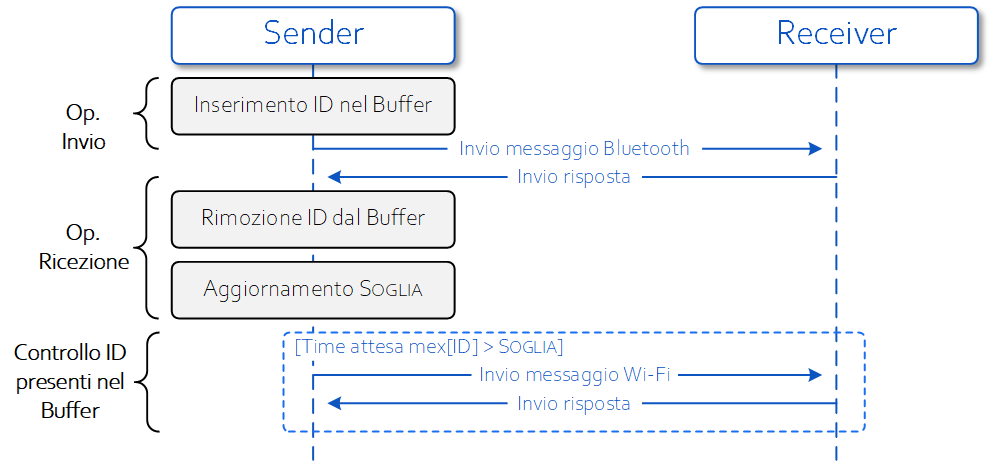
\includegraphics[width = \textwidth]{images/algoritmo_sequence.png}
    \caption{Sequence Diagram - Algoritmo Dinamico}
    \label{fig:sequence_algorithm}
\end{figure}

\noindent Osservando la figura \ref{fig:sequence_algorithm} relativa al comportamento dell'algoritmo dinamico è possibile individuare un'operazione d'invio che prevede appunto l'invio di un messaggio tramite la tecnologia Bluetooth, dopo avere memorizzato l'identificativo corrispondente all'interno di un Buffer. Questa operazione verrà eseguita con una frequenza definita in base al testbed da eseguire. \\
In seguito, qualora il messaggio non risulterà perso, si verificherà un'operazione di ricezione, la quale verrà innescata, dal ricevimento di una risposta. A seguito seguiranno le operazioni che consentiranno la rimozione dell'identificativo corrispondente dal Buffer e l'aggiornamento del valore di soglia.\\
Con la medesima frequenza con cui viene effettuata l'operazione d'invio, verrà eseguita anche l'operazione di check degli identificativi presenti all'interno del Buffer. Qualora il tempo d'attesa di un identificativo risulterà maggiore del valore di soglia, allora si procederà con l'invio impiegando la tecnologia Wi-Fi.\\

\noindent Una volta implementato il codice che consentirà di operare come preannunciato si passerà alla fase di valutazione del modello realizzato. La valutazione in merito al comportamento della rete riguarderà sia il variare della distanza tra mittente e destinatario sia il variare del carico di lavoro. Con `carico di lavoro', si intende la frequenza con cui vengono immessi i messaggi nella rete e ai fini della valutazione è molto importante il metodo di comunicazione request-response. Utilizzando tale paradigma, un messaggio viene definito come perso, solo nel momento in cui non sopraggiunge al Client la risposta da parte del Server.

%%%%% L'obiettivo principale prevede l'utilizzo della tecnologia BLE poiché comporta meno dispendio d'energia in trasmissione e nel momento in cui la rete risulta essere piuttosto carica di lavoro si potrebbe verificare la perdita di alcuni pacchetti durante la comunicazione. L'algoritmo realizzato consente di stabilire, in tempo reale, quando un pacchetto risulta perso e solo in tale circostanza inviarlo tramite la tecnologia di supporto. Con tale algoritmo si è cercato di evitare duplici invii e quindi giudicare troppo frettolosamente lo stato di un pacchetto e allo stesso tempo minimizzare il più possibile i ritardi relativi alla ritrasmissione di un pacchetto giudicato perso. La soglia che consente di definire come ``perso'' un pacchetto risulta essere dinamica, varia in base alla condizioni della rete.

\begin{figure}[!ht]
    \centering
    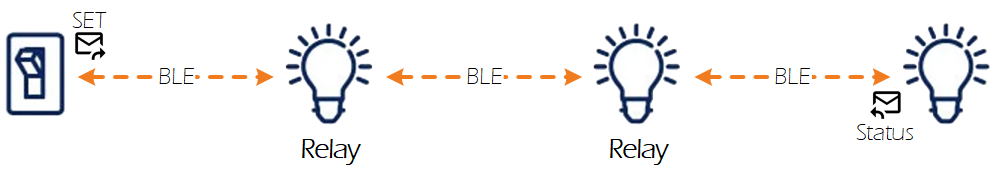
\includegraphics[width = \textwidth]{images/Mesh_network_2.png}
    \caption{rete Bluetooth Mesh}
    \label{fig:mesh_network}
\end{figure}

\noindent Come descritto nella sezione \textit{\nameref{subsub:messaggi}} (\ref{subsub:messaggi}), la comunicazione tra i nodi della rete può avvenire tramite diverse tipologie di messaggi. Tra le tipologie supportate si è pensato di impiegare messaggi di tipo \texttt{SET}, in grado non solo di modificare lo stato di un elemento e quindi rendere percepibile all'utente la ricezione e la gestione di un messaggio, ma anche in grado supportare il meccanismo di acknowledgment e quindi garantire un feedback anche al dispositivo mittente. Quindi alla ricezione di un messaggio ad esso destinato, il nodo provvederà ad attuare il cambio di stato comunicato e successivamente procederà all'invio di un feedback (conferma di ricezione) al mittente. Per quest'ultimo messaggio, lo standard prevede una tipologia appropriata, ovvero un messaggio di tipo \texttt{STATUS}, il quale contiene lo stato assunto dall'elemento interessato.\\

\noindent Con l'impiego di questa modalità di comunicazione, garantita direttamente dallo standard Bluetooth Mesh, si riesce a soddisfare il criterio di comunicazione bidirezionale, ma analizzando ulteriormente le specifiche definite dallo standard in termini di gestione dei messaggi ci ha portato a supporre l'eventualità del sorgere di alcune problematiche legate alla modalità di comunicazione che avremmo voluto ottenere. \\ % Invio di un mex alla stessa destinazione solo dopo aver atteso la scadenza del timer o la ricezione del ack 
La tipologia di messaggi (con acknowledgment) prevede la configurazione di un parametro ``timeout'' al fine di determinare l'evento di perdita e procedere con una ritrasmissione del messaggio. Questo stratagemma, fornito direttamente dallo standard, fa sì che finché non viene innescato tale evento o non viene ricevuta la conferma di ricezione, il sistema impedisce l'invio di ulteriori messaggi alla medesima destinazione. Solo al verificarsi di una delle due condizioni è possibile inviare un nuovo messaggio a tale indirizzo. \\
Ai fini di questo lavoro la suddetta situazione risulta essere troppo stringente, allora si è provveduto ad implementare un meccanismo specifico evitando di utilizzare il meccanismo di acknowledgment fornito dallo standard.\\ 
Il meccanismo proposto prevede lato mittente l'utilizzo di semplici messaggi sempre di tipo \texttt{SET}, ma questa volta senza acknowledgment. L'impiego di un messaggio di tipo \texttt{SET} consente di innescare un cambiamento di stato nel dispositivo destinatario, il quale invece, dovrà supportare un meccanismo di risposta personalizzato al fine di garantire l'avvenuta ricezione di un determinato messaggio. Il destinatario, alla ricezione di un determinato messaggio, dovrà elaborarlo e individuare l'elemento e lo stato da attuare, dopodiché procedere con la creazione di un messaggio di risposta (di tipo \texttt{STATUS}) contenente lo stato assunto. Dopo aver eseguito tutte queste operazioni potrà spedire il messaggio al client e procedere con l'attuazione del cambiamento di stato comunicato.\\ % Failed to send Generic Set message --- Busy sending message to DST

\noindent Per costruire una rete così come mostrato in figura \ref{fig:mesh_network} è necessario introdurre dei dispositivi intermedi al fine di garantire, al messaggio, il raggiungimento del destinatario. Tali dispositivi avranno il compito di inoltrare all'interno della rete tutti quei messaggi non destinati ad essi, rispettando le specifiche relative alla feature ``relay'' messa a disposizione da Bluetooth Mesh (\textit{\nameref{subsub:features}}) ed eseguendo il meccanismo di flooding dei dati descritto nella sezione \textit{\nameref{subsub:managed_flooding}}. Una volta implementata tale rete, nel rispetto delle specifiche descritte in precedenza,
si procederà alla valutazione delle prestazioni eseguendo dei testbed. La predetta configurazione prevederà esclusivamente l'impiego della sola tecnologia Bluetooth Mesh.\\
Poiché l'impiego di questa tecnologia risulta molto soggetta alle interferenze e alle condizioni dell'ambiente circostante si è pensato ad una riduzione sostanziale delle prestazioni nel momento in cui il carico di lavoro risulterà oneroso, con conseguenza congestione della rete, la quale comporterà una perdita di pacchetti ed un aumento della latenza.\\
Per fronteggiare una tale situazione e quindi garantire delle prestazioni elevate della rete anche con un carico di lavoro oneroso si è pensato di accostare un'altra tecnologia, al fine di ripartire il lavoro tra le due tecnologie, portando ad avere ottime prestazioni in qualsiasi circostanza. La scelta della tecnologia di supporto è ricaduta su \texttt{IEEE 802.11}, poiché ampiamente presente in qualsiasi tipologia di apparato di quotidiano utilizzo.\\
Inizialmente, si è pensato di adottare l'approccio Wi-Fi Mesh, in modo da avere la medesima infrastruttura di rete per entrambe le tecnologie. Con la possibilità di interconnettere i nodi, distribuiti su una vasta area fisica, sotto un'unica WLAN (Wireless Local-Area Network), in cui non si ha un singolo nodo centrale, denominato Acess Point, direttamente collegato a tutti gli altri nodi, bensì ai singoli nodi è consentito connettersi con i nodi vicini, i quali si assumono la responsabilità reciproca di divulgare la comunicazione all'interno della rete.\\
A seguito di opportune osservazioni è stato individuato, che adoperare sul medesimo nodo sia la tecnologia Bluetooth Mesh sia la tecnologia Wi-Fi Mesh risultava infattibile per la quantità di memoria richiesta per il loro funzionamento. Difatti, il modus operandi legato a tali tecniche prevede una quantità di memoria nettamente maggiore di quella di cui risultano dotati dei semplici dispositivi a nostra disposizione (\texttt{ESP32}). \\
Analizzando anche l'area di copertura dei dispositivi, in cui il raggio di trasmissione garantito dalla tecnologia Bluetooth è nettamente inferiore rispetto a quello Wi-Fi, ci è sembrato alquanto oneroso e poco produttivo l'impiego di un tale approccio, poiché tale area sarebbe stata coperta anche impiegando una rete Wi-Fi tradizionale.\\
Quindi, per la tecnologia di supporto si è ricorso all'utilizzo di una rete Wi-Fi tradizionale, la quale ci avrebbe garantito la possibilità di comunicare con tutti gli apparati che andranno a costituire la rete in un contesto indoor e non avremmo avuto problemi, in termini di memoria, in fase d'esecuzione. Tale approccio prevederà l'introduzione di un'entità esterna avente la funzione di Access Point (\texttt{AP}) a cui saranno direttamente connessi tutti gli altri nodi della rete e a cui spetterà il compito di inoltrare il pacchetto al nodo destinatario.

\begin{figure}[!ht]
    \centering
    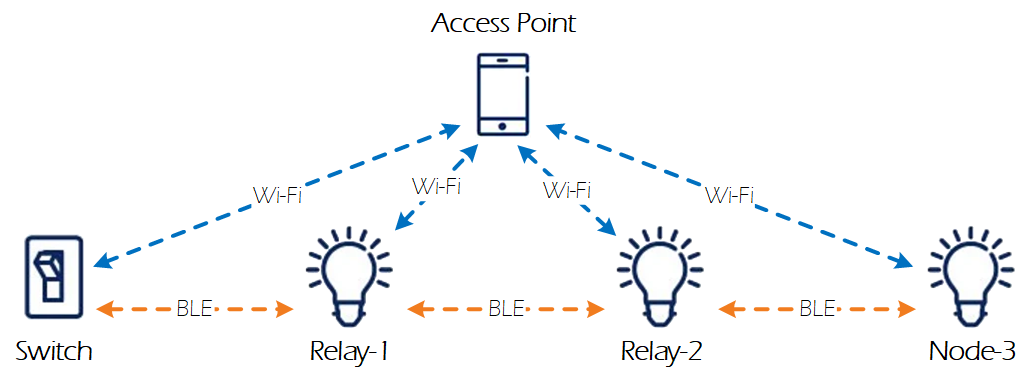
\includegraphics[width = \textwidth]{images/BLE_WiFi_2.png}
    \caption{rete Bluetooth Mesh - Wi-Fi}
    \label{fig:mesh_network_wifi}
\end{figure}

% La suddetta tecnologia, però, prevede un dispendio d'energia maggiore per la trasmissione di un pacchetto e in base a ciò si è presupposto che il raggio di copertura garantito da quest'ultima risultasse nettamente maggiore rispetto a quello del BLE, quindi impiegando un solo access point si potrà comunque garantire la comunicazione tra tutti gli apparati che andranno a costituire la rete in un contesto indoor.

\noindent Definite le tecnologie da impiegare nel seguente lavoro è stato necessario determinare come farle interagire tra loro al fine di diminuire la perdita di pacchetti, minimizzare i ritardi in fase di ritrasmissione e cercare di salvaguardare i consumi energetici.\\
Per fronteggiare tale situazione si è pensato di utilizzare come tecnologia preferita, lo standard Bluetooth Mesh e nel momento in cui si identifica la perdita di un pacchetto provvedere alla ritrasmissione utilizzando la tecnologia di supporto (più dispendiosa dal punto di vista energetico). In tal modo, con l'alternanza delle due tecnologie si allevia il carico di lavoro sulla tecnologia principale e allo stesso tempo si cerca di mantenere alte le performance delle rete.\\

\noindent Osservando la figura \ref{fig:sequence_algorithm_2} possiamo individuare le due fasi che costituiscono l'algoritmo descritto in precedenza. Tale algoritmo, inizialmente si troverà in uno stato di sleep, nel quale sarà possibile inviare solo messaggi attraverso la tecnologia Bluetooth, il che consentirà alla rete di giungere a pieno regime. Una volta giunto in tale stato si passerà ad una modalità attiva in cui si procederà sempre all'invio dei messaggi impiegando un tasso trasmissivo determinato dal testbed da eseguire. Nel mentre si eseguirà l'operazione di invio tramite Bluetooth, verrà analizzato lo stato della rete e ogni qualvolta verrà innescato l'evento di ricezione si procederà con l'operazione di ricezione (mostrata nel grafico \ref{fig:sequence_algorithm}) che comprenderà anche l'aggiornamento della soglia. Contemporaneamente, verrà eseguito anche il controllo sugli identificativi per verificare se ci sono pacchetti definiti ``persi''. Nel caso l'esito di tale controllo risulterà positivo, allora si procederà con l'invio del pacchetto tramite il Wi-Fi.

\begin{figure}[!ht]
    \centering
    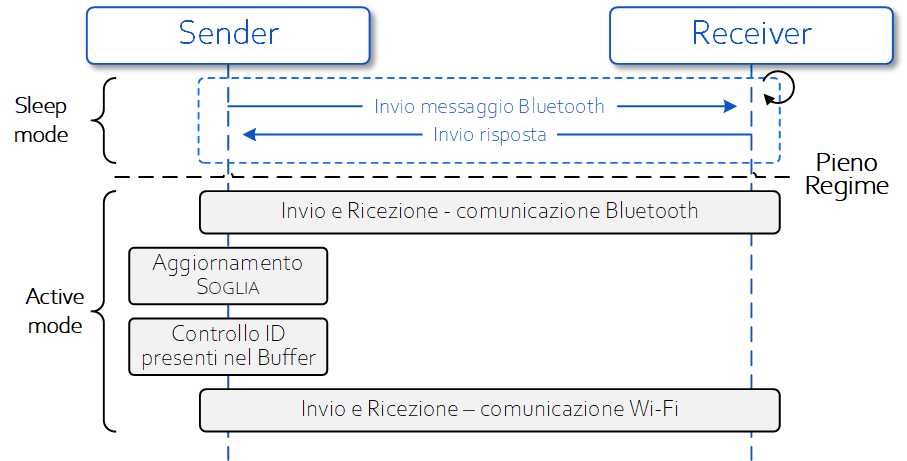
\includegraphics[width = 0.99\textwidth]{images/algoritmo_sequence_2.png}
    \caption{Sequence Diagram - Algoritmo Dinamico}
    \label{fig:sequence_algorithm_2}
\end{figure}

\noindent La realizzazione di una tale soluzione è stata pensata avvalendosi di un buffer contenente l'identificativo del messaggio da inviare. All'atto dell'invio di un messaggio tramite Bluetooth, l'identificativo corrispondente verrà inserito nel buffer e verrà rimosso solo nel momento in cui avverrà la ricezione del corrispondente messaggio di risposta, altrimenti, trascorso un intervallo di tempo, definito dal valore di soglia, verrà trasmesso un nuovo messaggio contenente il medesimo identificativo, questa volta però, utilizzando la tecnologia Wi-Fi (soluzione mostrata in figura \ref{fig:sequence_algorithm}. 
Operando in questo modo si tenterà di decongestionare la trasmissione Bluetooth, utilizzata per la gestione di gran parte dei messaggi.  

\begin{figure}[!ht]
    \centering
    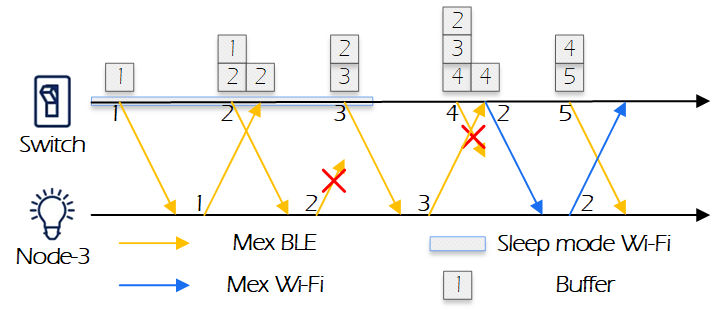
\includegraphics[width = \textwidth]{images/Algoritmo_dinamico.png}
    \caption{Algoritmo dinamico per utilizzare la tecnologia BLE Mesh e Wi-Fi}
    \label{fig:algoritmo dinamico}
\end{figure}

\noindent Così come accaduto con la prima soluzione, anche quest'ultima dovrà essere valutata. Quindi, implementati tutti i nodi, affinché si potessero usare entrambe le tecnologie, si è passati alla definizione dei casi di test.\\
L'idea a monte è quella di definire un intervallo di tempo, ovvero la durata del test e andare a modificare la frequenza con cui i messaggi vengono immessi nella rete, in modo da comprendere il suo comportamento nelle varie situazioni. 
Un'altra idea prevede di variare la distanza tra il nodo mittente e il destinatario e allo stesso tempo l'introduzione di nodi intermedi, facendo sì che ogni messaggio inviato passasse attraverso tali nodi prima di giungere a destinazione.\\
Una volta stabiliti i test è sorto il dilemma di come comunicare il test da eseguire. Ovvero come configurare un nodo affinché venisse eseguito un determinato test, anche perché le configurazione e i parametri risultavano essere diversi.\\
Una soluzione molto semplice, ma piuttosto dispendiosa, sarebbe stata quella di modificare i parametri del test direttamente mettendo mano all'interno dal codice. Lo svantaggio di tale soluzione riguardava il tempo impiegato, ogni qualvolta si cambiasse test, per modificare i parametri e successivamente reinstallare il codice sulla board. Per evitare tutte queste operazioni, si è pensato ad una soluzione un po' più complessa da gestire inizialmente, che però una volta definita, consentisse di comunicare qualsiasi configurazione al nodo senza dover caricare ogni volta il codice sulla board. Anche se tale processo coinvolgerà solo il nodo avente l'incarico di immettere i messaggi nella rete.\\
Così facendo il nodo potrà ricevere la configurazione e comportarsi di conseguenza. La soluzione prevede l'impiego di una comunicazione seriale, attraverso la quale sarà possibile indicare mediante una regola i parametri necessari al fine di configurare il nodo, avviare la simulazione ed ottenere in output il log di tale test.\\
L'operazione di configurazione riguarderà un solo nodo all'interno della rete, identificato con il nome di client, il quale avrà l'incarico di immettere i messaggi per gestire i vari elementi di cui essa risulta essere composta. Tale nodo può essere visto come un telecomando in grado di gestire l'accensione e lo spegnimento ma, anche la gestione della luminosità di un qualunque altro dispositivo inglobato nella rete, come potrebbero esserlo delle luci presenti all'interno di un contesto abitativo.\\
Cercando la soluzione efficace per affrontare questa problematica emersa, si è pensato all'impiego di un dispositivo \texttt{UART}\footnote{\textit{Universal Asynchronous Receiver-Transmitter}, un dispositivo hardware utilizzato per far dialogare tramite porta seriale un dispositivo di input/output con il nodo client}.

\begin{figure}[!ht]
    \centering
    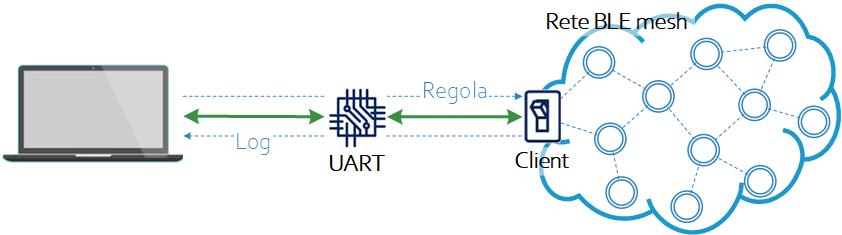
\includegraphics[width = \textwidth]{images/Uart.png}
    \caption{Architettura Rete BLE mesh - Test}
    \label{fig:mesh_network_uart}
\end{figure}

\noindent L'impiego di semplici dispositivi dotati di non molta memoria (tra l'altro sfruttata al massimo per poter eseguire i due stack protocollari) ha fatto sì che la creazione di un file di log, necessario per poter eseguire future analisi sull'operato, avvenisse non sul nodo ma su un dispositivo esterno. Anche in tale circostanza ci è venuto in soccorso il dispositivo \texttt{UART}. Poiché esso consente una comunicazione bidirezionale, potrà essere sfruttato anche per comunicare il verificarsi di ogni singolo evento di nostro interesse.\\

\noindent Per poter passare all'esecuzione dei testbed e vedere all'opera quanto è stato realizzato è fondamentale, come previsto dallo standard, un processo di provisioning al fine di consentire la creazione della nostra rete. In base a quanto detto nel capitolo \ref{ch:Ble_mesh}, il procedimento di provisioning prevede l'impiego di un dispositivo avente il ruolo di provisioner (sezione \ref{sec:provisioning}).
A tal proposito verrà adoperando uno smartphone con su installata un'apposita applicazione che consentirà la creazione, la configurazione e la gestione della rete mesh. Una volta creata la rete e configurati tutti i nodi sarà possibile procedere con l'esecuzione dei test utilizzando i parametri di configurazione ricevuti appositamente tramite seriale.\\
Con l'impiego di entrambe le tecnologie, il dispositivo una volta entrato a far parte della rete mesh non avrà concluso la fase di configurazione, ma dovrà procedere con la sottoscrizione ad una determinata rete Wi-Fi, utilizzata solo per trasmettere i messaggi (denominati come `persi' con la tecnologia BLE mesh) tra i nodi della rete. \\
Solo dopo aver inizializzato e configurato entrambe le tecnologie, la fase di configurazione risulterà terminata e sarà possibile procedere con la fase di test vera e propria.\\

\noindent Gli eventi generati durante l'esecuzione del test verranno memorizzati attraverso un file di log e in secondo luogo, verranno analizzati ed infine confrontati i risultati ottenuti dall'esecuzione delle due soluzioni descritte in questo capitolo.\\

    \chapter{Implementazione}
\label{ch:implementazione}

In questa sezione verranno descritte le scelte implementative ed i componenti impiegati che hanno consentito la realizzazione di una rete in rispetto delle specifiche definite nel capitolo di \textit{\nameref{ch:progettazione}}.\\ 
Il seguente lavoro di tesi ha previsto la definizione di due approcci così strutturati: nel primo si è utilizzata solo la tecnologia \texttt{Bluetooth Mesh}, mentre nel secondo è stata integrato lo standard \texttt{802.11} come tecnologia di supporto.\\
In entrambi gli approcci sono stati utilizzati quattro dispositivi ESP32 con i seguenti ruoli: 

\begin{itemize}
    \item un dispositivo \textit{client} il cui compito è quello di inviare i messaggi all'interno della rete con una frequenza indicata in input dall'utente, avvalendosi di uno script \texttt{Python}. In più, è in continua comunicazione, tramite porta seriale, con il PC per assicurare la definizione di un file di log. 
    
    \item due dispositivi aventi il ruolo di \textit{relay}. Sfruttati solo con la tecnologia Bluetooth Mesh, poiché con la tecnologia 802.11 è stato necessario introdurre un dispositivo esterno, con il ruolo di \textit{router}.
    
    \item un dispositivo \textit{server} avente il compito di ricevere dei messaggi precedentemente inviati dal client, attuare il cambiando di stato comunicato e confermare tale ricezione utilizzando la medesima tecnologia del messaggio ricevuto.
\end{itemize}

\noindent Per garantire la creazione della rete mesh è stato necessario l'utilizzo di un dispositivo in grado sia di supportare un'applicazione di provisioning sia in grado di eseguire le operazioni di routing per la tecnologia Wi-Fi. Per soddisfare entrambe queste richieste è stato adottato uno smartphone con supporto a Bluetooth 5. Oltre a tale dispositivo è stato necessario l'impiego di un PC non solo per programmare i vari nodi attraverso il framework \texttt{ESP-IDF} ma anche per consentire la comunicazione con il nodo client, necessaria per comunicare il comportamento da assumere e per ricevere e archiviare gli eventi innescati su tale nodo durante l'esecuzione del test.

\section{Dispositivi}
Come anticipato all'inizio del capitolo, per la realizzazione del seguente progetto di tesi sono stati coinvolti i seguenti dispositivi. Di seguito una breve descrizione.
\subsection{ESP32}
% http://esp32.net/
% https://en.wikipedia.org/wiki/ESP32
% https://www.espressif.com/en/products/hardware/esp32/overview
% http://www.lucadentella.it/2016/12/03/esp32-1-introduzione/
% https://www.zerozone.it/tecnologia-privacy-e-sicurezza/primi-esperimenti-di-iot-con-i-moduli-esp32/13230
Il dispositivo ESP32 indica una serie di microcontrollori a basso costo e a bassa potenza il cui chip è in grado di supportare le tecnologie di comunicazione \texttt{Wi-Fi} e \texttt{dual-mode Bluetooth}. \\
A settembre 2016 Espressif Systems (una società cinese con sede a Shangai) ha annunciato e reso disponibile il chip successore ad ESP8266, chiamato appunto ESP32, il quale ha introdotto un numero maggiore di pin GPIO, la presenza della connettività Bluetooth, un sensore touch e maggiore memoria.\\ 
Il nucleo di questi nuovi dispositivi è costituito da un microprocessore Tensilica Xtensa LX6 a 32-bit nelle varianti single-core o dual-core, in grado di operare con una frequenza comprese tra 80 e 240 MHz.\\
L'integrazione di Bluetooth, Bluetooth Low Energy e Wi-Fi garantiscono  l'impiego in una vasta gamma di scenari sopratutto in contesti IoT. Il Wi-Fi garantisce la copertura di una zona piuttosto ampia ed una diretta connessione ad Internet tramite l'utilizzo di un router Wi-Fi, mentre il Bluetooth consente lo scambio di informazioni su un'area nettamente inferiore ma con consumi nettamente più bassi. 
Il ridotto consumo energetico è garantito grazie a specifiche funzioni, tra cui la gestione dei clock e il ridimensionamento dinamico della potenza.\\

\noindent Una scheda di sviluppo dotata di chip ESP32, per poter funzionare necessita di alcuni componenti esterni a tale chip: una memoria flash (in cui sono memorizzati il firmware e i dati), un modulo per il Real Time Clock (RTC), un'antenna e alcuni componenti passivi.\\
Sul mercato, si trovano diverse tipologie di circuiti stampati personalizzati con su integrato il chip ESP32. Oltre al chip tale board sono dotate di appositi moduli tra l'altro estendibili, grazie al numero elevato di PIN I/O i quali consentono di sviluppare progetti sempre più complessi.\\
Tali schede montano uno stabilizzatore di tensione che permette la corretta alimentazione dei moduli, il convertitore \texttt{USB-UART} e i tasti \texttt{RESET} e \texttt{FLASH} che semplificano il processo di programmazione. \\
Esistono diversi firmware per gestire questi chip, quello utilizzato in tale circostanza risulta essere il firmware ufficiale, ovvero quello rilasciato da \texttt{Espressif} e consente la comunicazione con il modulo attraverso dei comandi AT. % comandi AT -> particolari stringhe utilizzare per comunicare con diversi dispositivi elettronici.
Un firmware alternativo, di tutto rilievo, è chiamato NodeMCU ed è basato su Lua, un linguaggio di programmazione dinamico e veloce simile al Python.\\

\noindent In base alle necessità richieste dal seguente progetto, ovvero poter utilizzare contemporaneamente lo stack Wi-Fi e BLE, sono stati utilizzati dispositivi \textit{ESP32-WROVER} dotati di una memoria supplementare rispetto ai dispositivi \textit{ESP32-WROOM} maggiormente diffusi.\\
Nello specifico ESP32-WROVER presenta una memoria Flash SPI di 4 MB ed una Pseudo Static RAM (PSRAM) aggiuntiva di 8 MB.
\begin{figure}[!ht]
    \centering
    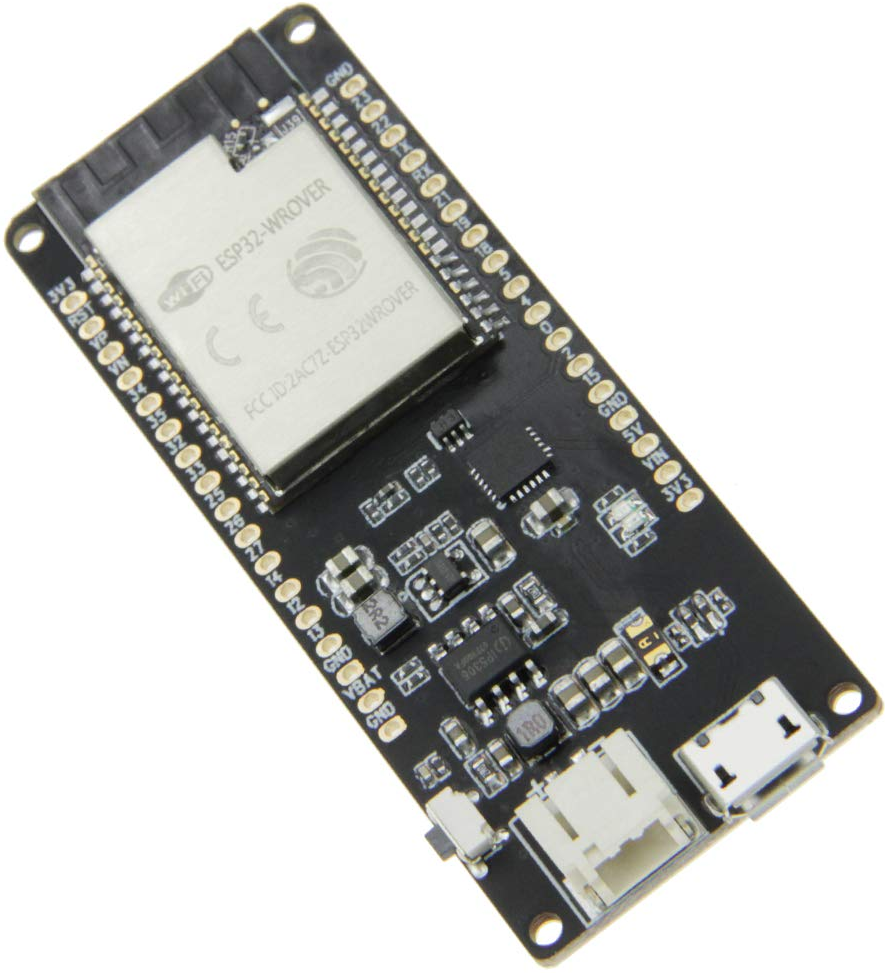
\includegraphics[width = 0.5\textwidth]{images/esp32_wrover.png}
    \caption{ESP32 WROVER}
    \label{fig:esp32_wrover}
\end{figure}

\subsubsection{Ambiente di sviluppo}
Per sviluppare un applicativo eseguibile su tali dispositivi la scelta può ricadere su diversi ambienti di sviluppo. Di seguito una rapida descrizione di \texttt{Arduino IDE}, molto semplice da utilizzare, e il framework messo a disposizione da Espressif (\texttt{ESP-IDF}) utilizzato in questo contesto applicativo.\\
Arduino IDE è un framework open-source che consente di avere un approccio piuttosto semplice per la programmazione dei moduli e per l'upload del codice sulle board compatibili con l'IDE. Prima di procedere con la compilazione del codice da copiare sulla propria board, è fondamentale aggiungere le apposite librerie al fine di rendere la board compatibile, nel caso in cui non lo era.\\
% http://wiring.org.co/
Utilizzando Arduino IDE è possibile creare un applicativo (sketch) per il proprio microcontrollore sfruttando una libreria software del progetto \textit{Wiring}. Wiring oltre ad essere una piattaforma di prototipazione open-source, fornisce delle regole per la strutturazione del codice relativo alle comuni procedure di input e di output utilizzando un linguaggio di programmazione derivato dal \texttt{C++}.\\
% https://en.wikipedia.org/wiki/Arduino_IDE
Il codice scritto dall'utente richiede solo due funzioni base: 
\begin{itemize}
    \item \textit{setup}: una funzione eseguita solo una volta, all'avvio dello sketch e può essere usata per definire le impostazioni iniziali dell'ambiente.
    \item \textit{loop}: una funzione invocata continuamente, finché la board non viene spenta. Tale funzione descrive il comportamento che dovrà assumere il dispositivo durante il suo periodo di attività.
\end{itemize}
Una volta creato lo sketch e configurato l'IDE per supportare la board in possesso è possibile procedere con l'upload del codice e interagire (attraverso la seriale) con l'applicativo grazie agli strumenti messi a disposizione da Arduino IDE.\\

% http://www.lucadentella.it/2016/12/12/esp32-2-lambiente-di-sviluppo/
% https://github.com/espressif/esp-idf
\noindent L'alternativa ad Arduino IDE per programmare i chip in dotazione è Espressif IoT Development Framework (ESP-IDF), rilasciata proprio dalla casa produttrice e indicata come il framework ufficiale di prototipazione per tali board.
Come il tool precedente, anche esso risulta essere open-source e cross-platform (disponibile per Windows, Linux e Mac OS), anche se il suo utilizzo è sensibilmente più complicato e qualsiasi operazione deve essere svolta tramite console.\\
Il framework ESP-IDF è reperibile presso il repository ufficiale \href{https://github.com/espressif/esp-idf}{GitHub} di Espressif: \url{https://github.com/espressif/esp-idf}. Dopo aver scaricato, installato e configurato l'intero ambiente (variabili d'ambiente, toolchain per compilare il codice, tools per la creazione di un'applicazione) e possibile finalmente implementare un'applicazione eseguibile da un dispositivo Espressif.\\
Come indicato dalla documentazione ufficiale, le operazione relative ad ogni progetto da eseguire sui predetti dispositivi sono indicate in seguito e prevedono sempre l'utilizzo dell'istruzione \texttt{idf.py}. Le seguenti istruzioni dovranno essere eseguite solo dopo essersi posizionati nella directory del progetto da gestire.
\renewcommand{\theenumi}{\roman{enumi}}
\begin{enumerate}
    \item \texttt{idf.py menuconfig}: consente la configurazione del progetto in base al dispositivo che dovrà eseguirlo. Con il seguente comando si ottiene un menu che consente di specificare determinati parametri riguardanti ``\texttt{SDK tool configuration}'', ``\texttt{Bootloader config}'', ``\texttt{Serial flasher config}'', ``\texttt{Partition Table}'', per citarne alcuni. \\
    All'interno di tale menu, oltre alle voci menzionate, è possibile definire una voce ``\texttt{Example Configuration}'' che, attraverso un'estensione basata su Python (kconfiglib), fornisce un meccanismo di configurazione del progetto in fase di compilazione. Il file \texttt{kconfig} consente all'utente di specificare apposite informazioni in base al dispositivo in uso. Ad esempio, tramite questo file è possibile indicare l'\textit{SSID} della rete Wi-Fi a cui il dispositivo dovrà connettersi e la rispettiva \textit{password}.
    
    \item \texttt{idf.py build}: consente la compilazione dell'intero progetto (app, bootloader e partition table) in base ai parametri di configurazione. 
    
    \item \texttt{idf.py -p PORT flash}: consente di copiare l'intero progetto sul dispositivo connesso tramite la porta specificata nel comando (\texttt{PORT} deve essere rimpiazzato con il nome della porta seriale di riferimento e varia in base al sistema operativo in uso, ad esempio in Windows con \texttt{COM1}, su Linux con \texttt{/dev/ttyUSB0} e su MacOS con \texttt{/dev/cu.usbserial-X}).
    
    \item \texttt{idf.py -p PORT monitor}: consente di visualizzare l'output fornito dal dispositivo ESP32 sulla porta seriale che lo connette al PC (\texttt{PORT} rimpiazzato sempre con la corrispondente porta seriale).
\end{enumerate}

\noindent I comandi elencati rappresentano solo un minima parte tra tutti quelli possibili. Per accedere all'intera lista di istruzioni che consentono la configurazione di un'applicazione è possibile utilizzare il comando \texttt{idf.py ---help}. Tramite l'istruzione \texttt{--help} è possibile individuare anche le opzioni relative ad uno specifico comando (\texttt{idf.py <command> ---help}, ad esempio \texttt{idf.py monitor ---help}). In più è concesso anche combinare più comandi in una sola istruzione (\texttt{idf.py -p PORT clean flash monitor}).\\
Nel caso in cui è stata eseguita una modifica ai parametri di configurazione, è possibile eseguire direttamente l'istruzione \texttt{idf.py flash} che si occuperà per prima cosa di compilare il progetto qualora un file sorgente risultasse modificato ed in seguito provvederà a fare l'upload sul dispositivo connesso tramite la porta seriale specificata.\\

\noindent Il seguente ambiente di sviluppo fornisce degli esempi da cui partire per la creazione di un applicativo che utilizza le tecnologie supportate. Partendo dall'esempio messo a disposizione in merito a Bluetooth Mesh è iniziato a prender vita il seguente progetto di tesi. \\
L'esempio comprende l'implementazione di due tipi di nodi, client e server, configurati secondo il modello \texttt{Generic OnOff Model}. Tali esempi per essere funzionanti prevedono l'impiego di un \texttt{Configuration Server Model} per la configurazione della rete e del codice per gestire il processo di provisioning.

% http://www.lucadentella.it/2016/12/22/esp32-4-flash-bootloader-e-freertos/
\subsubsection{Memoria} 
Il chip ESP32 richiede una memoria flash esterna nella quale memorizzare l'applicativo, i dati, i parametri di configurazione, etc. Essa risulta essere collegata al chip attraverso un bus SPI e può avere una dimensione massima di 16 MB. Tale memoria risulta essere divisa in partizioni e l'elenco delle diverse partizioni, della loro dimensione e della loro posizione è memorizzato nella flash stessa (all'indirizzo 0x8000). Dal menu \texttt{Partition Table} è possibile decidere come organizzare tale memoria in base alle proprie esigenze, specificando il nome del file \texttt{CSV} che contiene una versione personalizzata oppure utilizzare una delle due configurazioni predefinite fornite da Espressif.\\
Con il seguente lavoro, per adoperare i due stack protocollari sul medesimo nodo è stato necessario caricare una tabella delle partizioni personalizzata.

\subsubsection{FreeRTOS}
% https://exploreembedded.com/wiki/Hello_World_with_ESP32_Explained
% https://freertos.org/
% https://aws.amazon.com/it/freertos/
Il framework \texttt{ESP-IDF} utilizza un sistema operativo definito appositamente per microcontrollori, Real-Time Operating System (FreeRTOS), in grado di sfruttare al meglio i due processori e gestire le numerose periferiche integrate di un ESP32. Distribuito gratuitamente con licenza open-source, FreeRTOS include un kernel in grado di svolgere operazioni semplici e funzionali eseguibile su dispositivi a basso consumo ed offre un insieme sempre crescente di librerie adatte in molteplici contesti industriali e per svariate applicazioni. Questo sistema operativo è sviluppato dando una particolare enfasi all'affidabilità e alla facilità di utilizzo.\\
Non bisogna pensarlo come un sistema operativo di un PC, ma bensì un sistema operativo per sistemi embedded il cui compito è quello di offrire, tramite un proprio scheduler, il multitasking, ovvero la possibilità di pianificare ed eseguire più task contemporaneamente.
FreeRTOS offre un sistema real-time che consente la pianificazione dei task in modo deterministico, difatti consente al programmatore di definire la priorità dei propri task e lo scheduler utilizza proprio tali valori per definire la sequenza di esecuzione.\\
I vantaggi ed i motivi per cui viene utilizzato FreeRTOS in dispositivi con bassi consumi energetici sono i seguenti:
\begin{itemize}
    \item \textit{Open source}: FreeRTOS viene rilasciato con la licenza open-source MIT, una licenza permissiva che offre maggiori opportunità di riutilizzo del codice (progetti commerciali e personali).
    
    \item \textit{Kernel affidabile}: il kernel FreeRTOS è considerato dalle principali aziende a livello mondiale uno standard de facto per microcontrollori e microprocessori di piccole dimensioni grazie alla comprovata robustezza, impatto minimo in termini di memoria e il supporto di una vasta gamma di dispositivi.
    
    \item \textit{Semplicità e Rapidità di progettazione}: con demo preconfigurate e dettagliate integrazioni di riferimento in ambito IoT. Caratteristiche che consentono all'utente di realizzare in poco tempo un progetto e metterlo sul mercato.
    
    \item \textit{Flessibilità}: FreeRTOS offre la flessibilità per costruire facilmente soluzioni IoT su un'ampia gamma di chipset. Supporta oltre 40 tipologie di architetture.
    
    \item \textit{Sicurezza}: FreeRTOS include il supporto per il Transport Layer Security (TLS v1.2) al fine di favorire un collegamento sicuro ai dispositivi. Inoltre, è supportato l'aggiornamento sicuro (crittografato) over-the-air (OTA) per fornire ai dispositivi aggiornamenti (includono potenziamenti delle funzionalità o patch di sicurezza) anche dopo il loro rilascio con costi e sforzi minimi.
    
\end{itemize}

\subsection{nRF Mesh}
% https://www.nordicsemi.com/Software-and-tools/Development-Tools/nRF-Mesh
Un aspetto fondamentale per una rete mesh è proprio l'iter relativo alla sua creazione, ovvero il processo di provisioning (Sezione \ref{sec:provisioning}). In questa circostanza l'intero processo viene svolto adoperando uno smartphone con su installata un'apposita applicazione, disponibile sia per Android sia per iOS, in grado di semplificare determinate operazioni. L'applicazione in questione è nRF Mesh rilasciata dalla Nordic Semiconductor ASA con lo scopo di portare i naturali benefici dell'utilizzo di uno smartphone nelle attività di configurazione e controllo di una rete Bluetooth Mesh.\\

Come descritto nella sezione \ref{ch:Ble_mesh} lo standard Bluetooth Mesh opera al di sopra dello standard Bluetooth Low Energy e a tal proposito richiede ulteriori caratteristiche, tra cui quelle messe a disposizione dalla seguente applicazione, ovvero: 
\begin{itemize}
    \item \textit{Controllo di un nodo}: supporta la gestione di un modello GenericOnOff Server.
    \item \textit{Provisioning}: supporta l'autenticazione OOB di tipo numerico e l'autenticazione Static (ovvero senza interazione dell'utente) e si preoccupa di assegnare in modo automatico gli indirizzi unicast agli elementi di un nodo.
    \item \textit{Configurazione}: consente di impostare le chiavi di applicazione o generarle casualmente, creare indirizzi di tipo group e consentire la sottoscrizione dei nodi a tali indirizzi.
\end{itemize}
Inoltre, consente di eseguire appositi comandi di configurazione relativi alla rete mesh, tra cui definire un pubblication address per un modello, aggiungere o rimuovere la sottoscrizione di un elemento ad un determinato indirizzo, esplorare le caratteristiche di un nodo, etc..\\
L'aspetto rilevante e il motivo per cui è stata utilizzata nel seguente progetto riguarda le operazioni di provisioning e la possibilità di comunicare con qualsiasi tipo di dispositivo BLE in grado di supportare lo standard Bluetooth Mesh.

\subsection{Router Wi-Fi}
Al fine di consentire la comunicazione attraverso la tecnologia di supporto è stato necessario introdurre un dispositivo in grado di gestire il processo di instradamento dei pacchetti. A tal proposito è stato utilizzato uno smartphone sfruttando la funzionalità di ``\texttt{Router Wi-Fi}''. \\
Ai fini del progetto non è necessario che i dispositivi siano connessi ad Internet, difatti tale modalità viene utilizzata solo per consentire una comunicazione alternativa ai nodi della rete (figura \ref{fig:ruoli_rete_mesh}).

\section{Implementazione Nodi}
La realizzazione della rete mesh così come descritto nel capito di \nameref{ch:progettazione} (configurata come in figura \ref{fig:ruoli_rete_mesh}) ha previsto la definizioni di alcuni ruoli (Client e Server) essenziali per lo standard Bluetooth Mesh, il che ha comportato implementazioni leggermente differenti e l'impiego di due stack protocollari ben distinti.
Il ruolo di client è rilegato al dispositivo indicato come \texttt{Switch}, mentre il ruolo di Server è rilegato ai dispositivi \texttt{Relay-1}, \texttt{Relay-2}, \texttt{Node-3}.\\

\begin{figure}[!ht]
    \centering
    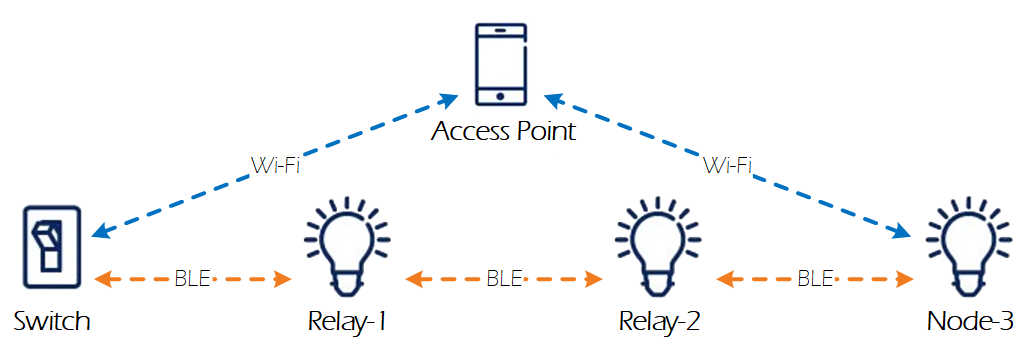
\includegraphics[width = \textwidth]{images/nodi_mesh.png}
    \caption{Ruoli rete Bluetooth mesh}
    \label{fig:ruoli_rete_mesh}
\end{figure}

\noindent Durante la fase di implementazione mi sono servito dell'ambiente di sviluppo \texttt{ESP-IDF}, poiché consente l'utilizzo di apposite librerie messa a disposizione da Espressif per la creazione di un applicativo utilizzando la tecnologia Bluetooth Mesh (la community di Espressif ha iniziato a lavorare al seguente standard solo a gennaio 2019). Al fine di evitare problematiche durante la fase implementativa in merito alle possibili modifiche giornaliere apportate dagli sviluppatori a tali librerie ho preferito focalizzare il lavoro utilizzando la versione \texttt{ESP-IDF v4.0-beta2}.\\ 

\noindent L'implementazione che consente ad un nodo di essere integrato all'interno di una rete mesh e quindi comprende l'intero processo di provisioning risulta essere identica per entrambe le tipologie di nodi (ereditata dall'esempio messo a disposizione da Espressif). Le due tipologie di ruoli, oltre a ciò, presentano un'altra caratteristica implementativa in comune, ovvero il numero di elementi di cui risultano composti. Ogni nodo è costituito da due elementi rappresentati tramite \texttt{LED} ed implementati per mezzo del modello \texttt{Generic Level Server Model}, il quale permette di comunicare l'intensità dell'illuminazione attraverso dei messaggi definiti dal \texttt{Generic Level Model}. A questi due \texttt{LED} viene aggiunto un terzo nel momento in cui viene utilizzata anche la tecnologia Wi-Fi.\\
I nodi \texttt{Relay-1}, \texttt{Relay-2} e \texttt{Node-3} presentano il medesimo codice, ad eccezion fatta per la feature \textit{relay}.\\

\noindent L'accensione di un ESP32 prevede una prima fase di inizializzazione del dispositivo a cui segue l'esecuzione dell'applicativo invocando il metodo \texttt{app\_main()}.\\
Poiché il chip ESP32 consente la memorizzazione di informazioni all'interno della memoria flash, per poter accedere a tali dati è necessario inizializzarla e per fare ciò viene utilizzata la funzione \texttt{nvs\_flash\_init()}.\\
Una volta inizializzata, si procede con l'inizializzazione degli stack da utilizzare nell'applicativo. Nel caso dell'approccio Bluetooth Mesh è necessario inizializzare per prima cosa lo stack Bluetooth Low Energy (\texttt{bluetooth\_init}) dopodiché procedere con l'inizializzazione dello standard Bluetooth Mesh (\texttt{ble\_mesh\_init}). Nel caso dell'approccio con entrambe le tecnologie, dopo avere eseguito le inizializzazioni appena descritte si procede con l'inizializzazione anche dello stack Wi-Fi.\\
Entrambi gli approcci oltre ad inizializzare gli stack relativi alle tecnologie di comunicazione da utilizzare, provvedono ad inizializzare anche dei \texttt{LED}. \\
Due \texttt{LED} utilizzati per rappresentare gli elementi di ciascun nodo e gestibili tramite lo standard Bluetooth ed un terzo \texttt{LED} gestito attraverso la tecnologia 802.11. L'impiego di tali \texttt{LED}, consente di identificare lo stato del dispositivo durante la fase di configurazione della rete Mesh ed il corretto funzionamento durante lo svolgimento della fase di test.\\
La conclusione della fase di inizializzazione viene segnalata all'utente con l'accensione di tutti i \texttt{LED} definiti per tale nodo.\\
Nel momento in cui il nodo presenta tutti i \texttt{LED} accessi allora sarà possibile procedere con il suo inserimento all'interno della rete Mesh. La definizione di tale rete avviene mediante l'applicazione \texttt{nRF Mesh}. Tale applicazione consente di individuare il dispositivo da integrare nella rete (scansionando l'ambiente circostante) e una volta individuato procedere al suo inserimento attraverso il processo di provisioning. La conclusione di tale processo viene segnalata con lo spegnimento dei \texttt{LED} associati alla tecnologia Bluetooth. Nel caso in cui l'approccio utilizzato prevede l'impiego della tecnologia Wi-Fi, al termine delle operazioni di provisioning BLE, il nodo procede automaticamente alla connessione con la rete Wi-Fi indicata (definita tramite \texttt{idf.py menuconfig}) e al termine di tale proceduta provvede a spegnere l'ultimo \texttt{LED} acceso.\\
Lo spegnimento di tutti i \texttt{LED} indica il corretto inserimento del nodo all'interno della rete e che è pronto per inviare o ricevere messaggi in base alla tecnologia supportata.\\

\noindent Durante la fase di configurazione dello stack BLE Mesh è prevista la registrazione di apposite funzioni di callback per notificare al livello applicativo il verificarsi di determinati eventi. Tali funzioni vengono innescate con la ricezione di un messaggio destinato ad uno degli elementi presenti nel nodo.\\
La ricezione e la gestione di un messaggio da parte di un elemento viene indicata all'utente cambiando lo stato del \texttt{LED} corrispondente (da \texttt{ON} ad \texttt{OFF} e viceversa). Poiché i \texttt{LED} sono l'unico strumento utilizzabile dai dispositivi per comunicare con l'utente, è stato preferito segnalare il verificarsi di questi eventi con il cambio di stato e non con variazioni graduali in base al valore contenuto nel messaggio ricevuto.

\subsection{Implementazione Client}
Il dispositivo Client, rappresentato nella figura \ref{fig:ruoli_rete_mesh} con il nome di ``\texttt{Switch}'' è quel dispositivo avente il compito di inviare i messaggi all'interno della rete mesh.\\
La natura dei messaggi è stata definita per mezzo del modello \texttt{Generic Level Model}, mentre la configurazione dell'ambiente di test (la tipologia, la frequenza d'invio, il nodo di destinazione) e quindi il comportamento del dispositivo viene comunicata per mezzo di porta seriale, avvalendosi del \texttt{USB-UART} e di uno script Python appositamente definito.\\
Poiché il seguente nodo risulta essere uno switch e quindi un interruttore generico per gestire il comportamento degli altri nodi della rete, è stato configurato utilizzando il modello \texttt{Generic Level Client Model}.
In questa sezione verrà mostrata l'implementazione del comportamento del nodo client distinguendo l'implementazione che ha permesso di definire il testbed per l'approccio Bluetooth Mesh e per l'approccio Bluetooth Mesh combinato con il Wi-Fi. Prima di descrivere i due approcci, verrà mostrato il codice appartenente al nodo Client che consente la comunicazione con il PC tramite seriale.\\

\noindent Dopo avere eseguito la configurazione delle tecnologie da utilizzare per la tipologia di approccio scelto, la prima operazione eseguita riguarda l'inizializzazione del \texttt{UART} e la definizione di un task specifico in grado di far dialogare i due dispositivi tramite porta seriale.\\

\noindent L'inizializzazione del \texttt{UART} avviene invocando la funzione \texttt{uart\_init} la quale prevede per prima cosa la configurazione del controller passando la struct \texttt{uart\_config\_t} (specificando la velocità di trasmissione, il numero di bit per ogni parola, l'utilizzo o meno di un bit di parità e la tipologia del controllo di flusso) come secondo parametro del metodo \texttt{uart\_param\_config} e come primo parametro il numero relativo al controller scelto. \\
Dopodiché si procede con la configurazione dei \texttt{PIN} ed infine si passa all'installazione del driver (\texttt{uart\_driver\_install}), andando a specificare oltre al numero del controller anche la dimensione dei buffer. L'inclusione del driver ``\texttt{driver/uart.h}'' consente di semplificare l'utilizzo di tale controller.\\

\begin{lstlisting}[language=C, caption= Configurazione e installazione driver \texttt{UART}]
void uart_init() {
    uart_config_t uart_config = {
            .baud_rate = 115200,
            .data_bits = UART_DATA_8_BITS,
            .parity = UART_PARITY_DISABLE,
            .stop_bits = UART_STOP_BITS_1,
            .flow_ctrl = UART_HW_FLOWCTRL_DISABLE
    };

    uart_param_config(UART_NUM_1, &uart_config);
    uart_set_pin(UART_NUM_1, TXD_PIN, RXD_PIN, UART_PIN_NO_CHANGE, UART_PIN_NO_CHANGE);
    uart_driver_install(UART_NUM_1, UART_BUF_SIZE * 2, 0, 0, NULL, 0);
}
\end{lstlisting}

\noindent L'utilizzo del \texttt{UART} avviene attraverso la definizione di un task (attività) specifico utilizzando il metodo \texttt{xTaskCreate}. Questo metodo richiede come parametri: il puntatore alla funzione che contiene il codice del task\footnote{I task devono essere implementati per non tornare mai}, il nome da assegnare al task (utile in fase di debugging), la dimensione dello stack di memoria (in words non in byte), i valori da passare come parametri alla funzione, la priorità con cui il task verrà eseguito e il puntatore (opzionale) per consentire la gestione del task tramite una funzione esterna. Una volta creato un task, lo scheduler di FreeRTOS lo manda in esecuzione in base alla priorità indicata.\\

\begin{lstlisting}[language=C, caption= Inizializzazione e definizione del task per utilizzare il \texttt{UART}]
void start_serial_communication(){
    uart_init();
    xTaskCreate(uart_task, "uart_task", 2048, NULL, 5, NULL);
}
\end{lstlisting}

\noindent La funzione (\texttt{uart\_task}) passata come parametro al metodo \texttt{xTaskCreate} contiene il codice che permette al nodo di essere in ascolto su una porta seriale e quindi poter ricevere un'istruzione. \\
Per acquisire i dati comunicati tramite porta seriale dal PC si utilizza l'istruzione \texttt{uart\_read\_bytes}. Una volta ricevuta la regola, il nodo procede, per prima cosa, a comprenderla (\texttt{count\_tokens}, \texttt{str\_split}) e successivamente ad attuarla adoperando la funzione \texttt{command\_received}.\\
\begin{lstlisting}[language=C, caption= acquisizione dati attraverso il \texttt{UART}]
static void uart_task(void *pvParameters) {
    uint8_t *data_uart = calloc(1, UART_BUF_SIZE);

    while (is_running_uart) {
        //Read data from the UART
        int rxBytes = uart_read_bytes(UART_NUM_1, data_uart, UART_BUF_SIZE, 100 / portTICK_RATE_MS);

        if (rxBytes > 0) {
            data_uart[rxBytes] = '\0';
            ESP_LOGI("UART", "Read %d bytes: '%s'", rxBytes, data_uart);

            char **tokens = str_split((char *) data, ',');
            command_received(tokens);

            fflush(stdout);
            uart_flush_input(UART_NUM_1);
        }
    }
    vTaskDelete(NULL);
}
\end{lstlisting}

\noindent La trasmissione di informazioni dal nodo Client al PC avviene per mezzo del dispositivo \texttt{UART} invocando l'istruzione \texttt{uart\_write\_bytes}. Tramite questa funzione si copia un array di caratteri nel buffer del driver e sarà quest'ultimo ad occuparsi, in modo autonomo, di gestire la comunicazione con il controller e l'effettivo invio dei dati. La funzione utilizzata prevede i seguenti parametri: il controller scelto, l'array di caratteri e la rispettiva dimensione. \\
La funzione riportata in seguito, \texttt{uart\_trasmitting}, prende in input un array di caratteri e dopo aver calcolato la dimensione procede a scrivere i dati nel buffer, così come descritto in precedenza.\\

\begin{lstlisting}[language=C, caption= operazione di trasmissione dati tramite lo strumento \texttt{UART}]
void uart_trasmitting(const char *event_s) {
    const int len = strlen(event_s);
    uart_write_bytes(UART_NUM_1, event_s, len);
}
\end{lstlisting}

\subsubsection{Istruzioni ed Eventi nodo Client}
\label{subsub:parametri_testbed}
Il comportamento da assumere per tale tipologia di nodo avviene attraverso una regola comunicata per mezzo di comunicazione seriale. Il nodo è in grado di acquisire tale informazione per mezzo del dispositivo \texttt{UART} (sopra descritto). L'utente, invece, può inserire tale informazione (input da tastiera) grazie ad uno script \texttt{Python} (\ref{sub:comunicazione_seriale}) in esecuzione sul PC. \\

\noindent Di seguito sono riportate le istruzioni comprensibili dal nodo client, al fine di procedere o con l'invio di un semplice messaggio utilizzando una delle tecnologie supportate oppure con l'avvio della del testbed.

\begin{itemize}
    \item la regola \texttt{``@,addr:0x0004''} (tecnologia \texttt{BLE}) impiegata per procedere all'invio di un messaggio di tipo \texttt{GET} all'indirizzo specificato.
    \item la regola \texttt{``@,addr:0x0004,level:1,type:unack''} (tecnologia \texttt{BLE}) impiegata per procedere all'invio di un messaggio di tipo \texttt{SET\_UNACK}, specificando il dato contenuto nel messaggio e l'indirizzo di destinazione.
    \item la regola \texttt{``@,addr:0x0004,level:1,type:ack''} (tecnologia \texttt{BLE}) impiegata per procedere con l'invio di un messaggio di tipo \texttt{SET}, specificando il dato contenuto nel messaggio e l'indirizzo di destinazione.
    
    \item la regola \texttt{``\#,level:1''} (tecnologia \texttt{Wi-Fi}) impiegata per procedere all'invio di un messaggio destinato a tutti i nodi appartenenti alla rete.
    
    \item la regola \texttt{``\&,n\_mex:10,addr:0x0004,delay:1000''} impiegata per attivare il testbed in base all'approccio definito a monte (\texttt{``BLE''} o \texttt{``BLE + Wi-Fi''}). La seguente regola prevede la definizione di un loop (con condizione di uscita \texttt{n\_mex}) all'interno del quale è previsto l'invio di un messaggio ad un nodo specifico (\texttt{addr}). Ogni iterazione avviene con una cadenza definita dal valore indicato da \texttt{delay}.

\end{itemize}
\noindent Le prime quattro regole servono esclusivamente a verificare che tutto sia stato configurato correttamente, infatti consentono di inviare un semplice messaggio contenente le informazioni indicate dal campo \texttt{level}, mentre la quinta regola consente di configurare i parametri necessari per il test ed avviare la simulazione. L'indirizzo di destinazione, assegnato durante la fase di provisioning, identificata in modo univoco l'elemento presente su uno dei nodi della rete a cui risulta essere destinato il messaggio (espresso sia con \texttt{0x0004} o con \texttt{4}).\\

\noindent L'impiego del \texttt{UART} in fase trasmissiva consente di comunicare uno dei seguenti eventi (invio, ricezione, errore del messaggio) verificati sul nodo, i quali consentono al termine del testbed di creare un file di log su cui si basano le successive analisi. L'array di caratteri comunicato può essere descritto semplicemente come una stringa costituita dai seguenti tre campi: \texttt{event} (indica il tipo di evento accaduto), \texttt{level} (corrisponde all'identificativo del messaggio) e \texttt{TTL} (indica il valore \textit{time-to-live} contenuto nel messaggio (in questo contesto compreso tra 0 e 3).\\
La costruzione della suddetta stringa avviene comunicando i tre array di caratteri alla seguente funzione, \texttt{event\_reporting}. Una volta concatenati i dati ricevuti procede con la comunicazione al PC attraverso il metodo descritto in precedenza, ovvero \texttt{uart\_trasmitting}. Tale funzione prevede un quarto parametro che consente di mostrare sulla console (accessibile con il comando \texttt{idf.py -p PORT monitor}) l'evento verificatosi utilizzando apposite \texttt{macro} messe a disposizione dalla libreria \texttt{esp\_log.h}.\\

\begin{lstlisting}[language=C, caption= costruzione stringa da inviare al PC tramite \texttt{uart\_trasmitting}]
void event_reporting(char *status, char *level, char *ttl, uint8_t show_log) {
    char *str3 = malloc(1 + 2 + strlen(status) + strlen(level) + strlen(status));// 1 end char; 2 for comma

    strcpy(str3, status);
    strcat(str3, ",");
    strcat(str3, level);
    strcat(str3, ",");
    strcat(str3, ttl);

    uart_trasmitting(str3);
    free(str3);

    if (show_log == 1) {
        if (strcmp(status, "I") == 0 || strcmp(status, "S") == 0) {
            ESP_LOGI("PC", "[status: %s, level: %s ttl: %s]", status, level, ttl);
        } else if (strcmp(status, "R") == 0 || strcmp(status, "O") == 0) {
            ESP_LOGW("PC", "[status: %s, level: %s ttl: %s]", status, level, ttl);
        } else {
            ESP_LOGE("PC", "[status: %s, level: %s ttl: %s]", status, level, ttl);
        }
    }
}
\end{lstlisting}

\noindent Di seguito sono descritte le stringhe inviabili dal client verso il PC in base alla tipologia di evento sollevato (invio, ricezione ed errore), ma anche in base alla tecnologia che lo ha innescato. \\
La lettera iniziale identifica l'evento e la tecnologia, il secondo valore coincide con l'identificativo del messaggio ed il terzo con il time-to-live.
\begin{itemize}
    \item \textit{\texttt{invio}}:
    \begin{itemize}
        \item \texttt{``S,1,3''} indica l'invio di un messaggio con identificativo pari ad \texttt{1} attraverso la tecnologia \texttt{Bluetooth Mesh}.
        
        \item \texttt{``I,1,3''} indica l'invio di un messaggio con l'identificativo \texttt{1} attraverso la tecnologia \texttt{Wi-Fi}.
    \end{itemize}

    \item \textit{\texttt{ricezione}}:
    \begin{itemize}
        \item \texttt{``R,1,3''} indica la ricezione di un messaggio con \texttt{TTL} pari a 3 e con identificativo pari ad \texttt{1}, tramite la tecnologia \texttt{Bluetooth Mesh}.
        
        \item \texttt{``O,1,3''} indica la ricezione di un messaggio con \texttt{TTL} pari a 3 e con identificativo pari ad \texttt{1}, tramite la tecnologia \texttt{Wi-Fi}.
    \end{itemize}
    
    \item \textit{\texttt{errore}}:
    \begin{itemize}
        \item \texttt{``E,1,0''} indica la presenza di un errore in fase d'invio e quindi il messaggio con identificativo \texttt{1} non viene inviato. (\texttt{Bluetooth Mesh})
        
        \item \texttt{``W,1,0''} indica la presenza di un errore in fase d'invio del messaggio con identificativo \texttt{1}. (\texttt{Wi-Fi})
    \end{itemize}
\end{itemize}

\subsubsection{Approccio BLE Mesh}
\label{subsub:BLE}
Il testbed relativo al seguente approccio prevede esclusivamente l'invio di messaggi, adottando la tecnologia Bluetooth Mesh, in base ai parametri definiti dalla regola ricevuta. Tale regola viene memorizzata in una \texttt{struct} per agevolare il suo utilizzo all'interno del codice.\\
Prima di avviare il test vengono inizializzate le seguenti variabili: \texttt{level} (usata per identificare un messaggio e definire lo stato da assumere per l'elemento destinatario del messaggio), \texttt{xDelay} (usata per indicare il delay tra due messaggi consecutivi). Dopo aver definito la \texttt{struct} e inizializzato le variabili viene definito un loop all'interno del quale vengono inviati i messaggi nella rete. Tale ciclo è definito in modo tale da avere sempre la stessa durata del test, indipendentemente dalla frequenza d'invio utilizzata.\\

% https://www.freertos.org/vtaskdelayuntil.html
\noindent La frequenza d'invio viene scandita utilizzando il metodo \texttt{vTaskDelayUntil} di \texttt{FreeRTOS}. La scelta è ricaduta su tale funzione poiché essa assicura, per un task periodico, una frequenza d'esecuzione constante. Ovvero, prevede lo sblocco del task, e quindi l'invio del messaggio, in un momento ben preciso (assoluto). 
Contrariamente, l'altra funzione messa a disposizione da \texttt{FreeRTOS} (\texttt{vTaskDelay}), determinata l'istante di sblocco dell'attività a partire dal momento in cui risulta invocata (relativo). Così facendo non permette di avere una frequenza d'esecuzione fissa poiché influenzata dal tempo impiegato per l'invio del messaggio e per la comunicazione dell'evento al PC.\\

\noindent Indipendentemente dalla funzione utilizzata, \texttt{FreeRTOS} mette in pausa il task per un numero di ticks specificati come parametro. La constante \texttt{portTICK\_PERIOD\_MS} definisce la durata, in millisecondi, di un tick. Il numero di ticks equivalenti al valore di delay comunicato, espresso in millisecondi, si ottiene dividendo tale valore per la costante \texttt{portTICK\_PERIOD\_MS}.\\

\noindent L'operazione di \textit{invio} è caratterizzata dall'invio effettivo del messaggio Bluetooth Mesh, \texttt{send\_message\_BLE}, e dalla segnalazione di tale evento al PC avvalendosi della funzione \texttt{event\_reporting}. La funzione \texttt{send\_message\_BLE} richiede rispettivamente: l'indirizzo del destinatario (\texttt{rule.addr}), la tipologia di messaggio inviato (\texttt{LEVEL\_SET\_UNACK}), l'identificativo del messaggio nonché il valore da comunicare al client (\texttt{level}) e l'impiego o non impiego del metodo di conferma implementato dallo standard Bluetooth Mesh (\texttt{rule.ack}). Come indicato nel capitolo \nameref{ch:progettazione}, è stato definito un metodo di conferma personalizzato (descritto nella sottosezione \nameref{sub:implementazione server}) poiché quello implementato dallo standard non consente di valutare il comportamento della rete con un carico di lavoro elevato.\\

\begin{lstlisting}[language=C, caption= evento di invio di un messaggio Bluetooth Mesh]
void execute_rule() {
    int16_t level = 1;
    char level_c[7];

    const TickType_t xDelay = rule.delay / portTICK_PERIOD_MS;
    TickType_t xLastWakeTime = xTaskGetTickCount();

    for (int i = 0; i < rule.n_mex; ++i) {
        vTaskDelayUntil(&xLastWakeTime, xDelay);
        send_message_BLE(rule.addr, ESP_BLE_MESH_MODEL_OP_GEN_LEVEL_SET_UNACK, level);
        
        sprintf(level_c, "%d", level);
        event_reporting("S", (char *) level_c, "3");
        
        level += 1;
    }
}
\end{lstlisting}

\noindent L'operazione di \textit{ricezione} di un messaggio viene innescata attraverso gli eventi definiti dallo stack Bluetooth Mesh. Poiché la gestione del messaggio di risposta sul nodo server è stata personalizzata (per i motivi descritti nel capitolo \nameref{ch:progettazione}), l'evento che sancisce la conferma di ricezione del messaggio corrisponde a \texttt{ESP\_BLE\_MESH\_GENERIC\_CLIENT\_PUBLISH\_EVT}. Al verificarsi di tale evento, si procede innanzitutto definendo due array di caratteri per convertire in stringa i parametri \texttt{TTL} e \texttt{level} contenuti nel messaggio ricevuto, e poi con la comunicazione dell'evento al PC.\\

\begin{lstlisting}[language=C, caption= evento di ricezione e errore in fase d'invio]
switch (event) {
    ...
    case ESP_BLE_MESH_GENERIC_CLIENT_PUBLISH_EVT: {
        char level[7];
        char ttl[4];
        sprintf(level, "%d", param->status_cb.level_status.present_level);
        sprintf(ttl, "%d", param->params->ctx.recv_ttl);
        
        event_reporting("R", level, ttl);
        break;
    }
    ...
    case ESP_BLE_MESH_GENERIC_CLIENT_SET_STATE_EVT: {
        ...
        if (param->params->opcode == ESP_BLE_MESH_MODEL_OP_GEN_LEVEL_SET_UNACK) {
            char info_level[7];
            sprintf(info_level, "%d", my_info_level);
            event_reporting("E", info_level, "0");
        }
        ...
        break;
    }
    ...
}
\end{lstlisting}

\noindent L'evento di \textit{errore} è individuato con il verificarsi dell'evento \texttt{ESP\_BLE\_MESH\_GENERIC} \texttt{\_CLIENT\_SET\_STATE\_EVT}.\\ All'interno di tale evento è stato necessario analizzare l'\texttt{opcode} del messaggio per determinare se si tratta effettivamente di un'errore. L'errore riscontrato si verifica nel momento in cui il buffer di trasmissione del livello di rete risulta essere pieno.\\
Con l'approccio Bluetooth Mesh, al verificarsi di tale errore viene solo eseguita una comunicazione al PC attraverso l'istruzione \texttt{event\_reporting}, ma non si attua nessuna strategia per ripetere l'operazione non appena il buffer risulta nuovamente libero.

\subsubsection{Approccio BLE Mesh più Wi-Fi}
\label{subsub:BLE_WiFi}
Il seguente approccio è stato definito dopo aver analizzato i risultati del primo in cui si è evidenziato un elevato numero di errori e quindi il mancato invio dei pacchetti (ai fini statistici conteggiati come pacchetti persi). A tal proposito è stata introdotta la tecnologia 802.11 come supporto per limitare le perdite di pacchetto.\\
In merito all'uso della tecnologia Bluetooth Mesh resta tutto invariato ad eccezione del fatto che è stato necessario introdurre un buffer per gestire i pacchetti persi in tempo reale.\\

\noindent In questo caso, dopo aver inizializzato ed avviato il task per consentire la comunicazione tra dispositivo e PC, è stata definita una socket al fine di instaurare una comunicazione basata sulla tecnologia 802.11 (pila TCP/IP) all’interno della rete. Gli elementi necessari per il funzionamento di una comunicazione tramite socket sono: l'indirizzo IP e il numero di porta. Tali elementi consento di distinguere in maniera univoca le singole richieste all'interno della rete.\\
La tipologia di socket utilizzata in questo contesto è \texttt{Datagram Socket} il che consente una comunicazione basata sul protocollo UDP. Vale a dire che l'invio dei messaggi avviene mediante il trasferimento di datagrammi senza dover garantire il corretto ordine d'arrivo, la correttezza dell'informazione e soprattutto senza che client e server debbano instaurare una vera e propria connessione, ma il client comunica direttamente con il server, quando vuole.\\

\noindent La definizione della socket avviene tramite il metodo \texttt{socket} messo a disposizione dalla libreria \texttt{lwip/sockets.h} in cui bisogna specificare il dominio (\texttt{AF\_INET}), il tipo (\texttt{SOCK\_DGRAM}) e il protocollo (\texttt{IPPROTO\_IP}). In cui \texttt{AFF\_INET} specifica l'impiego di un indirizzo \texttt{ip} di 32 bit e un numero di porta a 16 bit, \texttt{SOCK\_DGRAM} indica la definizione di una \texttt{Datagram Socket} e \texttt{IPPROTO\_IP} indica l'impiego del protocollo \texttt{ip} per l'invio e la ricezione dei messaggi.\\

\begin{lstlisting}[language=C, caption= creazione della socket]
void create_socket() {
    addr_family = AF_INET;
    ip_protocol = IPPROTO_IP;

    while (1) {
        sock = socket(addr_family, SOCK_DGRAM, ip_protocol);
        if (sock < 0) {
            ESP_LOGE(TAG, "Unable to create socket: errno %d", errno);
        }
        ESP_LOGI(TAG, "Socket created, port: %d", PORT);
        break;
    }
    is_running_wifi = true;
}
\end{lstlisting}

\noindent Una volta definita la socket viene avviato il task (\texttt{udp\_client\_receive}) che consente al nodo di poter ricevere messaggi a lui destinati attraverso la tecnologia 802.11, sempre tramite l'istruzione \texttt{xTaskCreate}. In tal caso, alla ricezione di un messaggio il nodo provvede a comunicarlo tempestivamente al PC tramite il metodo \texttt{uart\_trasmitting} in cui viene passato come parametro l'array di caratteri identificante tale evento (le tipologie di stringhe correlate agli eventi comunicati dal nodo client sono descritte nella sottosezione \nameref{subsub:parametri_testbed}). La definizione del seguente task in questo momento consente non solo di ricevere messaggi di tipo \texttt{ip} durante il testbed ma anche quando si impiegano le altre regole precedentemente descritte.\\

\noindent La struttura (denominata buffer) che consente di memorizzare gli identificativi dei messaggi e quindi la gestione dei messaggi in tempo reale risulta implementata mediante una struttura dati di tipo \texttt{coda}. Le operazioni previste per la seguente struttura dati riguardano l'inserimento in coda dell'identificativo del messaggio (\texttt{enQueue}), la due procedure di rimozione, la prima consente di rimuovere un messaggio dalla testa della coda (\texttt{deQueue}), mentre la seconda prevede per primo la ricerca dell'identificativo all'interno della coda ed in seguito, in caso di esito positivo, la rispettiva rimozione (\texttt{remove\_key}). L'operazione \texttt{deQueue} è l'unica che prevede un unico parametro, ovvero la coda, mentre le altre due prevede anche l'identificativo da inserire o rimuovere, a seconda dei casi. Queste due operazioni sono invocate mediante la funzione \texttt{queue\_operation} in base ai parametri ricevuti in input. I parametri necessari riguardano il tipo di operazione (\texttt{`a'} o \texttt{`d'}), la tecnologia del messaggio (\texttt{`b'} o \texttt{`w'}) e l'identificativo. Oltre a gestire le operazioni con la coda, solo ed esclusivamente con l'evento di ricezione di un messaggio Bluetooth prevede ad invocare il metodo \texttt{update\_delay\_buffer} per aggiornare il valore relativo al delay dinamico.\\

\noindent L'istruzione di \textit{invio} (eseguita sempre all'interno di un loop, come indicato nell'approccio Bluetooth Mesh) prevede, dopo le operazioni di invio del messaggio (\texttt{send\_message\_BLE}) e la comunicazione di tale evento (\texttt{event\_reporting}), l'inserimento dell'identificativo all'interno del buffer (attraverso l'operazione \texttt{enQueue} invocata all'interno della funzione \texttt{queue\_operation} con i parametri impostati come nel blocco di codice che segue). 

\begin{lstlisting}[language=C, caption= evento d'invio con rispettiva segnalazione e utilizzo della coda]
void send_message_BLE(uint16_t addr, uint32_t opcode, int16_t level) {
    esp_ble_mesh_generic_client_set_state_t set = {{0}};
    esp_ble_mesh_client_common_param_t common = {0};
    esp_err_t err;

    common.opcode = opcode;
    common.model = bleMeshClient.model;
    common.ctx.net_idx = node_net_idx;
    common.ctx.app_idx = node_app_idx;
    common.ctx.addr = addr;
    common.ctx.send_ttl = 3;
    common.ctx.send_rel = false;
    common.msg_timeout = 0;
    common.msg_role = ROLE_NODE;

    set.level_set.op_en = false;
    set.level_set.level = level;
    set.level_set.tid = msg_tid++;
    my_info_level = level;

    err = esp_ble_mesh_generic_client_set_state(&common, &set);
    char level_c[7];
    sprintf(level_c, "%d", level);    
    if (err) {
        event_reporting("W", level_c, "0", 1);
    } else {
        event_reporting("S", level_c, "3", 1);
    }
    queue_operation('a', 'b', level);
}
\end{lstlisting}

\noindent L'operazione di \textit{ricezione} di un messaggio tramite la tecnologia Bluetooth Mesh prevede la comunicazione dell'evento, così come avviene con l'approccio descritto in precedenza, ma a tale operazione segue la rimozione dal buffer dell'identificativo corrispondente al messaggio ricevuto (\texttt{remove\_key}).

\paragraph{Algoritmo dinamico} 
L'algoritmo dinamico, che consente l'impiego della tecnologia Wi-Fi all'interno del testbed, prevede due fasi: durante la prima fase resta in uno stato dormiente, denominato transiente iniziale, mentre durante la seconda provvede, all'interno di un loop, utilizzando utilizzando la medesima frequenza specificata per il seguente testbed, l'invio di messaggi utilizzando l'identificativo estratto dalla coda mediante la funzione \texttt{deQueue}.\\
La prima fase ha una durata di $40 s$ a partire dall'invio del primo messaggio del testbed e tale tempo viene verificato in termini di messaggi inviati. Ad esempio se la regola impostata prevede l'invio di un messaggio ogni $50 ms$, allora vorrà dire che la condizione dei $40 s$ di attesa scadrà a seguito dell'invio del ottocentesimo pacchetto ($40 s\div 50 ms = 800$). In tale circostanza, $800$ coincide proprio con il valore contenuto della variabile \texttt{delay\_buff\_init}.\\
Verificata tale condizione si passa quindi alla seconda fase, la quale garantisce la possibilità di inviare un messaggio (\texttt{send\_mex\_wifi}) solo se la differenza tra l'identificativo contenuto nel messaggio corrente (\texttt{level\_sent}) e l'identificativo presente in testa alla coda (\texttt{front\_value}) risulta maggiore del delay dinamico (\texttt{delay\_buffer}). Inizialmente il valore dinamico è impostato a $40 s$, adottando sempre il meccanismo di conversione sopra descritto. Solo se risulta soddisfatta la condizione appena descritta è possibile procedere con l'operazione di invio adottando la tecnologia 802.11. La quale prevede: l'estrazione dell'elemento in testa alla coda, l'invio del messaggio con l'identificativo estratto e la segnalazione di tale evento al PC.\\

\begin{lstlisting}[language=C, caption= algoritmo dinamico e invio messaggio tramite Wi-Fi]
void get_key_and_send_mex() {
    int front_value = get_front_key(q_ble);
    if (front_value > 0) {
        if ((level_sent - front_value) > (int) delay_buffer) {
            int value = deQueue(q_ble);
            send_mex_wifi(value);
        }
    }
}

void send_mex_wifi(int16_t value) {
    sprintf(payload, "%d", value);
    int err = sendto(sock, payload, strlen(payload), 0, (struct sockaddr *) &dest_addr, sizeof(dest_addr));
    if (err < 0) {
        ESP_LOGE(TAG, "Error occurred during sending: errno %d", errno);
        event_reporting("W", payload, "0", 1);
    } else {
        event_reporting("I", payload, "0", 1);
        queue_operation('a', 'w', value);
    }
}

static void udp_client_sent(void *pvParameters) {
    TickType_t xLastWakeTime = xTaskGetTickCount();
    const TickType_t xDelay = rule.delay_s / portTICK_PERIOD_MS;

    while (is_running_rule) {
        vTaskDelayUntil(&xLastWakeTime, xDelay);
        if (level_sent >= delay_buff_init) {
            get_key_and_send_mex();
            if (!change_delay) {
                change_delay = true;
            }
        }
    }
    vTaskDelete(NULL);
}
\end{lstlisting}

\noindent Il cuore dell'algoritmo dinamico è rappresentato dal codice seguente il quale consente di aggiornare il valore della soglia (\texttt{threshold}) in funzione delle condizioni della rete. La condizione posta all'inizio (\texttt{if(change\_delay)}) consente di aggiornare tale valore solo a seguito del transiente iniziale. Il valore di soglia viene aggiornato con le seguenti formule:

$$ delay\_estimation = threshold_{t_0} + \alpha \times (R-threshold_{t_0}) $$
$$ threshold_{t_1} = \beta \times  delay\_estimation $$

\noindent La formula \texttt{delay\_estimation} consente di calcolare il nuovo \textit{delay} al fine di considerare un pacchetto come perso in base allo stato della rete. In tale formula: 
\begin{itemize}
    \item $threshold_{t_0}$ esprime il valore attuale della soglia.
    \item $\alpha$ indica il \textit{learning rate}, ovvero il tasso con cui le nuove informazioni acquisite hanno incidenza sulle quelle vecchie e rappresenta la velocità con cui il modello aggiorna la propria conoscenza in merito allo stato della rete. Un fattore pari a \texttt{0} fa sì che l'agente non impara nulla (sfrutta solo la conoscenza pregressa) ed un fattore pari a \texttt{1} fa sì che l'agente considera solo le informazioni recenti, tralasciando la base di conoscenza pregressa. Eseguendo diverse prove è stato possibile definire il valore $\alpha$ pari a $0.2$. 
    \item $R$ indica lo stato attuale della rete (valore ottenuto dalla differenza tra l'identificativo contenuto nell'ultimo messaggio inviato, \texttt{level\_sent}, e l'identificativo contenuto nel pacchetto ricevuto, \texttt{key}).
\end{itemize}
\noindent La formula \texttt{$threshold_{t_1}$} consente di stimare il nuovo valore di soglia affinché un pacchetto venga considerato perso in base alla situazione corrente della rete (in termini di latenza).\\
Per essere più confidenti nell'aggiornare la soglia e quindi evitare scelte troppo affrettate, tale valore (\texttt{delay\_estimation}) viene moltiplicato per una costante, \texttt{$\beta$}. L'introduzione di tale constante consente quindi un'alterazione piuttosto dolce del valore di soglia in modo da poter andare a considerare anche i pacchetti con una latenza leggermente maggiore della media come ``correttamente ricevuti'' e non giudicarli frettolosamente come ``persi''. Lavorando in questo modo, concedendo una soglia leggermente più ampia della latenza attuale della rete, il nodo tende ad evitare l'invio di informazioni ridondanti e così un maggior dispendio di energie necessarie per l'invio di un pacchetto impiegando la tecnologia \texttt{Wi-Fi}. A seguito di diversi test il valore $\beta$ è stato definito pari a \texttt{1.1}.\\

\noindent Il nuovo valore di soglia, che verrà calcolato a seguito della ricezione di un messaggio \texttt{BLE}, risulterà essere compreso in un intervallo di $[1s, 40s]$ espresso in termine di messaggi inviati (rispettivamente indicato dalle variabili \texttt{threshold\_min} e \texttt{threshold\_max}).\\

\begin{lstlisting}[language=C, caption= aggiornamento del valore di soglia]
void update_delay_threshold(int key) {
    if (change_delay) {
        // delay_ = t_0 + alpha*(R - t_0)
        // t_1 = 1.1*(delay_)
        // alpha = 0.2 --- 1-alpha = 0.8
        int status = level_sent - key;
        double threshold_1 = 1.1 * ((0.2 * status) + (0.8 * threshold));

        int threshold_0 = (int) threshold;
        if (threshold_1 >= threshold_min && threshold_1 <= threshold_max) {
            threshold = threshold_1; // a <= threshold <= b
        } else if (threshold_1 > threshold_max) {
            threshold = threshold_max; // threshold > b
        } else {
            threshold = threshold_min; // threshold < a
        }
    }
}
\end{lstlisting}

\noindent In merito all'operazione di \textit{ricezione} è stato definito un task (\texttt{udp\_client\_receive}) dotato di un loop in cui il nodo risulta sempre in attesa di ricevere un messaggio. Alla sua ricezione si procede semplicemente con la segnalazione dell'evento (utilizzando l'identificativo del messaggio) al PC. Non vengono effettuati controlli sul mittente perché si ha l'assoluta certezza che oltre al nodo Client non c'è nessun altro dopo in grado di inviare messaggi senza prima essere stato contattato dal Client.\\

\begin{lstlisting}[language=C, caption= metodo di ricezione Wi-Fi]
static void udp_client_receive(void *pvParameters) {
    struct sockaddr_in source_addr;
    socklen_t socklen = sizeof(source_addr);

    while (is_running_wifi) {
        int len = recvfrom(sock, rx_buffer, sizeof(rx_buffer) - 1, 0, (struct sockaddr *) &source_addr, &socklen);

        if (len < 0) { 
            // Error occurred during receiving
            ESP_LOGE(TAG, "recvfrom failed: errno %d", errno);
        } else {
            rx_buffer[len] = 0; // Null-terminate
            event_reporting("O", rx_buffer, "*", 1);
        }
    }
    vTaskDelete(NULL);
}
\end{lstlisting}

\subsection{Implementazione Server}
\label{sub:implementazione server}
Come indicato nell'introduzione del seguente capitolo, i due dispositivi \texttt{Relay} e il dispositivo \texttt{Node-3} assumono il ruolo di Server all'interno della rete Bluetooth Mesh poiché consentono ai nodi di tipo Client  di accedere e gestire gli elementi di cui risultano composti. 
I nodi indicati \texttt{Relay-1} e \texttt{Relay-2} supportano la funzione \textit{relay}, vale a dire che nel momento in cui ricevono un messaggio non destinato a loro, provvedono ad inoltrarlo ai propri vicini. Tale tecnica ha permesso le realizzazione di una rete mesh su un ambiente piuttosto ampio. L'utilizzo di tale feature deve essere abilitata in fase di configurazione del nodo (dal menu ottenibili dal comando \texttt{idf.py menuconfig} e poi attivata in fase di inizializzazione del nodo, attraverso la costante \texttt{ESP\_BLE\_MESH\_RELAY\_ENABLED}.\\ 

\begin{lstlisting}[language=C, caption= attivazione feature \textit{relay}]
static esp_ble_mesh_cfg_srv_t config_server = {
        .relay = ESP_BLE_MESH_RELAY_ENABLED,
        .beacon = ESP_BLE_MESH_BEACON_ENABLED,
        .friend_state = ESP_BLE_MESH_FRIEND_NOT_SUPPORTED,
        .gatt_proxy = ESP_BLE_MESH_GATT_PROXY_NOT_SUPPORTED,
        .default_ttl = 3,
        .net_transmit = ESP_BLE_MESH_TRANSMIT(2, 20),
        .relay_retransmit = ESP_BLE_MESH_TRANSMIT(2, 20),
};
\end{lstlisting}

\noindent Il dispositivo \texttt{Node-3} non prevede l'utilizzo di tale funzionalità, quindi viene disabilitata attraverso la costante \texttt{ESP\_BLE\_MESH\_RELAY\_DISABLED}.\\
Di seguito verrà mostrata l'implementazione del comportamento di un nodo Server alla ricezione di un messaggio distinguendolo in base alla tecnologia utilizzata.\\

\subsubsection{Bluetooth Mesh}
La ricezione di un messaggio Bluetooth su un nodo viene individuata attraverso un evento gestito dalla funzione di callback \texttt{example\_ble\_mesh\_generic\_server\_cb}. Il verificarsi di tale evento consente la gestione del messaggio ricevuto a livello applicativo. Una volta individuata la tipologia di messaggio ricevuto (\texttt{GET}, \texttt{SET} e \texttt{SET\_UNACK}) si procede con l'operazione corrispondente.\\
Per il messaggio di tipo \texttt{GET} è prevista una risposta contenente lo status del relativo elemento.
Per il messaggio di tipo \texttt{SET} è prevista l'attuazione del comando ricevuto e l'invio di una conferma di ricezione al mittente.
Per il messaggio di tipo \texttt{SET\_UNACK} normalmente è prevista solo l'attuazione del comando ricevuto, però ai fine del seguente lavoro è stato necessario apportare delle modifiche affinché potessimo testare la rete con un carico di lavoro elevato e allo stesso tempo tener traccia dei messaggi giunti a destinazione (conferma di ricezione). I motivi per cui non è stato possibile l'impiego dei messaggi di tipo \texttt{SET} è descritto nel capitolo di \nameref{ch:progettazione}.\\

\noindent Il meccanismo implementato prevede l'utilizzo di messaggi di tipo \texttt{SET\_UNACK}. Alla ricezione di tale tipologia di messaggio viene innescato l'evento \texttt{ESP\_BLE\_MESH\_} \texttt{GENERIC\_SERVER\_RECV\_SET\_MSG\_EVT} in grado di gestire entrambe le tipologie di messaggi di tipo \texttt{SET}. Per distinguerle e lavorare solo con la tipologia di interesse è necessario accedere al contesto del messaggio. Da tali informazioni otteniamo sia il codice operativo (\texttt{recv\_op}) sia ulteriori informazioni in merito alla natura del messaggio. Dopo aver verificato il codice operativo si procede ad estrarre i dati contenuti nel messaggio in base al modello scelto (\texttt{Generic Level Set}). Ottenuto l'identificativo del messaggio (\texttt{level}) è possibile generare un messaggio di risposta il che garantirà al mittente la conferma di ricezione del messaggio avente tale identificativo. Il messaggio di risposta risulta essere di tipo \texttt{STATUS} e conterrà lo stesso identificativo del messaggio ricevuto dal nodo Server. Una volta immesso nella rete tale messaggio si procede ad attuare il cambiamento di stato corrispondente all'elemento destinatario di tale messaggio. Il cambiamento di stato in questa circostanza prevede l'accensione o lo spegnimento del \texttt{LED}, in base allo stato precedente. Con questo metodo anche l'utente è in grado di percepire lo svolgimento di tale operazione da parte del nodo e quindi assicurarsi che il test sta procedendo correttamente.\\

\begin{lstlisting}[language=C, caption= gestione messaggi di tipo \texttt{SET\_UNACK}]
switch (ctx->recv_op) {
        case ESP_BLE_MESH_MODEL_OP_GEN_LEVEL_SET:
        ...
        case ESP_BLE_MESH_MODEL_OP_GEN_LEVEL_SET_UNACK:
            srv->state.level = set->level;
            ctx->send_ttl = 3;
            
            esp_ble_mesh_server_model_send_msg(model, ctx, ESP_BLE_MESH_MODEL_OP_GEN_LEVEL_STATUS, sizeof(srv->state.level), (uint8_t *) &srv->state.level);

            change_led_state(model, ctx);
            break;
        ...
    }
\end{lstlisting}

\subsubsection{Wi-Fi}
Per quanto riguarda l'impiego della tecnologia Wi-Fi, come accade per il nodo Client, bisogna innanzitutto definire una socket e dopodiché viene definito un task (\texttt{udp\_server\_task}) costituito da un loop tramite il quale il nodo risulta essere sempre in attesa di dati. In tale circostanza, a differenza del nodo Client, la ricezione di un pacchetto non comporta la comunicazione dell'evento al PC, poiché tale tipologia di nodo non è collegato ad esso. La ricezione di un pacchetto prevede l'estrazione dell'identificativo in esso contenuto, la creazione e il rinvio di un messaggio di risposta ed infine il cambiamento di stato del \texttt{LED} relativo alla tecnologia Wi-Fi.

\begin{lstlisting}[language=C, caption= ricezione messaggio Wi-Fi su un nodo Server]
static void udp_server_task(void *pvParameters) {
    struct sockaddr_in source_addr; // IPv4
    socklen_t socklen = sizeof(source_addr);


    ESP_LOGI(TAG, "Waiting for data");
    while (is_running_wifi) {
        int len = recvfrom(sock, rx_buffer, sizeof(rx_buffer) - 1, 0, (struct sockaddr *) &source_addr, &socklen);

        if (len < 0) {
            ESP_LOGE(TAG, "recvfrom failed: errno %d", errno);
        } else {
            // Get the sender's ip address as string
            inet_ntoa_r(((struct sockaddr_in *) &source_addr)->sin_addr.s_addr, addr_str, sizeof(addr_str) - 1);

            rx_buffer[len] = 0; // Null-terminate whatever we received and treat like a string...
            ESP_LOGW(TAG, "Received %d bytes from %s: [%s]", len, addr_str, rx_buffer);

            send_mex_wifi(len, source_addr);
            board_led_operation_wifi(LED_WIFI, status_led_wifi);
            status_led_wifi = !status_led_wifi;
        }
    }
    vTaskDelete(NULL);
}
\end{lstlisting}

\subsection{Comunicazione Seriale}
\label{sub:comunicazione_seriale}
Come indicato in precedenza la comunicazione seriale tra il PC e il nodo Client è garantita attraverso uno script \texttt{Python} in esecuzione sul PC. Oltre a consentire la comunicazione tra i due dispositivi tramite seriale (avvalendosi della libreria \texttt{serial}) esso consente di verificare se la regola immessa dall'utente possa essere interpretata correttamente dal nodo al fine di evitare eventuali crash. Oltre a ciò prevede la creazione di un file di log contenente tutti gli eventi generati dal nodo e comunicati rispettando un formato prestabilito.\\

\noindent Lo script prevede l'esecuzione dei seguenti due task in parallelo, il task \texttt{write\_on\_} \texttt{serial} per la definizione della regola da comunicare al nodo e il task \texttt{read\_from\_} \texttt{serial} per essere sempre in ascolto della seriale in modo da poter ricevere i dati comunicati dall'altro dispositivo.\\

\begin{lstlisting}[language=Python, caption= scrittura su porta seriale e validazione input]
def write_on_serial():
    global save_data

    while True:
        reading()
        try:
            command = input("Enter the command to be sent to the esp32: \n")

            if re.match(regular_expresion_command, command) or re.match(regular_expresion_set_get, command) or re.match(regular_expresion_rule, command) or re.match(regular_expresion_wifi, command):
                if command == 'q' or command == 'e':
                    if command == 'q':
                        save_data = True
                        print("Waiting for Save")
                    event.set()
                    break
                elif command == 'p':
                    my.print_data_as_json(data)
                else:
                    esp32.write(command.encode())
                    add_command_to_dictionary(command)
            else:
                print('\x1b[6;30;41m' + "Wrong command" + '\x1b[0m')

        except KeyboardInterrupt:
            event.set()
            break
\end{lstlisting}

\noindent Prima di procedere con la comunicazione all'esp32, l'input immesso dall'utente viene validato tramite l'impiego di espressione regolari affinché rispetti una delle cinque regole comprensibili dal nodo. Le regole sono definite in modo da consentire all'utente di adattarle alla circostanza della rete. Se l'esito di tale validazione risulterà positivo allora si procederà con la comunicazione altrimenti verrà chiesto all'utente di inserire nuovamente la regola. Oltre alle regole, di seguito descritte, sono stati definiti ulteriori comandi per eseguire operazioni in locale come la stampa a video degli eventi comunicati dal Client (con il comando \texttt{`p'}) e la terminazione dello script (il comando \texttt{`q'} consente di terminare e salvare il file di log e il comando \texttt{`w'} per chiudere senza salvare). Di seguito sono riportate le tre espressioni regolari utilizzate per validare l'input inserito.

\begin{itemize}
    \item ``\verb/^@,addr:(((0x){1}[a-fA-F-0-9]{4})|([0-9]{1,2}))(,level:[0-9]{1,/  \verb/5}(,ack:[0|1]){0,1}){0,1}$/'' consente di validare le regole relative alla tecnologia Bluetooth Mesh.
    
    \item ``\verb/^#,level:[0-9]{1,5}$/'' consente di validare la regola relativa alla tecnologia Wi-Fi.
    
    \item ``\verb/^&,n_mex:[0-9]{1,5},addr:([0-9]{1,2}|0x[a-fA-F-0-9]{4}),delay:/\\  \verb/[0-9]{1,6}$/'' consente di validare la regola per avviare la procedura di testbed.
\end{itemize}

\noindent L'altro task in esecuzione all'interno del script consente di ricevere tutti gli eventi verificatosi sull'esp32 e creare il file di log. Alla ricezione di un'informazione tramite porta seriale viene immediatamente calcolato il timestamp dell'operazione e si procedere ad aggiungere i dati all'interno di un dictionary. Al termine del testbed, l'utente può scegliere se il dizionario creato debba essere salvato prima chiudere lo script oppure può essere rimosso. 

\begin{lstlisting}[language=Python, caption= lettura tramite porta seriale e creazione con successivo salvataggio del file di log]
def read_from_serial():
    while True:
        received_data = esp32.readline()
        if len(received_data) > 0:
            update_dictionary(dt.datetime.now(), received_data.decode("utf-8"))

        if event.is_set():
            if save_data:
                if not bool(data):
                    print('\x1b[6;30;43m' + " Dictionary is empty! " + '\x1b[0m')
                else:
                    save_dictionary()
                    print('\x1b[6;30;42m' + " Saved! " + '\x1b[0m')
            else:
                print("goodbye")
            break
            
            
def update_dictionary(now, message):
    if update_my_dictionary:
        data['messages'].append({
            'message_id': message,
            'time': now
        })


def save_dictionary():
    path_directory = "./test_bis/test_" + str(dt.datetime.strftime(dt.datetime.now(), "%Y_%m_%d"))
    directory = my.define_directory(directory=path_directory)
    path = directory + '/test_' + dt.datetime.now().strftime("%y_%m_%d-%H_%M_%S") + '.json'
    print(path)
    my.save_json_data_elegant(path=path, data=data)
\end{lstlisting}

    \chapter{Validazione}
\label{ch:validazione}

In questo capitolo verranno presentati i risultati relativi ai test effettuati utilizzando entrambi gli approcci implementati (l'approccio BLE Mesh e l'approccio BLE Mesh con il supporto della tecnologia Wi-Fi). Oltre a presentare i risultati ottenuti, verrà descritto lo scenario di test e la descrizione delle metriche impiegate al fine di analizzare i dati acquisiti. I parametri che verranno analizzati sono la \textit{letency}, il \textit{goodput} e il \textit{pdr}.

\section{Scenario}
Lo scenario in cui verrà valutato l'intero progetto riguarderà un ambiente indoor in un contesto urbano. Poiché il contesto abitativo riguarda una casa piuttosto isolata con limitate attività in sua prossimità, si avrà uno scenario soggetto a limitate interferenze,sulla frequenza trasmissiva, dell'ambiente circostanze. Lavorando in uno scenario del genere, le perdite di pacchetti verificate riguarderanno solo l'elevato carico di lavoro della rete e lievemente le infrastrutture circostanti (reti Wi-Fi o altri dispositivi operandi nella frequenza 2,4 GHz).\\

\noindent Al fine di eseguire delle analisi in modo accurato sul comportamento dell'intera rete mesh indoor, prima di procedere con l'esecuzione dei test (approccio solo BLE Mesh e approccio BLE Mesh con Wi-Fi) è stato necessario posizionare i nodi ad una distanza tale per cui ogni nodo risultasse in grado di comunicare solo ed esclusivamente con un vicino adiacente (nodo in sua prossimità). L'individuazione dei punti in cui posizionare i nodi è stata individuata analizzando il raggio di comunicazione, nello specifico analizzando il \texttt{TTL} contenuto nei messaggi scambiati all'interno della rete.\\ 
Ogni nodo, avente la funzione di \textit{relay}, alla ricezione di un messaggio non destinato a se stesso procede in primo luogo a decrementare il campo \texttt{TTL} e successivamente, se tale valore risulta maggiore di 1, procede con l'inoltro.\\
A seguito di tale analisi ogni nodo è stato posizionato ad una distanza di circa $6m$ dal suo vicino, così come mostrato dalla figura \nameref{fig:rete_mesh}. In questo modo un messaggio per giungere da un'estremità all'altra della rete dovrà attraversare tutti i nodi di cui essa risulta essere composta, evitando così anche la circolazione di messaggi duplicati all'interno della rete.

\begin{figure}[!ht]
    \centering
    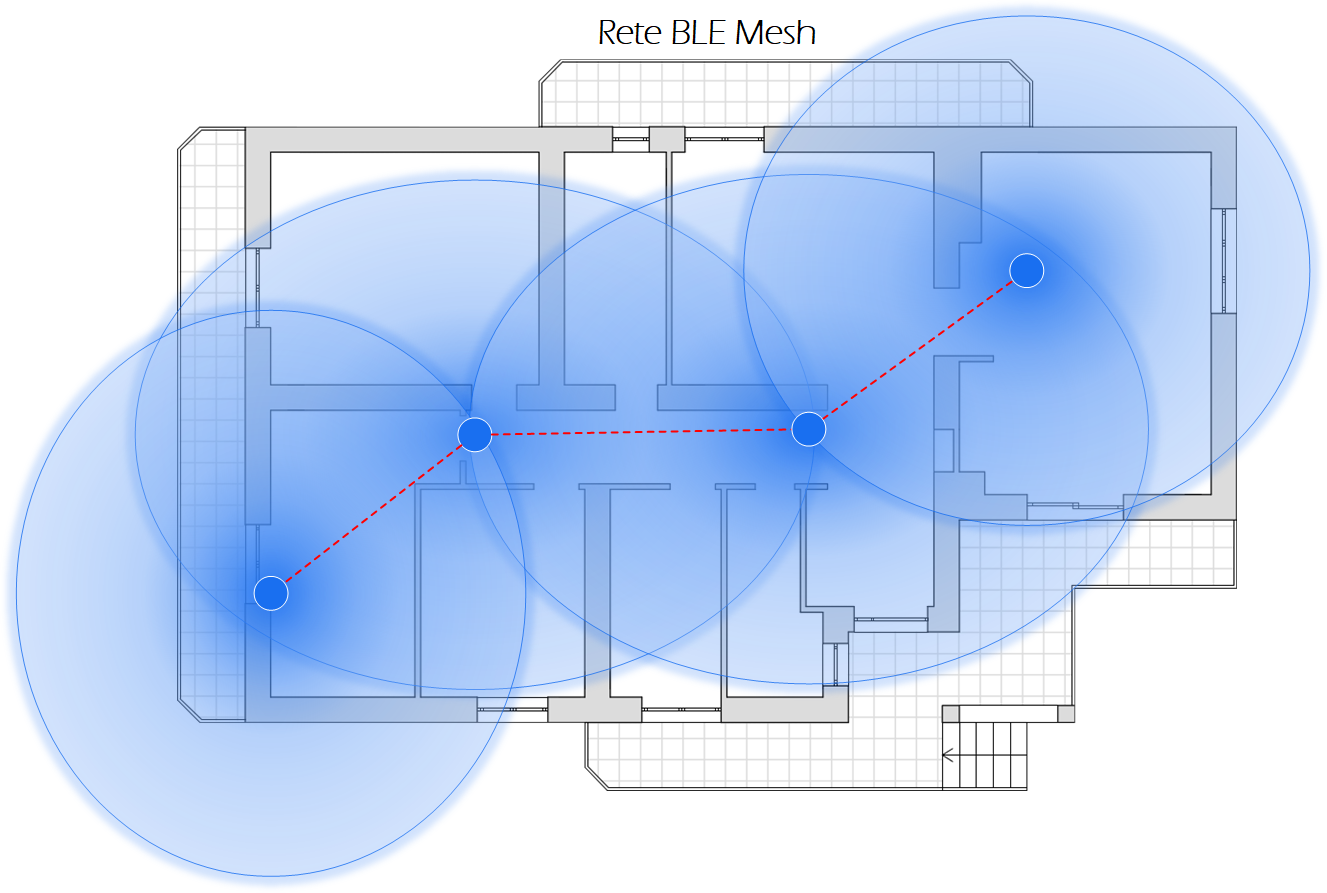
\includegraphics[width = 0.95\textwidth]{images/Rete_mesh_.png}
    \caption{Posizionamento dei nodi durante l'esecuzione di un test (\texttt{Configurazione 3})}
    \label{fig:rete_mesh}
\end{figure}

\noindent Al fine di studiare il comportamento della rete, utilizzando i due approcci descritti nei capitoli precedenti, sono stati definiti dei test in funzione alla distanza tra mittente e destinatario e all'aumentare del carico di lavoro.\\
Il variare della distanza ha portato alla definizione di tre configurazioni.
\begin{itemize}
    \item la configurazione \texttt{1} prevede l'impiego di due dispositivi soltanto (\texttt{Switch} e \texttt{Node-3}).
    \item la configurazione \texttt{2} prevede l'impiego di tre dispositivi. Il destinatario è stato posto ad una distanza maggiore e per garantire la comunicazione è stato necessario introdurre il nodo \texttt{relay-1}.
    \item la configurazione \texttt{3} prevede l'impiego di quattro dispositivi. Il destinatario è stato distanziato ulteriormente e quindi è stato necessario introdurre \texttt{relay-2} per garantire la comunicazione.
\end{itemize}

\noindent Il variare del carico di lavoro è stato gestito modificando la frequenza con cui i messaggi vengono immessi nella rete.
In tale circostanza sono stati presi in considerazione i seguenti periodi: \texttt{\textit{50ms}}, \texttt{\textit{100ms}}, \texttt{\textit{150ms}}, \texttt{\textit{200ms}}, \texttt{\textit{250ms}}, \texttt{\textit{500ms}} e \texttt{\textit{1000ms}}.\\
Il \textit{periodo} (\textit{T}), misurato in \textit{s}, è quella grandezza fisica che misura l'intervallo di tempo tra gli istanti iniziali di due eventi successivi.
La \textit{frequenza} (\textit{f}), misurata in \textit{Hz}, è quel fenomeno fisico che presenta un andamento costituito da eventi che si ripetono identici o quasi identici nel tempo e viene definita dal numero degli eventi che si ripetono in una data unità di tempo. Poiché la frequenza consente di esprimere meglio in concetto in merito al carico di lavoro della rete e può essere calcolata come l'inverso del periodo tramite la formula:
$$ f = \frac{1}{T} $$
si ottengono le seguenti valori (riportati nel medesimo ordine con cui sono stati espressi i periodi): \texttt{\textit{20 Hz}}, \texttt{\textit{10 Hz}}, \texttt{\textit{6.67 Hz}}, \texttt{\textit{5 Hz}}, \texttt{\textit{4 Hz}}, \texttt{\textit{2 Hz}} e \texttt{\textit{1 Hz}}.\\


\noindent Al fine di ottenere dei dati significativi per potere eseguire della analisi statistiche accurate, il test per ogni terna creata combinando \textit{configurazione}, \textit{frequenza} e \textit{approccio} hanno avuto una durata di \texttt{5} minuti e ripetuti \texttt{5} volte. Per garantire la medesima durata di ogni esperimento eseguito e allo stesso tempo avere carichi di lavoro ben distinti, il numero di messaggi inviati risulta essere inversamente proporzionane alla frequenza utilizzata.\\

\noindent L'insieme di tutti i test effettuati, ha comportato così una durata di circa 1050 minuti, ovvero circa \texttt{18} ore.

\section{Metriche}

\subsubsection{Latency}
La latenza o anche conosciuta come \textit{delay}, indica il tempo impiegato da una richiesta per passare dal mittente al ricevente e comprende anche il tempo impiegato dal destinatario per l'elaborazione del messaggio. La latenza in una rete è misurata in millisecondi e può essere misurata come il Round Trip Time (\texttt{RTT}) tra il client e il server. L'\texttt{RTT} è definito come la quantità di tempo impiegata da un pacchetto per giungere al destinatario e tornare indietro.\\
Tale valore è ottenuto mediante la differenza tra il tempo acquisito alla trasmissione del pacchetto (\texttt{start\_time}) e il tempo acquisito alla ricezione della relativa risposta (\texttt{final\_time}). Con tale calcolo otteniamo il \texttt{RTT}, mentre per determinare la latenza della rete, tale valore è stato ripartito per la fase di invio e la fase di ricezione, ovvero brutalmente diviso per due.
$$ latency = \frac{final\_time - start\_time}{2} $$

\subsubsection{Goodput}
Il Throughput misura la quantità di pacchetti scambiati (consegnati con successo) sulla rete, in un certo intervallo di tempo, al fine di determinare l'efficienza di tale rete. Il Goodput può essere definito come il Throughput a livello applicativo di una comunicazione. Ovvero, il numero di informazioni utili (misurate in bit) consegnate dalla rete ad una certa destinazione per unità di tempo.\\
La quantità di dati presi in considerazione comprende solo il Payload del messaggio, escludendo l'overhead richiesto dal protocollo per gestire l'intera trasmissione del pacchetto.\\
L'indice è calcolato dividendo la quantità di dati trasmessi con successo nell'unità di tempo. Non rientrano in questo conteggio i segmenti trasmessi con errore o duplicati. Il risultato viene rappresentato in Bps (Byte per second).
$$ goodput = \frac{pkt\_num \times pkt\_size}{time} $$

\noindent In cui \texttt{pkt\_num} indica il numero di pacchetti ricevuti correttamente durante l'intero test, \texttt{pkt\_size} indica la dimensione dell'informazione utile scambiata e \texttt{time} indica il tempo necessario alla ricezione di tutti i messaggi spediti.\\
Poiché con un payload superiore ad 11 byte il Lower Transport Layer prevede la segmentazione del pacchetto, la dimensione scelta risulta essere nettamente inferiore e legata al modello utilizzato (\texttt{Generic Level Set}). In tale circostanza l'informazione utile, ovvero lo \texttt{STATUS} dell'elemento è rappresentato impiegando 2 byte.

\subsubsection{Packet Delivery Ratio}
Il Packet Delivery Ratio (\texttt{PDR}) indica il tasso tra il numero di pacchetti ricevuti e il numero di pacchetti inviati attraverso la rete. 
$$ PDR = \frac{\sum packet\_received}{\sum packet\_sent} $$

\subsubsection{Intervalli di confidenza}
I risultati ottenuti utilizzando le metriche sopra descritte sono accompagnati da un intervallo di confidenza al fine di rendere precisa la stima del campione riportata.\\
L'intervallo di confidenza fornisce informazioni riguardo alla precisione dei valori ottenuti attraverso lo studio del campione. \\
Si è ricorso al calcolo dell'intervallo di confidenza poiché, la stima puntuale fornisce un valore singolo che varia a seconda del campione e difficilmente coincide con il valore vero della popolazione. Impiegando tale stima è possibile fornire un insieme di valori (un intervallo) che con una certa ``confidenza'' contiene il valore vero della popolazione.\\
In tale circostanza è stato calcolato un intervallo di confidenza del 95\%, in modo da affermare con una margine di certezza ragionevole (appunto 95\%) che quell'intervallo conterrà il valore vero dell'intera popolazione.\\

\noindent L'intervallo di confidenza al 95\% lo si ottiene mediante le seguente formule:
$$\bar{x} = \frac{\sum x}{n}$$
$$\sigma = \sqrt{\frac{\sum (x-\bar{x})^2}{n}}$$
$$\bar{x} \pm Z_{\alpha/2} \times \frac{\sigma}{\sqrt{n}}$$

\noindent in cui nella prima formula: $\bar{x}$ indica la media aritmetica della metrica in esame, $n$ indica la numerosità del campione e in tale circostanza coincide con il numero di run eseguiti per ogni tipologia di test (ovvero 5 run). La seconda formula consente di calcolare la deviazione standard (il grado di dispersione della distribuzione) ed indicata con la lettera greca sigma ($\sigma$). Le prime due formule sono impiegate nella terza formula per definire l'intervallo di confidenza, dove il simbolo $\pm$ permette il calcolo del limite inferiore e superiore dell'intervallo e $Z_{\alpha/2}$ indica il coefficiente di confidenza (poiché è stato scelto di calcolare l'intervallo di confidenza al 95\% tale valore coincide con $1.96$).

\section{Risultati}
In questa sezione vengono analizzati i risultati ottenuti in rispetto dei requisiti stabiliti e riguardanti le tre metriche precedentemente descritte.\\
I dati sono stati analizzati utilizzando degli script \texttt{python} in grado di acquisire le informazioni memorizzate nei file di log durante l'esecuzione dei test, ripulire i dati acquisiti, rimuovere il transiente iniziale (fase necessaria alla rete per giungere a pieno regime) in modo da analizzare il comportamento della rete quando risulta essere a pieno regime. Una volta ripuliti i dati secondo quanto descritto, sono stati elaborati utilizzando le suddette metriche ed infine generati i seguenti grafici per facilitare la comprensione del comportamento della rete mesh nelle varie situazioni.

\subsubsection{Risultati Bluetooth Mesh}
\noindent Con il seguente grafico relativo all'impiego della sola tecnologia Bluetooth Mesh si vuole mostrare come la rete, con l'aumentare del carico di lavoro e con l'incrementare del numero di nodi intermedi frapposti tra mittente e destinatario tende a diminuire di prestazione.\\

\noindent Un lieve calo prestazionale si intravede sin da subito ed è legato all'aumentare della distanza tra mittente e destinatario il che comporta ai pacchetti di dover attraversare dei nodi intermedi prima di giungere a destinazione. La relazione tra frequenza e prestazione della rete sono inversamente proporzionali, come era prevedibile. Vale a dire che all'aumentare della frequenza di trasmissione, la prestazione della rete tende a diminuire.

\begin{figure}[hbt!]
    \centering
    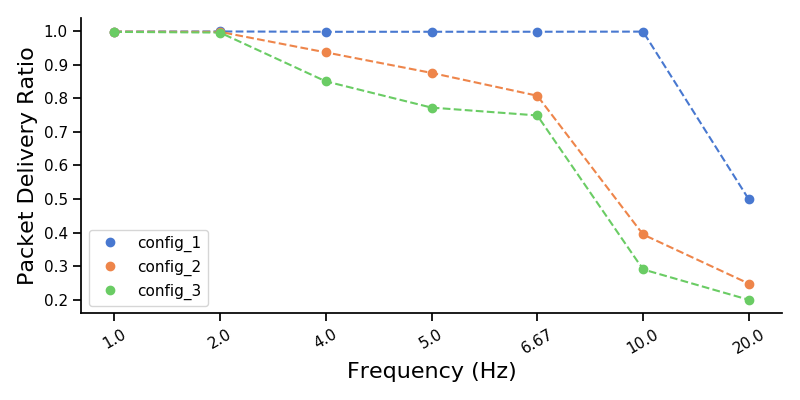
\includegraphics[width = 0.95\textwidth]{images/graphs/ble_pdr.png}
    \caption{Packed Delivery Ratio - Bluetooth Mesh}
    \label{graph:ble_pdr}
\end{figure}

\noindent Il punto in cui si evince così tanta differenza, per le \texttt{conf\_2} e \texttt{conf\_3}, riguarda l'impiego dei seguenti tassi trasmissivi: \texttt{150ms} (6.67 Hz) e \texttt{100ms} (10 Hz); mentre per la \texttt{conf\_1} tale situazione si verifica con l'impiego dei tassi trasmissivi: \texttt{100ms} (10 Hz) e \texttt{50ms} (20 Hz). \\
In quest'ultima circostanza il calo delle prestazioni è legato non solo al carico di lavoro che deve gestire la rete ma anche ai limiti imposti dalla tecnologia utilizzata. Per sopperire a tali perdite prestazionali si è fatto ricorso ad una tecnologia di supporto impiegata come descritto nei capitoli precedenti.\\

\noindent In merito alla \textit{latenza}, si può notare una variazione costante a partire dall'invio di messaggi ogni \texttt{150 ms}. La quale tende a raddoppiare nel momento in cui si passa da \texttt{conf\_2} a \texttt{conf\_3}. Analizzando più accuratamente il seguente grafico, si può notare una variazione impercettibile tra i \texttt{150 ms} e i \texttt{100 ms}, per poi aumentare nuovamente nel momento in cui si utilizza la frequenza più alta.

\begin{figure}[hbt!]
    \centering
    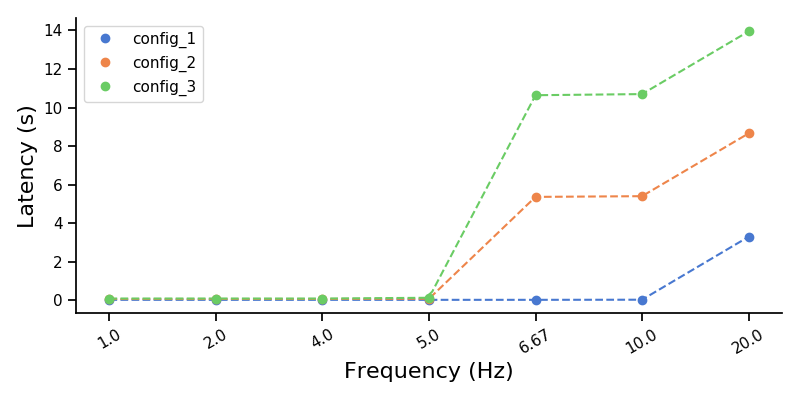
\includegraphics[width = 0.95\textwidth]{images/graphs/ble_latency.png}
    \caption{Latency - Bluetooth Mesh}
    \label{graph:ble_latency}
\end{figure}

\noindent I risultati in maniera dettagliata sono riportati in appendice, nella sezione \nameref{apex:outcomes_ble_mesh}. I valori sono rappresentati con tre cifre decimali al fine di facilitare la lettura. Per le tre metriche in esame sono riportati i valori \textit{medi} con accanto indicato il \textit{margine d'errore} al fine di affermare con una margine di certezza ragionevole l'intervallo che conterrà il valore vero dell'intera popolazione. Nei casi in cui il margine d'errore (\texttt{m\_e}) coincide con il valore $0.0$, vuol dire che esso è talmente piccolo (richiede più valori decimali) e viene approssimato a tale cifra.

\subsubsection{Risultati Approccio Misto}
Con l'introduzione della tecnologia di supporto si è ottenuto un maggiore livello prestazionale a cui però è soggetto un maggior consumo energetico oltre ad un leggero incremento della latenza, dovuta alla determinazione della perdita del pacchetto per poi inviarlo nuovamente. Utilizzando questa configurazione (con l'impiego dello stack Bluetooth Mesh e l'impiego dello stack Wi-Fi) si sono ottenuti i risultati descritti di seguito.\\

\noindent Come accade con la situazione descritta in precedenza, anche in tale circostanza si verifica un calo prestazionale della rete con l'aumentare dei nodi e delle frequenze trasmissive. La differenza di questo calo prestazionale sta proprio nei valori, poiché in tale circostanza il valore più basso (\texttt{conf\_3} - tasso d'invio di \texttt{50 ms}) riscontrato dall'esecuzione dei 5 run di simulazione è $0.924$, mentre con l'impiego della solo tecnologia Bluetooth Mesh, nella medesima situazione, il valore ottenuto è di gran lunga inferiore, ovvero $0.2$ $\pm$ $0.012$ (per maggiori dettagli visualizzare i grafici e le tabelle in appendice).

\begin{figure}[hbt!]
    \centering
    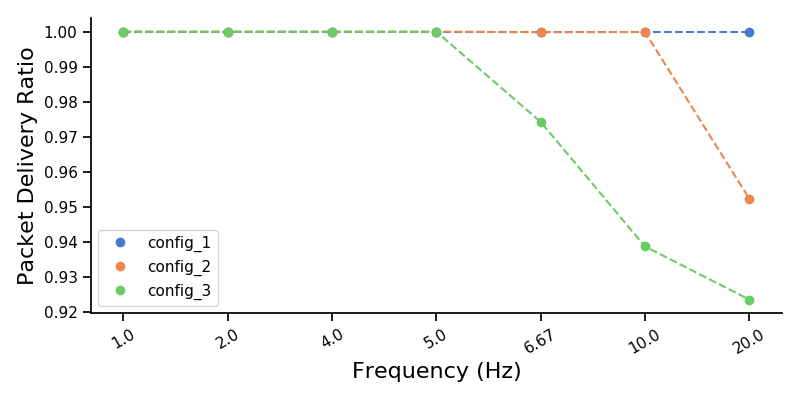
\includegraphics[width = 0.95\textwidth]{images/graphs/ble_wifi_pdr.png}
    \caption{Packed Delivery Ratio - Approccio Misto}
    \label{graph:ble_wifi_pdr}
\end{figure}

\noindent Come anticipato, l'introduzione dell'algoritmo misto introduce una certo ritardo al fine di determinare se un pacchetto effettivamente risulta essere perso oppure, a causa del carico di lavoro elevato con cui la rete sta operando, impiegherà più tempo del previsto per giungere a destinazione e successivamente tornare indietro.\\
L'algoritmo prevede un adeguamento piuttosto lento della soglia, proprio per far fronte ad una situazione del genere. La quale però, analizzando i risultati riportati nel grafico seguente e confrontati con il grafico dell'approccio Bluetooth Mesh (\nameref{graph:ble_latency}), si notano dei valori leggermente più alti. Un confronto immediato può essere eseguito analizzando il grafico relativo alla latenza in appendice, nella sezione \nameref{apex:grafici}.\\
Le curve, distinte in base alla configurazione, in entrambi i grafici presentano un andamento molto simile. Ovvero tendono a discostarsi dalla \texttt{configurazione 1} nel momento in cui si ha un tasso d'invio di \texttt{150 ms}.

\begin{figure}[hbt!]
    \centering
    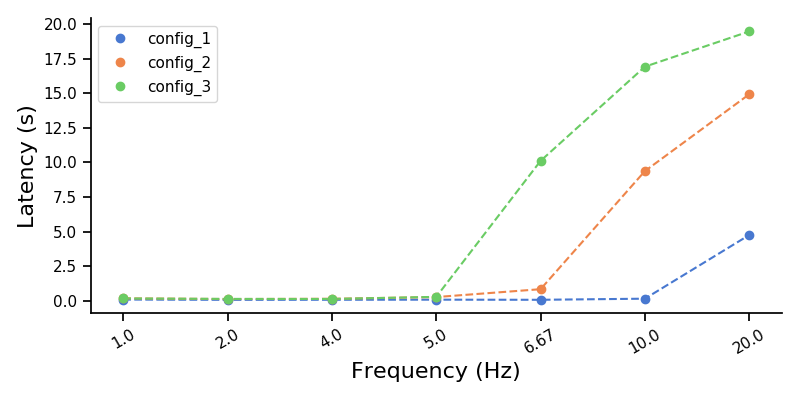
\includegraphics[width = 0.95\textwidth]{images/graphs/ble_wifi_latency.png}
    \caption{Latency - Approccio Misto}
    \label{graph:ble_wifi_latency}
\end{figure}

\noindent Con l'impiego dell'approccio misto, le prestazioni della rete risultano essere nettamente migliori e questo è percepibile analizzando il grafico relativo al goodput. A differenza della situazione verificata con l'altro approccio, qui si ha un andamento pressoché identico per tutte e tre le configurazioni. Garantendo di fatto l'efficacia dell'algoritmo implementato.

\begin{figure}[hbt!]
    \centering
    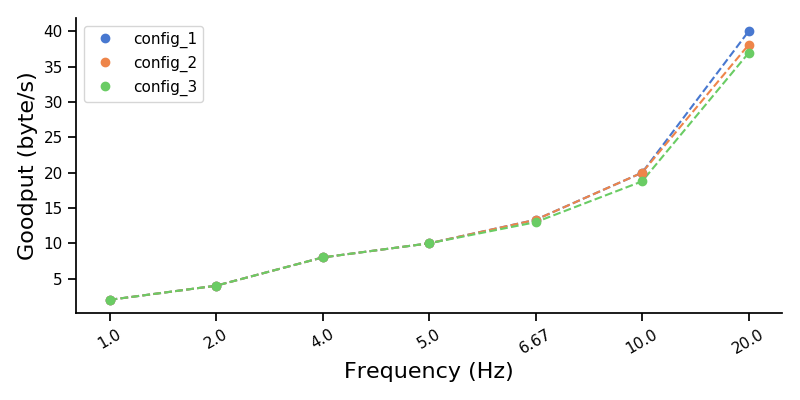
\includegraphics[width = 0.95\textwidth]{images/graphs/ble_wifi_goodput.png}
    \caption{Goodput - Approccio Misto}
    \label{graph:ble_wifi_goodput}
\end{figure}

\noindent Come indicato in precedenza, in appendice, nella sezione \textit{\nameref{apex:grafici}} è possibile osservare i grafici che riportano entrambe le situazioni, al fine di percepire in maniera molto più rapide le differenze e l'efficacia dell'algoritmo in termini prestazionali. I risultati in forma tabellare sono riportare in appendice, nella sezione \nameref{apex:outcomes_ble_wifi_mesh}. 
Solitamente i valori sono rappresentati con tre cifre decimali al fine di semplificare la lettura, ma nei casi in cui risultano essere talmente piccoli che non è possibile rappresentarli correttamente in tale modo, sono rappresentati in notazione scientifica utilizzando due decimali. Questa situazione si verifica con il margine d'errore (\texttt{m\_e}) poiché i valori ottenuti nelle 5 ripetizioni risultano molto simili tra loro. Nel caso in cui il valore è \texttt{0.0} vuol dire che non c'è stata nessuna perdita di pacchetto in tutte le ripetizioni e quindi si ottiene sempre il medesimo valore.\\

\noindent Analizzando più del dettaglio il file di log ottenuto tramite l'impiego dell'approccio misto è stato possibile individuare i pacchetti che sono con esito positivo distinguendoli in base alla tecnologia utilizzata. Nello specifico il seguente grafico mostra l'impiego delle due tecnologie attraverso una scala percentuale, calcolata sui pacchetti definiti come ricevuti con successo. Come ci si aspettava, aumentando la
frequenza di trasmissione il numero di pacchetti persi con la tecnologia Bluetooth risulta essere piuttosto elevato e di conseguenza c'è un maggior impiego della tecnologia WiFi, mentre con frequenza molto basse, tendenti ad 1 Hz, l'impiego della tecnologia WiFi risulta essere quasi assente. Come indicato in precedenza (nel descrivere i grafici inerenti le metriche calcolate), anche tale grafico ha il medesimo andamento dovuto all'incremento del numero di nodi intermedi per l'impiego di messaggi avallandosi della tecnologia Bluetooth. Ovvero, man mano che la distanza da mittente e destinatario e la frequenza d'invio tende ad aumentare, le prestazioni della rete tendono a diminuire e proprio in tale circostanze entra in gioco l'algoritmo dinamico implementato.

\begin{figure}[hbt!]
    \centering
    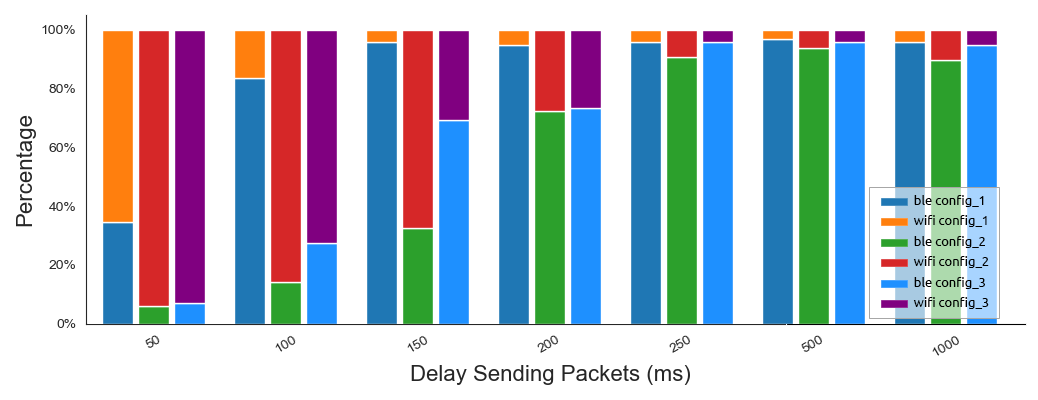
\includegraphics[width = 1\textwidth]{images/graphs/myplot_packets.png}
    \caption{Pacchetti ricevuti con successo - Approccio Misto}
    \label{graph:mix_packets_percentuage}
\end{figure}

\noindent Ulteriori grafici inerenti le tecnologie impiegate per la gestione della comunicazione tra mittente e destinatario sono presenti in appendice, nella sezione \textit{\nameref{apex:grafici_packets}}.



    \chapter{Conclusione}
\label{ch:conclusione}
Nel seguente elaborato di tesi è stata descritta la progettazione e la valutazione sperimentale di reti di monitoraggio mesh indoor basate su tecnologia Bluetooth Mesh.\\

\noindent Durante la prima fase è stato necessario uno studio preliminare degli aspetti tecnologici relativi alla situazione attuale in merito al mondo IoT, in modo da comprendere il progresso tecnologico che sta caratterizzando le reti di sensori e più nello specifico il nuovo standard rilasciato da Bluetooth SIG per consentire la comunicazione \textit{many-to-many} impiegando una radio Bluetooth. Tale standard opera al di sopra dello stack protocollare Bluetooth Low Energy, quindi, prima di procedere con la realizzazione di una rete mesh è stato necessario comprendere a pieno il protocollo sottostante.\\
Comprese le caratteristiche dei due standard forniti da Bluetooth SIG, si è passati alla comprensione del framework rilasciato da Espressif per configurare le proprie board e solo allora è stato possibile approfondire nel dettaglio l’impiego e l'utilizzo delle librerie messe a disposizione per realizzazione di una rete mesh di microcontrollori avvalendosi di dispositivi ESP32. La difficoltà maggiore ha riguardato l'utilizzo della libreria messa a disposizione da Espressif poiché non ancora in versione definitiva, quindi sempre in continua evoluzione. Evoluzione necessaria poiché il supporto a tale standard è piuttosto recente (secondo la documentazione, l'inizio di un progetto dedicato a Bluetooth Mesh è avvenuto a partire da gennaio 2019).\\
La scelta di focalizzare il lavoro sulle tecnologie Bluetooth e Wi-Fi ha riguardato principalmente la loro diffusione, ovvero oggigiorno sono presenti in qualsiasi tipologia di apparato di utilizzo quotidiano. Quindi utilizzando l'hardware comunemente a disposizione di chiunque è possibile creare un rete mesh, adoperando un software specifico sufficiente a garantire tale modalità di funzionamento.\\
Tra le due si è preferito il maggior impiego della tecnologia Bluetooth, poiché risulta essere meno dispendiosa energeticamente. In merito alla tecnologia Wi-Fi, purtroppo non è stato possibile utilizzarla in modalità Mesh, poiché i dispositivi in possesso, per questioni di memoria e di scarsa ottimizzazione delle librerie messe a disposizione dalla casa costruttrice, non sono in grado di eseguire i due stack contemporaneamente. Per fronteggiare tale situazione è stata utilizzata la tecnologia Bluetooth in modalità Mesh e quella Wi-Fi secondo il metodo convenzionale, ovvero con la presenza di un Access Point per garantire la comunicazione wireless tra i nodi della rete.\\
I risultati ottenuti dalle simulazioni eseguite utilizzando in combinazione lo standard Bluetooth Mesh e lo standard Wi-Fi hanno largamente soddisfatto quelle che erano le aspettative del seguente progetto di tesi.\\
In base ai risultati riscontrati dai test, la tecnologia Bluetooth Low Energy risulta essere efficiente dal punto di vista energetico ed in grado di garantire un'ottima copertura in un ambiente indoor piuttosto ampio andando ad utilizzare lo standard Bluetooth Mesh, oltre ad un basso costo delle componentistiche. L'unica nota dolente riguarda le sue prestazioni con un carico di lavoro piuttosto elevato, in cui si verificano elevate perdite di pacchetti. A tal proposito, utilizzando la tecnologia Wi-Fi è stato possibile alternare l'invio dei pacchetti tra le due tecnologie, garantendo così maggior affidabilità nella comunicazione.\\

% \noindent Il lavoro svolto si è dimostrato impegnativo in termini di impegno richiesto ma anche in termini di tempo, in quanto si è trattato di un progetto con tanti requisiti da soddisfare lato implementativo, il che hanno portato ad una lunga fase di validazione e valutazione. Tale lavoro e tale impegno sono stati ripagati con il soddisfacimento degli obiettivi preposti, ovvero andando ad eseguire su un medesimo nodo due stack protocollari differenti e alternare uno o l'altro in fase di comunicazione in modo da mantenere alte le prestazioni della rete, soprattutto nei casi in cui, utilizzando un unico stack, risulterebbe congestionata.


\section{Sviluppi Futuri}
Questo lavoro di tesi vuole essere un punto d'inizio per una serie di possibili sviluppi futuri che andrebbero sicuramente a migliorare molti aspetti, legati al comportamento del nodo in merito alle tecnologie di comunicazione impiegate, che per motivi di tempo non sono stati trattati.\\
Uno dei possibili sviluppi futuri può riguardare l'introduzione di intelligenza artificiale all'interno della rete, attraverso il paradigma di Machine Learning. Andando ad istruire il nodo attraverso tale tecnica, sarà in grado di acquisire conoscenza relativa all'ambiente circostanze, al carico di lavoro dell'intera rete e di come esso sia ripartito tra le due tecnologie, nonché le capacità di far fronte a tale situazione, le interferenze presenti in tale ambiente e le conseguenti perdite di pacchetti che si andranno a verificare.
Con tale base di conoscenza sarà in grado di effettuare delle scelte riguardanti la tecnologia da utilizzare per ogni singola comunicazione.
La scelta dovrà comunque tenere in considerazione i consumi energetici, in fase di trasmissione, della tecnologia utilizzata. 
Rispettando tale specifiche dovrà cercare allo stesso tempo di mantenere alte le prestazioni della rete, ovvero cercando di garantire sempre un Packet Delivery Ratio prossimo al valore 1.\\
Un altro progetto potrebbe prevedere il coinvolgimento di un'altra tipologia di standard da accostare a Bluetooth Mesh, con l'intendo di minimizzare i consumi energetici pur mantenendo alte le prestazioni della rete. Ad esempio, si potrebbe far ricorso ad una tecnologia appartenente alla categoria Wireless Personal Area Network, scegliendo tra ZigBee e 6LowPAN. Dopodiché eseguire le medesime sperimentazioni e confrontare i risultati acquisiti, al fine di poter decretare quale combinazione risulta essere meno dispendiosa e allo stesso tempo performante.
Un ulteriore progetto potrebbe inglobare il seguente lavoro ed eseguire ulteriori valutazioni prestazionali che, per questioni di tempo o di componenti non è stato possibile eseguire. Questo sviluppo potrebbe coinvolgere un misuratore di consumi energetici, in modo da misurare costantemente i consumi effettivi e applicare delle policy per regolamentarli. Un altro aspetto potrebbe riguardare la realizzazione di una rete più ampia, impiegando dei nodi aventi la feature di ``Friend'' attiva, in modo da inglobare anche i Low Power Node. Dopodiché ripetere le valutazioni prestazionali svolte o aggiungervene di nuove.
    
    \appendix

\chapter{Risultati Analisi}
\subsubsection{Tabelle Risultati - Bluetooth Mesh}
\label{apex:outcomes_ble_mesh}
\begin{table}[hbt!]
    \centering
    \begin{tabular}{ |rr|| c|c|c|c|c|c| } 
        \hline
%        \multicolumn{8}{|c|}{\textbf{Bluetooth Mesh} \texttt{configurazione 1}} \\
%        \hline \hline
        \multicolumn{2}{|c||}{\multirow{2}{*}{\textbf{Frequency}}} & \multicolumn{2}{|c|}{\textbf{Latency \scriptsize (s)}} & \multicolumn{2}{|c|}{\textbf{PDR}} & \multicolumn{2}{|c|}{\textbf{Goodput \scriptsize (bps)}} \\
        && \texttt{media} & \texttt{m\_e} & \texttt{media} & \texttt{m\_e} & \texttt{media} & \texttt{m\_e} \\

		\hline
		1 Hz & \scriptsize (1000 ms) & $ 0.025 $ & $ 0.001 $ & $ 0.998 $ & $ 0.002 $ & $ 1.997 $ & $ 0.004 $ \\
		\hline
		2 Hz & \scriptsize (500 ms) & $ 0.025 $ & $ 2.20 \times 10^{-4} $ & $ 0.999 $ & $ 0.001 $ & $ 3.995 $ & $ 0.004 $ \\
		\hline
		4 Hz & \scriptsize (250 ms) & $ 0.024 $ & $ 1.87 \times 10^{-4} $ & $ 0.998 $ & $ 0.001 $ & $ 7.982 $ & $ 0.005 $ \\
		\hline
		5 Hz & \scriptsize (200 ms) & $ 0.025 $ & $ 2.13 \times 10^{-4} $ & $ 0.998 $ & $ 0.001 $ & $ 9.978 $ & $ 0.007 $ \\
		\hline
		6.67 Hz & \scriptsize (150 ms) & $ 0.025 $ & $ 8.45 \times 10^{-5} $ & $ 0.998 $ & $ 0.001 $ & $ 13.305 $ & $ 0.016 $ \\
		\hline
		10 Hz & \scriptsize (100 ms) & $ 0.031 $ & $ 2.00 \times 10^{-4} $ & $ 0.998 $ & $ 0.001 $ & $ 19.965 $ & $ 0.012 $ \\
		\hline
		20 Hz & \scriptsize (50 ms) & $ 3.295 $ & $ 0.002 $ & $ 0.499 $ & $ 0.001 $ & $ 19.947 $ & $ 0.028 $ \\
		\hline
    \end{tabular}
    \caption{Risultati Analisi Bluetooth Mesh - \texttt{Configurazione 1}}
    \label{tab:table_ble_conf_1}
\end{table}

\begin{table}[hbt!]
    \centering
    \begin{tabular}{ |rr|| c|c|c|c|c|c| } 
        \hline
%        \multicolumn{8}{|c|}{\textbf{Bluetooth Mesh} \texttt{configurazione 2}} \\
%        \hline \hline
        \multicolumn{2}{|c||}{\multirow{2}{*}{\textbf{Frequency}}} & \multicolumn{2}{|c|}{\textbf{Latency \scriptsize (s)}} & \multicolumn{2}{|c|}{\textbf{PDR}} & \multicolumn{2}{|c|}{\textbf{Goodput \scriptsize (bps)}} \\
        && \texttt{media} & \texttt{m\_e} & \texttt{media} & \texttt{m\_e} & \texttt{media} & \texttt{m\_e} \\

		\hline
		1 Hz & \scriptsize (1000 ms) & $ 0.068 $ & $ 0.003 $ & $ 0.998 $ & $ 0.002 $ & $ 1.997 $ & $ 0.004 $ \\
		\hline
		2 Hz & \scriptsize (500 ms) & $ 0.069 $ & $ 0.001 $ & $ 0.997 $ & $ 0.001 $ & $ 3.99 $ & $ 0.003 $ \\
		\hline
		4 Hz & \scriptsize (250 ms) & $ 0.07 $ & $ 0.002 $ & $ 0.936 $ & $ 0.043 $ & $ 7.492 $ & $ 0.342 $ \\
		\hline
		5 Hz & \scriptsize (200 ms) & $ 0.082 $ & $ 0.001 $ & $ 0.875 $ & $ 0.032 $ & $ 8.753 $ & $ 0.322 $ \\
		\hline
		6.67 Hz & \scriptsize (150 ms) & $ 5.365 $ & $ 0.002 $ & $ 0.807 $ & $ 0.003 $ & $ 10.765 $ & $ 0.035 $ \\
		\hline
		10 Hz & \scriptsize (100 ms) & $ 5.402 $ & $ 0.003 $ & $ 0.394 $ & $ 0.01 $ & $ 7.883 $ & $ 0.203 $ \\
		\hline
		20 Hz & \scriptsize (50 ms) & $ 8.657 $ & $ 0.002 $ & $ 0.248 $ & $ 0.004 $ & $ 9.913 $ & $ 0.141 $ \\
		\hline
    \end{tabular}
    \caption{Risultati Analisi Bluetooth Mesh - \texttt{Configurazione 2}}
    \label{tab:table_ble_conf_2}
\end{table}

\begin{table}[hbt!]
    \centering
    \begin{tabular}{ |rr|| c|c|c|c|c|c| } 
        \hline
%        \multicolumn{8}{|c|}{\textbf{Bluetooth Mesh} \texttt{configurazione 3}} \\
%        \hline \hline
        \multicolumn{2}{|c||}{\multirow{2}{*}{\textbf{Frequency}}} & \multicolumn{2}{|c|}{\textbf{Latency \scriptsize (s)}} & \multicolumn{2}{|c|}{\textbf{PDR}} & \multicolumn{2}{|c|}{\textbf{Goodput \scriptsize (bps)}} \\
        && \texttt{media} & \texttt{m\_e} & \texttt{media} & \texttt{m\_e} & \texttt{media} & \texttt{m\_e} \\

		\hline
		1 Hz & \scriptsize (1000 ms) & $ 0.092 $ & $ 0.003 $ & $ 0.998 $ & $ 0.003 $ & $ 1.995 $ & $ 0.006 $ \\
		\hline
		2 Hz & \scriptsize (500 ms) & $ 0.093 $ & $ 4.15 \times 10^{-4} $ & $ 0.995 $ & $ 0.003 $ & $ 3.982 $ & $ 0.012 $ \\
		\hline
		4 Hz & \scriptsize (250 ms) & $ 0.092 $ & $ 0.007 $ & $ 0.85 $ & $ 0.139 $ & $ 6.802 $ & $ 1.114 $ \\
		\hline
		5 Hz & \scriptsize (200 ms) & $ 0.132 $ & $ 0.007 $ & $ 0.772 $ & $ 0.137 $ & $ 7.72 $ & $ 1.375 $ \\
		\hline
		6.67 Hz & \scriptsize (150 ms) & $ 10.64 $ & $ 0.015 $ & $ 0.749 $ & $ 0.014 $ & $ 9.982 $ & $ 0.187 $ \\
		\hline
		10 Hz & \scriptsize (100 ms) & $ 10.698 $ & $ 0.03 $ & $ 0.29 $ & $ 0.034 $ & $ 5.803 $ & $ 0.681 $ \\
		\hline
		20 Hz & \scriptsize (50 ms) & $ 13.949 $ & $ 0.009 $ & $ 0.2 $ & $ 0.012 $ & $ 7.983 $ & $ 0.462 $ \\
		\hline
    \end{tabular}
    \caption{Risultati Analisi Bluetooth Mesh - \texttt{Configurazione 3}}
    \label{tab:table_ble_conf_3}
\end{table}

\newpage
\subsubsection{Tabelle Risultati - Approccio Misto}
\label{apex:outcomes_ble_wifi_mesh}

\begin{table}[hbt!]
    \centering
    \begin{tabular}{ |rr|| c|c|c|c|c|c| } 
        \hline
%        \multicolumn{8}{|c|}{\textbf{Bluetooth Mesh - Wi-Fi} \texttt{configurazione 1}} \\
%        \hline \hline
        \multicolumn{2}{|c||}{\multirow{2}{*}{\textbf{Frequency}}} & \multicolumn{2}{|c|}{\textbf{Latency \scriptsize (s)}} & \multicolumn{2}{|c|}{\textbf{PDR}} & \multicolumn{2}{|c|}{\textbf{Goodput \scriptsize (bps)}} \\
        && \texttt{media} & \texttt{m\_e} & \texttt{media} & \texttt{m\_e} & \texttt{media} & \texttt{m\_e} \\

		\hline
		1 Hz & \scriptsize (1000 ms) & $ 0.076 $ & $ 0.018 $ & $ 1.0 $ & $ 0.0 $ & $ 2.0 $ & $ 0.0 $ \\
		\hline
		2 Hz & \scriptsize (500 ms) & $ 0.055 $ & $ 0.004 $ & $ 1.0 $ & $ 0.0 $ & $ 4.0 $ & $ 0.0 $ \\
		\hline
		4 Hz & \scriptsize (250 ms) & $ 0.059 $ & $ 0.007 $ & $ 1.0 $ & $ 0.0 $ & $ 8.0 $ & $ 0.0 $ \\
		\hline
		5 Hz & \scriptsize (200 ms) & $ 0.067 $ & $ 0.01 $ & $ 1.0 $ & $ 0.0 $ & $ 10.0 $ & $ 0.0 $ \\
		\hline
		6.67 Hz & \scriptsize (150 ms) & $ 0.058 $ & $ 0.005 $ & $ 1.0 $ & $ 0.0 $ & $ 13.333 $ & $ 0.0 $ \\
		\hline
		10 Hz & \scriptsize (100 ms) & $ 0.138 $ & $ 0.005 $ & $ 1.0 $ & $ 0.0 $ & $ 20.0 $ & $ 0.0 $ \\
		\hline
		20 Hz & \scriptsize (50 ms) & $ 4.747 $ & $ 0.026 $ & $ 1.0 $ & $ 0.0 $ & $ 40.0 $ & $ 0.0 $ \\
		\hline
    \end{tabular}
    \caption{Risultati Analisi Approccio Misto - \texttt{Configurazione 1}}
    \label{tab:table_ble_wifi_conf_1}
\end{table}

\begin{table}[hbt!]
    \centering
    \begin{tabular}{ |rr|| c|c|c|c|c|c| } 
        \hline
%        \multicolumn{8}{|c|}{\textbf{Bluetooth Mesh - Wi-Fi} \texttt{configurazione 2}} \\
%        \hline \hline
        \multicolumn{2}{|c||}{\multirow{2}{*}{\textbf{Frequency}}} & \multicolumn{2}{|c|}{\textbf{Latency \scriptsize (s)}} & \multicolumn{2}{|c|}{\textbf{PDR}} & \multicolumn{2}{|c|}{\textbf{Goodput \scriptsize (bps)}} \\
        && \texttt{media} & \texttt{m\_e} & \texttt{media} & \texttt{m\_e} & \texttt{media} & \texttt{m\_e} \\

		\hline
 		1 Hz & \scriptsize (1000 ms) & $ 0.163 $ & $ 0.048 $ & $ 1.0 $ & $ 0.0 $ & $ 2.0 $ & $ 0.0 $ \\
		\hline
		2 Hz & \scriptsize (500 ms) & $ 0.112 $ & $ 0.017 $ & $ 1.0 $ & $ 0.0 $ & $ 4.0 $ & $ 0.0 $ \\
		\hline
		4 Hz & \scriptsize (250 ms) & $ 0.131 $ & $ 0.011 $ & $ 1.0 $ & $ 0.0 $ & $ 8.0 $ & $ 0.0 $ \\
		\hline
		5 Hz & \scriptsize (200 ms) & $ 0.256 $ & $ 0.079 $ & $ 1.0 $ & $ 0.0 $ & $ 10.0 $ & $ 0.0 $ \\
		\hline
		6.67 Hz & \scriptsize (150 ms) & $ 0.826 $ & $ 0.225 $ & $ 1.0 $ & $ 2.19 \times 10^{-4} $ & $ 13.332 $ & $ 0.003 $ \\
		\hline
		10 Hz & \scriptsize (100 ms) & $ 9.375 $ & $ 0.201 $ & $ 1.0 $ & $ 1.46 \times 10^{-4} $ & $ 19.998 $ & $ 0.003 $ \\
		\hline
		20 Hz & \scriptsize (50 ms) & $ 14.937 $ & $ 0.028 $ & $ 0.952 $ & $ 0.05 $ & $ 38.093 $ & $ 1.987 $ \\
		\hline
    \end{tabular}
    \caption{Risultati Analisi Approccio Misto - \texttt{Configurazione 2}}
    \label{tab:table_ble_wifi_conf_2}
\end{table}

\begin{table}[hbt!]
    \centering
    \begin{tabular}{ |rr|| c|c|c|c|c|c| } 
        \hline
%        \multicolumn{8}{|c|}{\textbf{Bluetooth Mesh - Wi-Fi} \texttt{configurazione 3}} \\
%        \hline \hline
        \multicolumn{2}{|c||}{\multirow{2}{*}{\textbf{Frequency}}} & \multicolumn{2}{|c|}{\textbf{Latency \scriptsize (s)}} & \multicolumn{2}{|c|}{\textbf{PDR}} & \multicolumn{2}{|c|}{\textbf{Goodput \scriptsize (bps)}} \\
        && \texttt{media} & \texttt{m\_e} & \texttt{media} & \texttt{m\_e} & \texttt{media} & \texttt{m\_e} \\

		\hline
		1 Hz & \scriptsize (1000 ms) & $ 0.154 $ & $ 0.033 $ & $ 1.0 $ & $ 0.0 $ & $ 2.0 $ & $ 0.0 $ \\
		\hline
		2 Hz & \scriptsize (500 ms) & $ 0.122 $ & $ 0.008 $ & $ 1.0 $ & $ 0.0 $ & $ 4.0 $ & $ 0.0 $ \\
		\hline
		4 Hz & \scriptsize (250 ms) & $ 0.118 $ & $ 0.013 $ & $ 1.0 $ & $ 0.0 $ & $ 8.0 $ & $ 0.0 $ \\
		\hline
		5 Hz & \scriptsize (200 ms) & $ 0.27 $ & $ 0.098 $ & $ 1.0 $ & $ 0.0 $ & $ 10.0 $ & $ 0.0 $ \\
		\hline
		6.67 Hz & \scriptsize (150 ms) & $ 10.115 $ & $ 1.09 $ & $ 0.974 $ & $ 0.003 $ & $ 12.99 $ & $ 0.042 $ \\
		\hline
		10 Hz & \scriptsize (100 ms) & $ 16.933 $ & $ 0.205 $ & $ 0.939 $ & $ 2.73 \times 10^{-4} $ & $ 18.773 $ & $ 0.005 $ \\
		\hline
		20 Hz & \scriptsize (50 ms) & $ 19.485 $ & $ 0.013 $ & $ 0.924 $ & $ 4.38 \times 10^{-4} $ & $ 36.94 $ & $ 0.018 $ \\
		\hline
    \end{tabular}
    \caption{Risultati Analisi Approccio Misto - \texttt{Configurazione 3}}
    \label{tab:table_ble_wifi_conf_3}
\end{table}

\subsubsection{Grafici Risultati Analisi}
\label{apex:grafici}

\begin{figure}[hbt!]
    \centering
    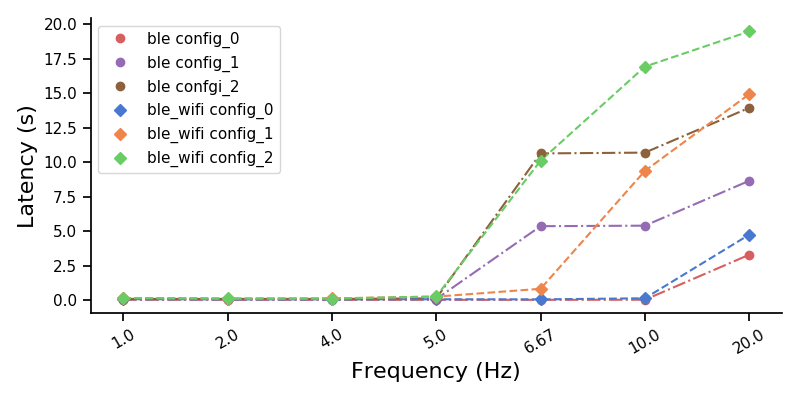
\includegraphics[width = 1\textwidth]{images/graphs/mixed_latency.png}
    \caption{\texttt{Latency} - Confronto Bluetooth Mesh e Approccio Misto}
    \label{graph:mixed_latency}
\end{figure}

\begin{figure}[hbt!]
    \centering
    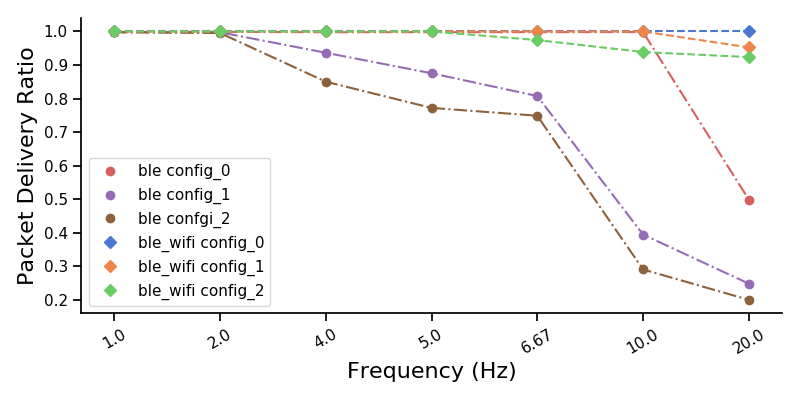
\includegraphics[width = 1\textwidth]{images/graphs/mixed_pdr.png}
    \caption{\texttt{Packet Delivery Ratio} - Confronto Bluetooth Mesh e Approccio Misto}
    \label{graph:mixed_pdr}
\end{figure}

\begin{figure}[hbt!]
    \centering
    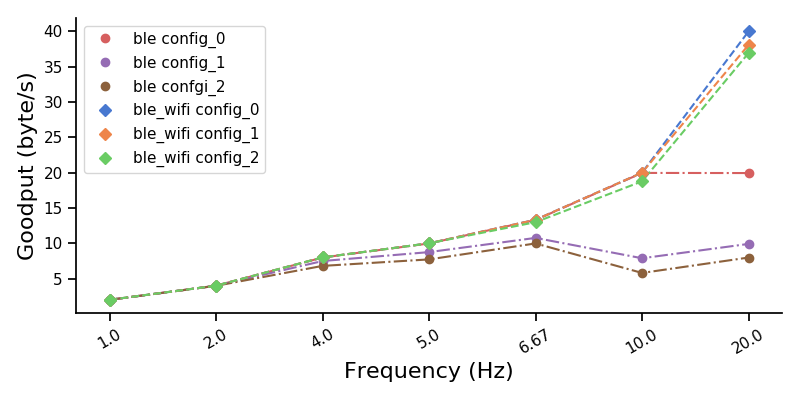
\includegraphics[width = 1\textwidth]{images/graphs/mixed_goodput.png}
    \caption{\texttt{Goodput} - Confronto Bluetooth Mesh e Approccio Misto}
    \label{graph:mixed_goodput}
\end{figure}

\clearpage
\subsubsection{Tabella e Grafici gestione pacchetti - Approccio Misto}
\label{apex:grafici_packets}

\begin{table}[hbt!]
    \centering
    \begin{tabular}{ |rr|| c|c|| c|c|| c|c| } 
        \hline
%        \multicolumn{8}{|c|}{\textbf{Bluetooth Mesh - Wi-Fi} \texttt{configurazione 3}} \\
%        \hline \hline

        \multicolumn{2}{|c||}{\multirow{2}{*}{\textbf{Frequency}}} & \multicolumn{2}{|c||}{\textbf{Config. 1}} & \multicolumn{2}{|c||}{\textbf{Config. 2}} & \multicolumn{2}{|c|}{\textbf{Config. 3}} \\
        && \texttt{ BLE } & \texttt{Wi-Fi} & \texttt{ BLE } & \texttt{Wi-Fi}& \texttt{ BLE } & \texttt{Wi-Fi} \\
		\hline
		1 Hz & \scriptsize (1000 ms) & $ 95 \% $ & $ 5 \% $ & $ 94 \% $ & $ 6 \% $ & $ 89 \% $ & $ 11 \% $  \\
		\hline
		2 Hz & \scriptsize (500 ms) & $ 96 \% $ & $ 4 \% $ & $ 95 \% $ & $ 5 \% $ & $ 93 \% $ & $ 7 \% $  \\
		\hline
		4 Hz & \scriptsize (250 ms) & $ 95 \% $ & $ 5 \% $ & $ 95 \% $ & $ 5 \% $ & $ 90 \% $ & $ 10 \% $  \\
		\hline
		5 Hz & \scriptsize (200 ms) & $ 94 \% $ & $ 6 \% $ & $ 73 \% $ & $ 27 \% $ & $ 72 \% $ & $ 28 \% $  \\
		\hline
		6.67 Hz & \scriptsize (150 ms) & $ 95 \% $ & $ 5 \% $ & $ 69 \% $ & $ 31 \% $ & $ 33 \% $ & $ 67 \% $ \\
		\hline
		10 Hz & \scriptsize (100 ms) & $ 83 \% $ & $ 17 \% $ & $ 28 \% $ & $ 72 \% $ & $ 15 \% $ & $ 85 \% $  \\
		\hline
		20 Hz & \scriptsize (50 ms) & $ 35 \% $ & $ 65 \% $ & $ 8 \% $ & $ 92 \% $ & $ 7 \% $ & $ 93 \% $  \\
		\hline
    \end{tabular}
    \caption{Percentuali impiego tecnologie durante la fase di test}
    \label{tab:table_perc_ble_wifi}
\end{table}

\begin{figure}[hbt!]
    \centering
    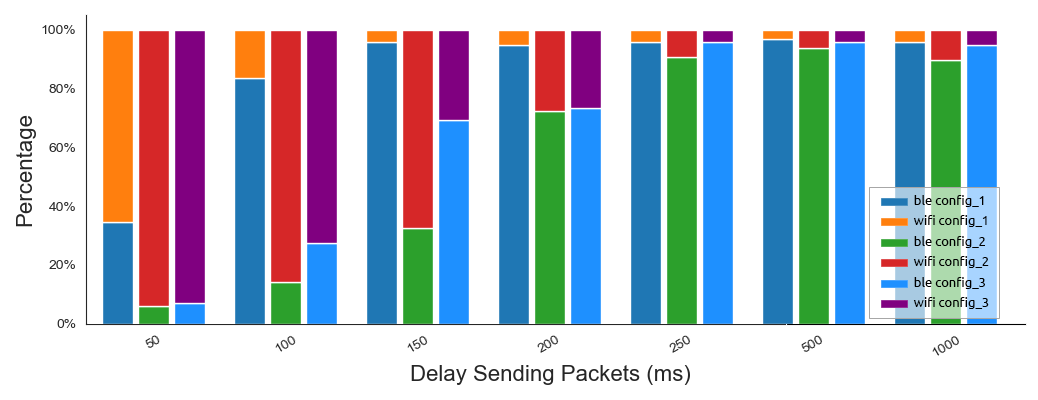
\includegraphics[width = 1\textwidth]{images/graphs/myplot_packets.png}
    \caption{Gestione pacchetti Approccio Misto - Confronto}
    \label{graph:mix_packets_percentuage}
\end{figure}

%\begin{figure}[hbt!]
%    \centering
%    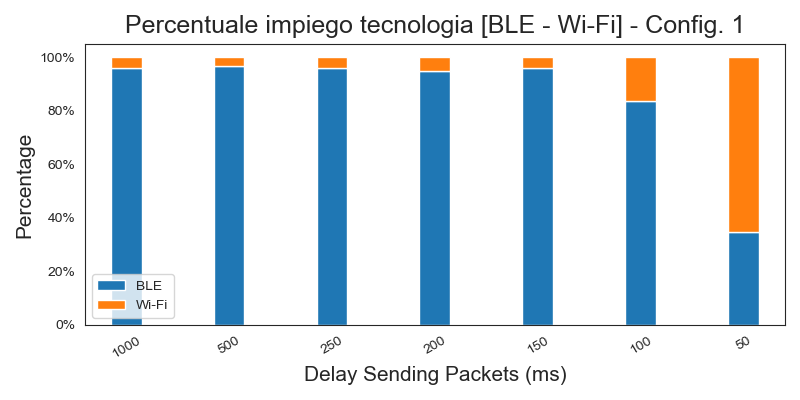
\includegraphics[width = 1\textwidth]{images/graphs/myplot_config_1_title.png}
%    \caption{Tecnologia gestione pacchetti - Approccio Misto - Configurazione 1}
%    \label{graph:mixed_conf_1}
%\end{figure}
%\begin{figure}[hbt!]
%    \centering
%    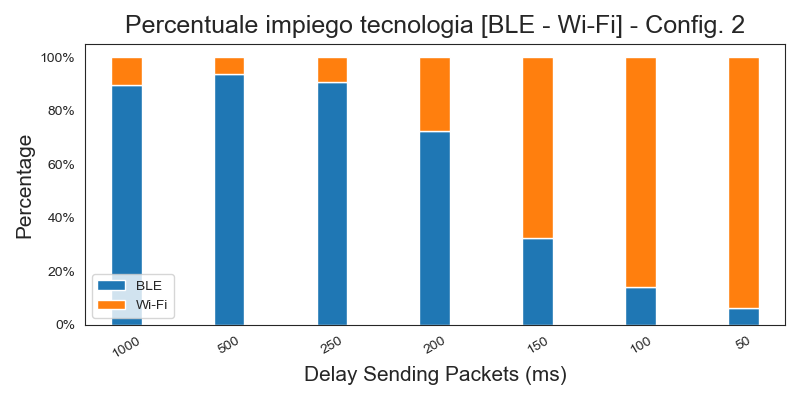
\includegraphics[width = 1\textwidth]{images/graphs/myplot_config_2_title.png}
%    \caption{Tecnologia gestione pacchetti - Approccio Misto - Configurazione 2}
%    \label{graph:mixed_conf_2}
%\end{figure}
%\begin{figure}[hbt!]
%    \centering
%    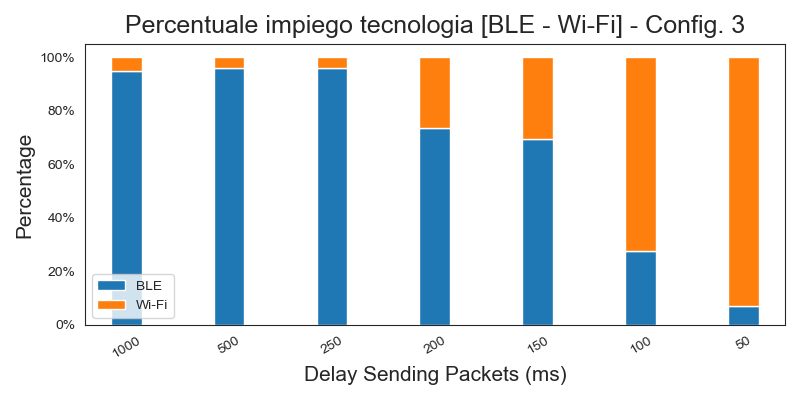
\includegraphics[width = 1\textwidth]{images/graphs/myplot_config_3_title.png}
%    \caption{Tecnologia gestione pacchetti - Approccio Misto - Configurazione 3}
%    \label{graph:mixed_conf_3}
%\end{figure}
    
    % === Bibliografia ====================================
    \cleardoublepage
    \addcontentsline{toc}{chapter}{Bibliografia}
    \printbibheading
    \printbibliography[type=article,heading=subbibliography,title={Articoli}]
    \printbibliography[type=book,heading=subbibliography,title={Libri}]
    \printbibliography[keyword={online},heading=subbibliography,title={Online}]

    % === Ringraziamenti ====================================
    \chapter*{Ringraziamenti}
\thispagestyle{empty}
\pagestyle{empty}
Eccomi giunto alla fine di questa tesi e di questi splendidi anni universitari, nei quali credo di essere maturato come professionista in quella mia grande passione che è l'Informatica, ma anche e soprattutto come persona. Sono tante le conoscenze che ho fatto durante questo percorso, le amicizie che ho coltivato, i rapporti che ho stretto. Vorrei dedicare queste ultime pagine per ringraziare tutte le persone che hanno sempre creduto in me e che mi hanno sempre sostenuto sia nei momenti di difficoltà sia in quelli felici e spensierati. Vorrei che questi ringraziamenti siano un punto d'arrivo (per la carriera universitaria), ma anche un punto d'inizio, perché credo che non si finisca mai di crescere e spero di poter raggiungere nuovi traguardi importanti nella mia vita con tutti voi ancora al mio fianco.\\

\noindent In primis vorrei ringraziare il mio Relatore, Prof. Marco Di Felice, non solo per la fiducia accordatami accettando il ruolo di Relatore e affidandomi un progetto così innovativo, ma soprattutto per avermi spronato nel fare sempre di più e non accontentarsi mai dei traguardi raggiunti, ma spingersi sempre oltre, per poter raggiungerne di nuovi.
Inoltre lo ringrazio per la professionalità, la chiarezza e la pazienza con cui mi ha seguito durante la stesura del mio elaborato, ma anche per tutto ciò che mi ha insegnato durante il suo corso, suscitando in me un forte interesse nell'ambito dell'Internet of Things.\\ 
Il mio Correlatore, il Dottor Angelo Trotta per la disponibilità e la pazienza dimostrata ogni qual volta mi recavo da lui per avere maggiori delucidazioni sull'argomento, per i preziosi consigli divulgati e soprattutto per avermi trasmesso una forte passione su questa tematica.\\

\noindent Un doveroso ringraziamento va ovviamente alla mia famiglia, senza la quale non avrei mai neppur cominciato questa carriera. Mi è sempre stata accanto e non ha fatto mai mancare il suo sostegno e il suo aiuto durante tutti questi anni. Grazie perché senza di voi non sarei mai arrivato fino in fondo a questo difficile, lungo e tortuoso cammino. Senza di voi non sarei mai diventato quello che sono e non avrei potuto coronare i miei molteplici sogni.\\
Ai miei genitori, che sono il mio punto di riferimento e che mi hanno sostenuto sia economicamente che emotivamente. Questa tesi la dedico a voi che siete la mia famiglia, il mio più grande sostegno e la mia guida.\\

\noindent Vorrei ringraziare Mario, un amico, un compagno di mille avventure, un ragazzo con cui ho condiviso attività di qualsiasi genere partendo dallo sport fino al sociale. So che per qualsiasi cosa potrò contare sempre su di te.\\

\noindent Un ringraziamento speciale a Simone e Aldo, che spinti dalle stesse passioni abbiamo condiviso tantissime esperienze assieme fino a diventare anche coinquilini, e che coinquilini. A seguito delle differenti scelte e delle carriere intraprese, ci siamo dovuti allontanare, ma la nostra amicizia non ha paura di una tale distanza, anche perché, le amicizie, quelle vere sono in grado di resistere al tempo, alle distanze e al silenzio. So che possiamo sempre contare gli uni sugli altri. \\

\noindent Vorrei ringraziare anche Angelo, che è stato più che un coinquilino. Nel corso di questi anni si è rivelato un vero e sopratutto simpaticissimo amico, sempre pronto ad ascoltarti e ad aiutarti. Il legame che si è creato del corso del tempo resterà forte e duraturo nonostante i numerosi chilometri che ci separano. Anche se ora, a seguito delle tue scelte, risultano essere molto di meno.\\

\noindent Un altro ringraziamento speciale voglio dedicarlo a Cristina, che nonostante la lontananza è sempre presente, pronta a spronarmi nelle mie scelte e a dispensare preziosi consigli. Vorrei ringraziare anche Annamaria per le innumerevoli serate trascorse assieme, talvolta quasi a sfiorar l'alba, nonostante il mattino seguente dovevi svegliarti presto per andare al lavoro. Inoltre, voglio ringraziane tutti gli amici di Casacalenda, i quali hanno tutti avuto un peso nel conseguimento di questo risultato e che mi accolgono sempre a braccia aperte ad ogni mio rientro. Nominarvi tutti sarebbe impossibile.\\

\noindent Vorrei ringraziare Massimiliano, compagno di mille avventure universitarie. Sei stato il primo ragazzo conosciuto in triennale e da allora siamo stati sempre uno di fianco all'altro, uniti dalle stesse passioni, nell'affrontare le scelte relative alla specialistica e soprattutto gli innumerevoli progetti accademici. \\
Un ringraziamento speciale va ad Antonio, Francesco e Federico con i quali oltre a condividere questo fantastico percorso, è nata una splendida amicizia, che va al di fuori dell'ambito accademico. Grazie a loro e a Massi è stato possibile trascorrere fantastiche giornate, ma molto spesso anche pranzi, cene, etc. in giro per la bella Bologna.  \\

\noindent \texttt{Last but not least}, vorrei ringraziare due persone che ho conosciuto molto recentemente, ma si sono dimostrate sin da subito ottime compagne di viaggio. Seppur breve, per causa di forza maggiore, ma ha permesso, di esaltare, sin da subito, la vostra disponibilità e generosità sotto tutti i punti di vista. Vi ringrazio per aver reso meno pesanti, ma soprattutto molto più allegre quelle giornate in cui tutto era piuttosto grigio, a partire dalle ansie vissute e dallo studio, doveroso per superare il tanto temuto last exam, che in fondo è stata proprio la motivazione che ha sancito la nascita di questa stupenda amicizia. Grazie anche per le stupende giornate, seppur poche, passate assieme in quel di Bolo. Grazie Benedetta e grazie Chiara per essere state sempre al mio fianco, anche in un periodo difficile come questo e per aver sopportato e cercato di affievolire le mie ansie. 
Un immenso grazie a Benedetta per esserti dimostrata sin da subito una persona fantastica, con cui confidarsi e poter trascorrere stupende conversazioni, ma soprattutto voglio esprimere un caloroso ringraziamento per il prezioso tempo che hai dedicato nello scovare i refusi da me commessi. 
Grazie Chiara per avere reso non solo le giornate molto più allegre ma anche per aver reso il rientro verso i nostri alloggi molto più divertenti e meno duri, poiché guidati da splendide conversazioni.
Purtroppo il tempo trascorso assieme è stato davvero poco a causa di questo \texttt{COVID-19}, ma avremo modo e tempo per rifarci a conclusione di tutto ciò. Nel ringraziarvi, vi auguro anche un forte in bocca al lupo per il superamento di questo ostico ostacolo che, in fondo, ha sancito la nascita di questa brillante amicizia.\\

\noindent Ringrazio tutte le persone che non ho nominato esplicitamente in questa pagina, ma che hanno avuto un ruolo importante nella mia vita, perché i ricordi di tutti voi sono impressi in maniera indelebile nel mio cuore.
\end{document}